\documentclass[11pt, a4paper]{article}
\usepackage[utf8]{inputenc}
\usepackage{graphicx}
\usepackage{float}
\usepackage{titling}
\usepackage{titlesec}
\usepackage{amsmath}
\usepackage[font=small,labelfont=bf]{caption}
\usepackage[margin=1in]{geometry}
\usepackage[table,xcdraw]{xcolor}
\usepackage{gensymb}
\usepackage{lineno}
\usepackage{setspace}
\doublespacing
%\setlength{\droptitle}{-10em}
\vspace{1.5 \baselineskip}


\newcommand\wordcount{\documentclass[11pt, a4paper]{article}
\usepackage[utf8]{inputenc}
\usepackage{graphicx}
\usepackage{float}
\usepackage{titling}
\usepackage{titlesec}
\usepackage{amsmath}
\usepackage[font=small,labelfont=bf]{caption}
\usepackage[margin=1in]{geometry}
\usepackage[table,xcdraw]{xcolor}
\usepackage{gensymb}
\usepackage{lineno}
\usepackage{setspace}
\doublespacing
%\setlength{\droptitle}{-10em}
\vspace{1.5 \baselineskip}


\newcommand\wordcount{\documentclass[11pt, a4paper]{article}
\usepackage[utf8]{inputenc}
\usepackage{graphicx}
\usepackage{float}
\usepackage{titling}
\usepackage{titlesec}
\usepackage{amsmath}
\usepackage[font=small,labelfont=bf]{caption}
\usepackage[margin=1in]{geometry}
\usepackage[table,xcdraw]{xcolor}
\usepackage{gensymb}
\usepackage{lineno}
\usepackage{setspace}
\doublespacing
%\setlength{\droptitle}{-10em}
\vspace{1.5 \baselineskip}


\newcommand\wordcount{\documentclass[11pt, a4paper]{article}
\usepackage[utf8]{inputenc}
\usepackage{graphicx}
\usepackage{float}
\usepackage{titling}
\usepackage{titlesec}
\usepackage{amsmath}
\usepackage[font=small,labelfont=bf]{caption}
\usepackage[margin=1in]{geometry}
\usepackage[table,xcdraw]{xcolor}
\usepackage{gensymb}
\usepackage{lineno}
\usepackage{setspace}
\doublespacing
%\setlength{\droptitle}{-10em}
\vspace{1.5 \baselineskip}


\newcommand\wordcount{\input{write_up.sum}}

\newcommand{\beginsupplement}{%
        \setcounter{table}{0}
        \renewcommand{\thetable}{S\arabic{table}}%
        \setcounter{figure}{0}
        \renewcommand{\thefigure}{S\arabic{figure}}%
}


\setcounter{secnumdepth}{0}
\begin{document}

    \begin{titlepage}
	\centering
	
\includegraphics[width=0.5\textwidth]{../data/imperial.png}\par\vspace{1cm}
	\vspace{2cm}
	{\scshape\Large\bfseries Recommendations for Fitting Microbial Growth Models\par}
	\vspace{2cm}
	{\Large Sam Turner\par}
	\vspace{0.5cm}
	{\Large March 2020 \par}
	\vspace{0.5cm}
	{\Large\itshape Computational Method in Ecology and Evolution MSc\par}
	\vspace{0.5cm}
	 \wordcount words 
	\vfill

	\vfill
    
    \newpage
    \end{titlepage}
    

    \begin{abstract}
   Modelling of microbial growth is vital for developing food preservation measures to decrease food waste. By fitting a range of mechanistic and phenomenological models to a large dataset of 305 growth curves, I demonstrate that temperature has a major impact on microbial population dynamics. I also examine how methodological choices can influence the results of model fitting studies, including demonstrating that the choice of model can systematically bias parameter estimates to the extent that they become incomparable for meta-analysis. Improvements in the resolution of parameter estimates when models are fit in logarithmic space relative to linear space model fitting are also reported. These findings result in recommendations for microbial modelling methodology, particularly when data are aggregated across sources.
\end{abstract}
\tableofcontents
\begin{linenumbers}
    \section{Introduction}
    
    There is great interest in modelling the growth of microbial populations, in order to understand their response to external variables \cite{zwitmodelling}. This allows prediction of shelf lifes and optimisation of preservation methods. In this project, I address four questions:    

\begin{enumerate}
  \item Which models best describe microbial population growth, and how does this vary with temperature?
  \item How does temperature affect microbial growth?
  \item How does choice of model affects parameter estimates?
  \item Does the choice to fit models in linear or logarithmic space affect results?
  \end{enumerate}


I addressed these by fitting mechanistic and phenomenological models to a dataset of 305 digitised growth curves. Each mechanistic models describes the growth curve with a mathematical relationship representing a hypothesis about the dynamics of microbial growth \cite{Buchanan}, so is parameterised with meaningful biological quantities. In contrast, the phenomenological models are simply convenient mathematical functions used to describe patterns in the data, and are used as a neutral comparison for the mechanistic models. By comparing the fit of the mechanistic models to each other, and to the phenomenological models, support for the underlying biological hypothesis can be determined. I also examine the effect of temperature, both on the relative support for the models, and on the growth rate and lag time of microbial populations, as these play a central role in food spoilage. 

By comparing parameter estimates between models, and comparing results from fits in logarithmic and linear space, I also investigate how methodological choices can impact results. In particular, I was interested in whether differences in methodology could invalidate comparison of parameter values from different sources in meta-analyses.

\subsection{The Mechanistic Models}

The mechanistic models can be split into three four-parameter models, and the three-parameter logistic model. The four-parameter models split the growth curve into a lag phase, exponential phase, and stationary phase, with the logistic model discarding the lag phase.

\paragraph{Logistic}
The logistic model \cite{logisticVel1, logisticVel2} assumes that the microbial population immediately starts growing exponentially, with its growth rate falling towards zero as population size approaches a carrying capacity. This is described by the logistic differential equation:

\[ \frac{\mathrm d N}{\mathrm d t} =  \mu_{max}N(1-N)  \]

With solutions:

\[ N_t =   \frac{N_0  N_{max} e^{\mu t}}{N_{max} + N_0 (e^{\mu t} - 1)} \]


\subsubsection{Four-parameter models}

These models parameterise the sigmoidal growth curve with minimum and maximum population sizes, maximum growth rate, and a time lag before the population starts growing (illustrated in Figure \ref{fig:4_param_demo}). As such, the rate of growth and length of the lag phase can be independently varied (Figure \ref{fig:parameter_variation_demo})

        \begin{figure}[H]
        \centering
        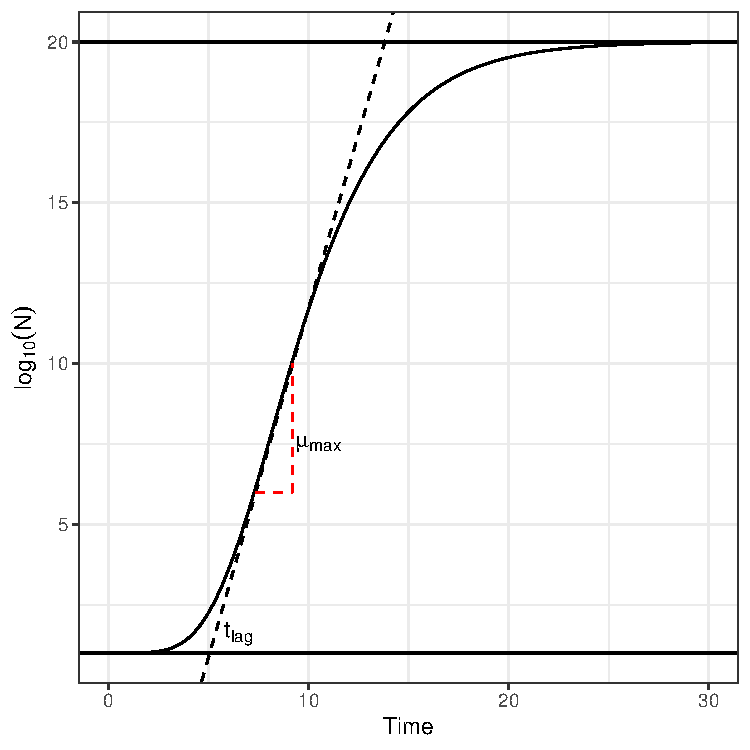
\includegraphics[width=4in]{../results/4_param_demo.pdf}
        \caption{Illustation of $\mu_{max}$ and $t_{lag}$ parameters. $\mu_{max}$ is the maximum gradient of the growth curve, and $t_{lag}$ is the intercept between this tangent line and the line $N = N_0$}
        \label{fig:4_param_demo}
        \end{figure}


        \begin{figure}[H]
        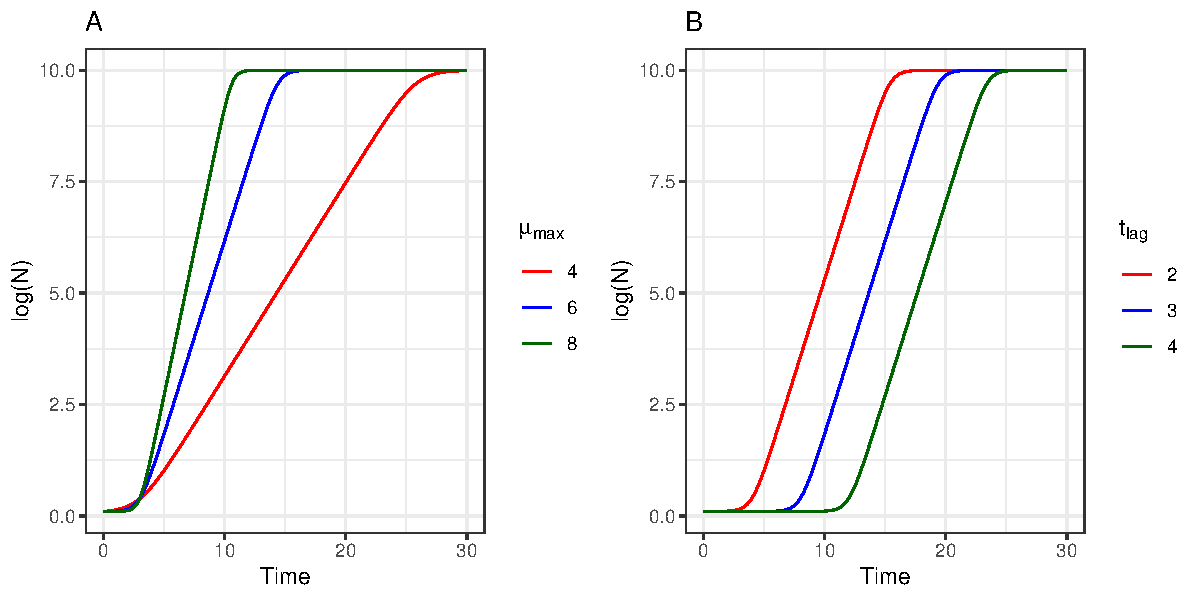
\includegraphics[width=\linewidth]{../results/tlag_rmax_demo.pdf}
        \caption{ $(A)\mu_{max}$ and (B) $t_{lag}$ parameters can be varied independently to control the rate of microbial growth, and the duration of the lag phase.}
        \label{fig:parameter_variation_demo}
        \end{figure}



\paragraph{Buchanan}
The Buchanan model \cite{Buchanan} is the simplest implementation of this, with a growth rate of zero during the lag and stationary phases, which surround a period of exponential growth:

  \[
    log(N_t) = \begin{cases}{}
        N_0 & \quad \text{if } t\leq t_{lag}\\
        N_0 + \mu_{max} \cdot (t - t_{lag}) &  \quad \text{if } t_{lag}\leq t\leq t_{max}\\
        N_{max} &  \quad \text{if } t\geq t_{max}
        \end{cases}
  \]

\paragraph{Gompertz}

The Gompertz model \cite{Gomp, zwitmodelling} describes a sigmoidal growth curve with a gradual transition into and out of the exponential phase. The Gompertz model has been popular for microbial population modelling, as it has empirically been found to fit well in a wide range of circumstances \cite{MicrobialGrowth}. However, it should be noted that its derivation does not have a mechanistic basis in microbial growth modelling \cite{EstBaranyi}, but rather in describing human mortality rates \cite{Gomp}. 

  \[log_{10}(N_t) = N_0 + (N_{max} - N_0)  e^{-e^{ \frac{\mu_{max} ~ \cdot ~ e  ~ \cdot ~ (t_{lag} - t)}{ (N_{max} - N_0) ~ \cdot ~ log(10)} + 1} }\]
  
  
\paragraph{Baranyi}

The Baranyi model is an attempt to formulate a truly mechanistic model for microbial population growth \cite{BaranyiOriginal, zwitmodelling}, explicitly modelling the internal physiological state and external environmental conditions of the cell. This produces a more flexible model, which can be applied to model population growth curves in time-varying environmental conditions. Here,  we use a version of the model in which conditions are homogenous, with the curvature parameter into the exponential phase $\nu$ set to $\mu_{max}$, and curvature parameter out of the exponential phase $m$ set at an empirical estimate of 1:

\[ log_{10}(N_t) = N_{max} + log_{10}(\frac{-1 + e^{\mu_{max} \cdot  t} + e^{\mu_{max} \cdot t_{lag}  } }{ -1 + e^{\mu_{max} \cdot t}  + e^{\mu_{max} \cdot t_{lag}} \cdot 10^{N_{max}-N_0}}) \]


        \begin{figure}[h]
        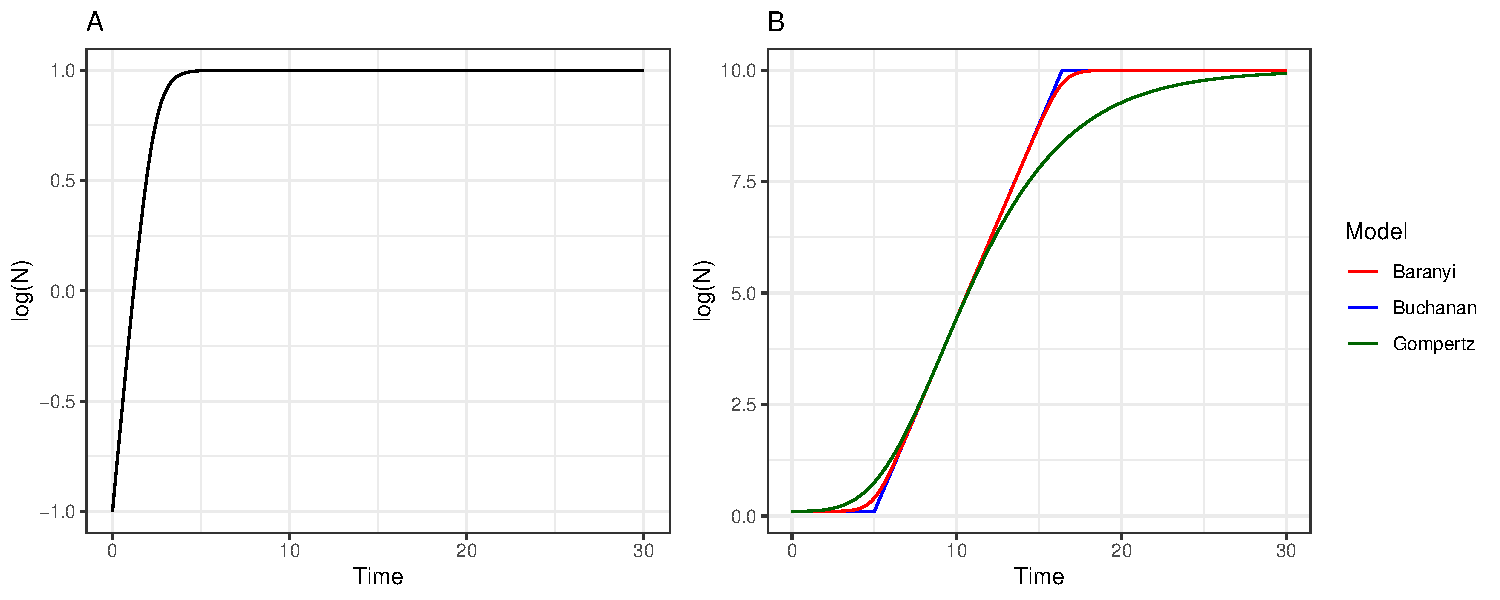
\includegraphics[width=\linewidth]{../results/model_demo.pdf}
        \captionsetup{format=hang}
        \caption{Demonstration of the shape of the 4 mechanistic models, plotted in log space. The logistic model (A) immediately starts growing at its maximum growth rate, whilst the three four-parameter models (B) have growth phases that transition into the exponential phase}
        \label{fig:models_demo}
        \end{figure}

\subsection{Phenomenological models}
As controls, I decided to fit quadratic and cubic polynomials to the data:
\paragraph*{Quadratic} $ N_t = at^2 + bt + c $
\paragraph{Cubic} \quad \quad $ N_t = at^3 + bt^2 + ct + d $


   \section{Methods}
   
   \subsection{Data}
   
\paragraph{Data sources}
The provided microbial growth data contained 305 time series, digitised from graphs in 10 papers from the microbial growth literature. The data set contained time series from 47 different species, 18 media, and 17 temperatures, with population size measured in 4 different units. However, the data from one citation \cite{discarded} clearly had incorrect time values, with times extending to 13,000 hours. I removed the data from this citation as there was not a clear correct transformation to produce the correct times, leaving 287 time series for analysis.

\paragraph{Log transformation}
As explained below, I decided to fit the model to $log_{10}(N)$ as well as to linear data. In 5/287 data sets, there were negative population counts due to numerical error in growth curve digitization. One value of approximately -668 was removed, whilst other negative values were greater that -10\textsuperscript{-2}; in these cases, I transformed increased population sizes for that time series by the minimum population size in the time series, discarding the minimum value of 0 before taking the logarithm.  

\paragraph{Time transformation}
I transformed each time series to start at $t = 0$ when fitting the four-parameter models, as model fits were clearly suboptimal without this transformation. Since $t_{lag}$ directly transforms the curve along the t-axis, $t_{lag}$ could be adjusted back to obtain model parameters which fit the untransformed time series. 

\subsection{Model Fitting}
When fitting the models, I used a least squares approach, both to log\textsubscript{10} transformed data, and to the original linear data (Figure \ref{sup:compare_least_squares}). This required exponentiating the four-parameter models to predict linear population size, and taking the logarithm of the logistic model to predict logarithmic population size. As such, the parameters of the four-parameter models remained in logarithmic space, and the parameters of the Logistic model in linear space. 

Due to the advantages presented in Results, I analysed parameter estimates from the log-fitted models (although linear fit results are presented in the Supplementary Figures), also choosing not to linearise residuals as this resulted in non-sensical fits (demonstrated in Figure \ref{sup:compare_least_squares}). These fits can be explained by the fact that, in general:
\[log(f(x) ) \neq f(log(x))\]
This means minimising errors in logarithmic space does not result in minimised errors in linear space, so evaluating fit in linear space does not capture the best possible fit for each model, (Figure \ref{sup:compare_least_squares}).

\subsubsection{Fitting linear models}

The two polynomial phenomenological models are linear in their parameters, so were fitted using Ordinary Least Squares with the lm() function in R \cite{R}.

\subsubsection{Fitting non-linear models}

The mechanistic models are non-linear, so are fitted using an optimisation approach. The nlsLM function in the minpack.lm \cite{minpack} package uses the Levenberg-Marquardt algorithm to optimise initial values to determine best fitting parameter values for a specified model. If initial values are far from the optimal parameters, it is likely that the optimisation will not converge, or will converge to very suboptimal parameters. It is therefore important to estimate reasonable starting values.

\paragraph{Estimating parameter values}
N\textsubscript{min} and N\textsubscript{max} were set as the minimum and maximum observed population size respectively. $\mu_{max}$ and $t_{lag}$ estimates were determined using a rolling regression (Figure \ref{sup:rolling_regression}), which computed the regression line for all sets of 5 adjacent data points. The regression line with the greatest gradient was selected, with the gradient taken as an estimate of $\mu_{max}$, and the $t$ value at the intercept between this regression line and $N = \min(N)$ taken as the $t_{lag}$ estimate. This was repeated in both logarithmic and linear space to provide parameter values for Logistic and four-parameter models.


\paragraph{Multiple fit attempts}
Despite well chosen initial values, models often fail to converge, or converge to poorly fitting parameter values. To increase the proportion of models which fit, and ensure that I find parameter values nearer the global optimum, I used a grid search to explore a range of initial parameter values. For each parameter, I chose linearly spaced samples from a range surrounding the estimate of that parameter value, and fitted a model for every combination of these parameter values. For example, if I take 3 samples for each of $N_0$ and $N_{max}$, and 5 for $t_{lag}$ and $\mu_{max}$, I fit $3 \times 3 \times 5 \times 5 = 225$ models. From the model fits that converge, I select the model with the smallest RSS. If none converge, I randomly sample parameter values with normally distributed noise around my parameter estimates until a model fits, or until there have been 1,000 failed attempts. 

Using this method, I was able to fit all 287 data sets for the Logistic, Gompertz, and Baranyi models in both linear space and logarithmic space. In linear space, there was one failed fit for the Buchanan model, and in log space there were two failed fits for the Buchanan model.


\subsection{Filtering}
Some data sets show no pattern of population growth, or have too few points in the growth phase to constrain the $mu_{max}$ and $t_{lag}$ parameters. I visualised the 64 data sets with the lowest maximum R\textsuperscript{2} value, removing 20 with no meaningful growth pattern or visibly little constraint (Figure \ref{sup:removed_ids}). For parameter estimate analysis, I further filtered out datasets with fewer than 2 points in the growth phase (Figure \ref{sup:constraint}) by counting the number of points with a time value within the predicted exponential phase, as determined using Akaike weighted parameter values. This removed a further 57 data sets, leaving 210 data sets.


\subsection{Model Selection}

Model fit was assessed using AIC \cite{AIC} and BIC \cite{BIC}. With the assumption of normally distributed errors, and simplification to remove constants, these are:
\[\text {AIC}  = 2k + n\log(RSS)\]
\[\text {BIC} = n\log{\frac{RSS}{n}} + k\log{n}\]


Both AIC and BIC balance fit against model complexity, allowing direct comparison of fit for models with differing numbers of parameters. However, BIC has the disadvantage of making a number of unrealistic assumptions about the true model: that it exists, is in the model set, and has equal prior probability to other models. Additionally, the fact that AIC is based in Kullback–Leibler information theory means that standardised model likelihoods - Akaike weights - can be calculated to naturally compare model support and allow model averaging \cite{Omland, ModelSelection}.


\subsection{Parameter Estimation}

Parameter estimation was performed using Akaike weights, which produce a single parameter estimate from a family of models \cite{ModelSelection}, weighted by the model’s relative likelihood.
With $\text{AIC}_{best}$ being the lowest observed AIC values for a dataset, $\Delta_{AIC}$ values are calculated with:
\[ \Delta_i = \text{AIC}_i - \text{AIC}_{best} \]

The Akaike weight for the $i^{th}$ model is then:
\[ w_i = \frac{e^{-\frac{1}{2}\Delta_i }} { \sum_{r = 1}^{r = R}  e^{- \frac{1}{2}\Delta_r }}\]

The Akaike weighted parameter estimate for $\theta$, with weights $w_i$ and individual model parameter estimates $\theta_i$ is:
\[\theta_w = \sum_{i = 1}^{i = I}\theta_i * w_i\]


\subsection{Statistical Analysis}

I ran linear regressions of $\Delta_{\text{Logistic - Gompertz}}$ against temperature, and $\Delta_{\text{Logistic - Gompertz}}$ against proportion of points in the lag phase, using lm() in R \cite{R}. Their diagnostic plots were examined to confirm the suitability of a linear model.

I ran a mixed effects model of $\mu{max}$ against temperature, and of $t_{lag}$ against temperature, with species and medium used as random effects in each case. Again, diagnostic plots were used to confirm that residuals were homogeneous across the fitted values.

I ran a paired t-tests for $\mu_{lag}$ and $t_{lag}$ between the each pair of four-parameter models, and between linear and logarithmic space fits, to check for systematic differences in parameter estimates. I check for normality of differences by plotting histograms of these differences.  

\subsection{Computing Tools}
\paragraph{R 3.6.1 \cite{R}} was used for initial data preparation script, model fitting, analysis, and figure preparation. R was chosen because the native data structures are naturally suited to this type of data, and support of vectorised operations makes the code cleaner than it would be in Python. I used R for my multi-start method to fit models over a range of initial parameter values because of the efficiency of non-linear least squares model fitting in the minpack.lm package. \textbf{minpack.lm \cite{minpack}} was used for non-linear least squares model fitting using the more robust Levenberg-Marquardt algorithm (relative to Gauss-Newton). \textbf{ggplot2 \cite{gg}} was used to create high quality graphics. \textbf{dplyr \cite{dplyr}} was used for data wrangling. \textbf{lme4 \cite{lme4}} was used to fit linear mixed models. \textbf{toOrdinal \cite{tO}} was used for annotations.

\paragraph{Python 3.7.4 \cite{python}} was used for calculation of initial values. \textbf{pandas \cite{pd}} was used for dataframes in Python. \textbf{matplotlib \cite{plt}} was used to create graphics in Python. \textbf{SciPy \cite{numpy}} was used to fit linear regressions for the rolling regression. \textbf{NumPy \cite{numpy}} was used for efficient arrays.

\paragraph{bash 3.2} was used to write scripts tying other elements of the project together.

\paragraph{\LaTeX } was used for compilation of this write-up.
\section{Results}

\subsection{Model fitting is highly successful}
Taking the best fitting model from a range of initial parameter values was very effective, with all models converging to every data set when those with no discernible growth pattern were removed, and only 3 unsuccessful fits otherwise (2293 / 2296 successful non-linear fits overall). Model fits were visually inspected, and found to describe the data well (Figure \ref{fig:model_fits} for logarithmic fits, Figure \ref{sup:model_fits_linear} for linear fits). For the reasons expanded on in the Discussion, I present the results obtained from fitting models in logarithmic space first, before examining the results from linear space fits at the end of this section.

         \begin{figure}[H]
         \centering
       	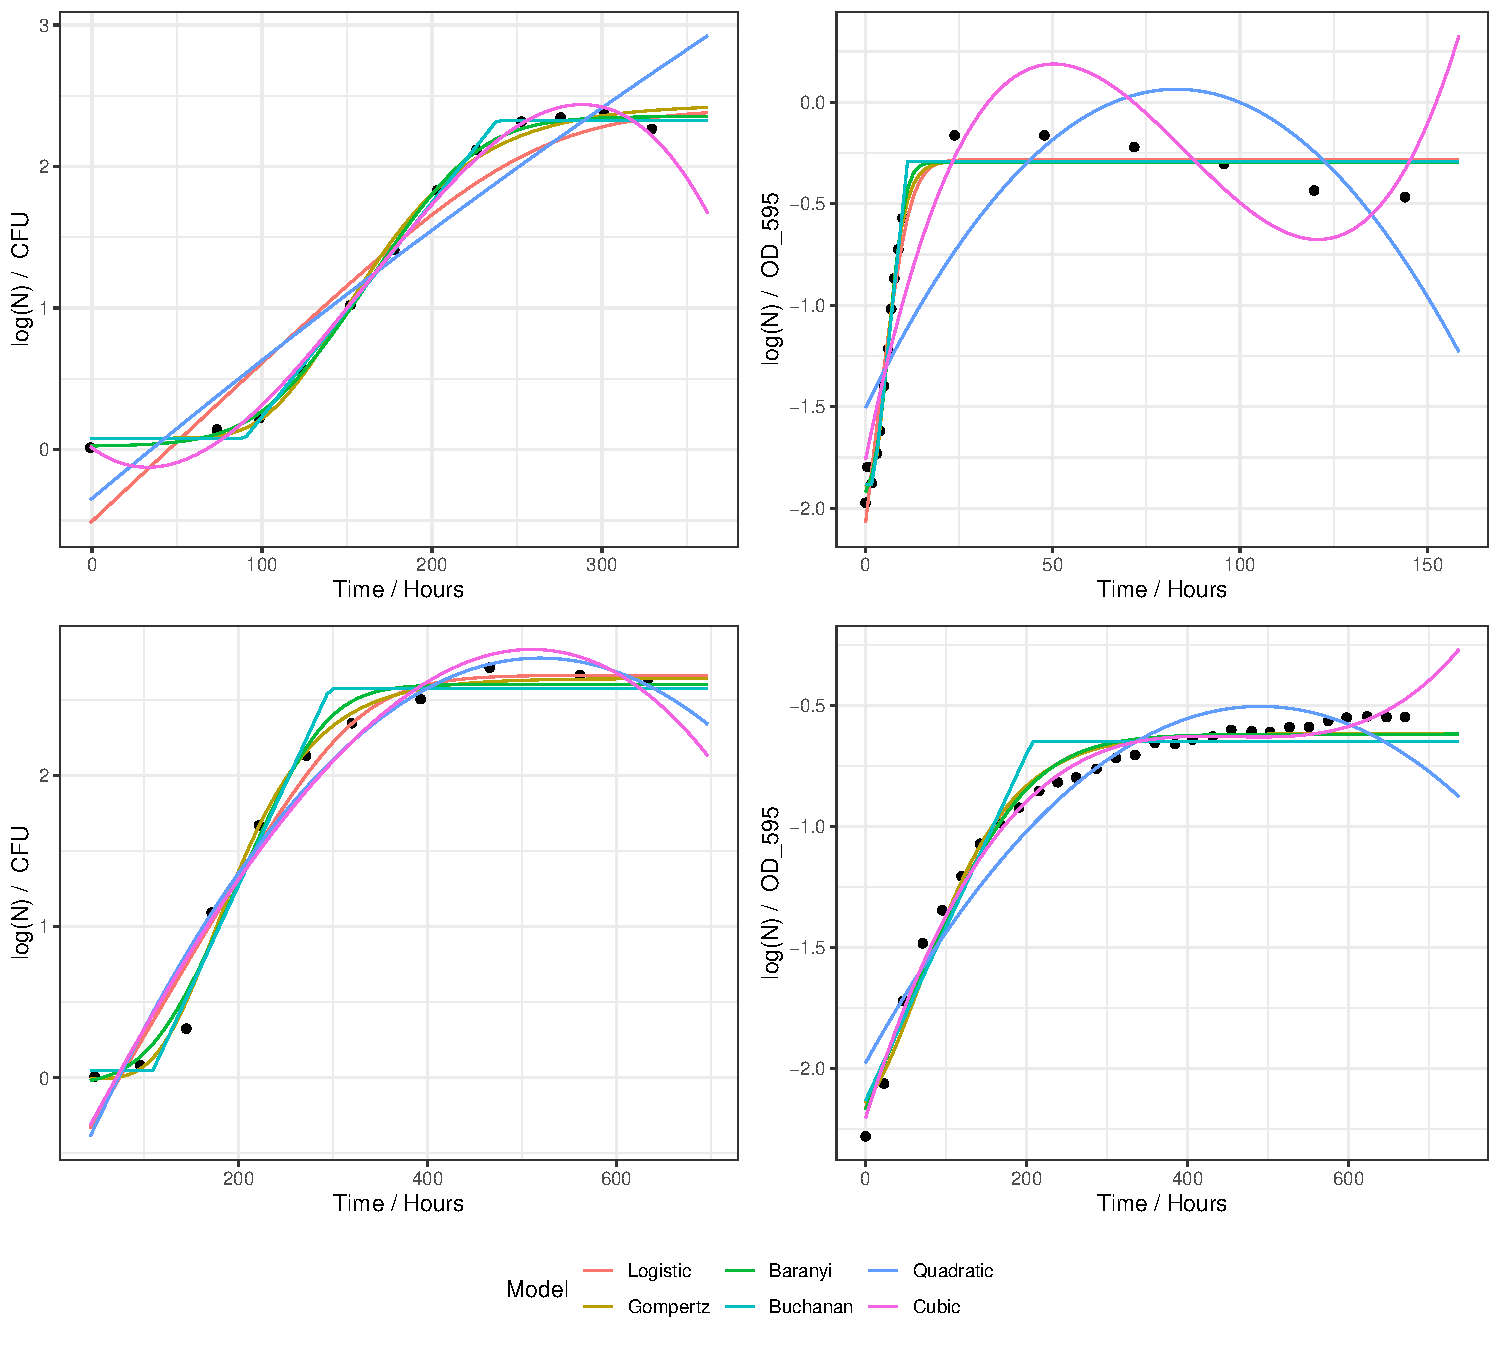
\includegraphics[height=4.5in]{../results/model_fits.pdf}
        \caption{Demonstration of model fits in log space. Out of 287 data sets, all fits were successful apart from two fits of the Buchanan model, to datasets which were removed anyway. }
        \label{fig:model_fits}
        \end{figure}

\subsection{Gompertz and Baranyi are best supported}

The Gompertz model and Baranyi model are both well supported by the data. The Gompertz model most frequently has the lowest AIC (Figure \ref{fig:bestbars} A), and has the highest mean Akaike weight (Figure \ref{AWdist} and Table \ref{tab:meanAICBIC}). However, the Baranyi model has a lower mean ranking (Figure \ref{fig:bestbars} C), and lower mean AICs and BICs. (Table \ref{tab:meanAICBIC}). It appears that the Baranyi model is a consistent good fit to the data, achieving the lowest mean AIC despite relatively rarely being the best fitting model - as evidenced by it placing second for nearly half of the datasets (Figure \ref{fig:bestbars} B).



        \begin{figure}[H]
        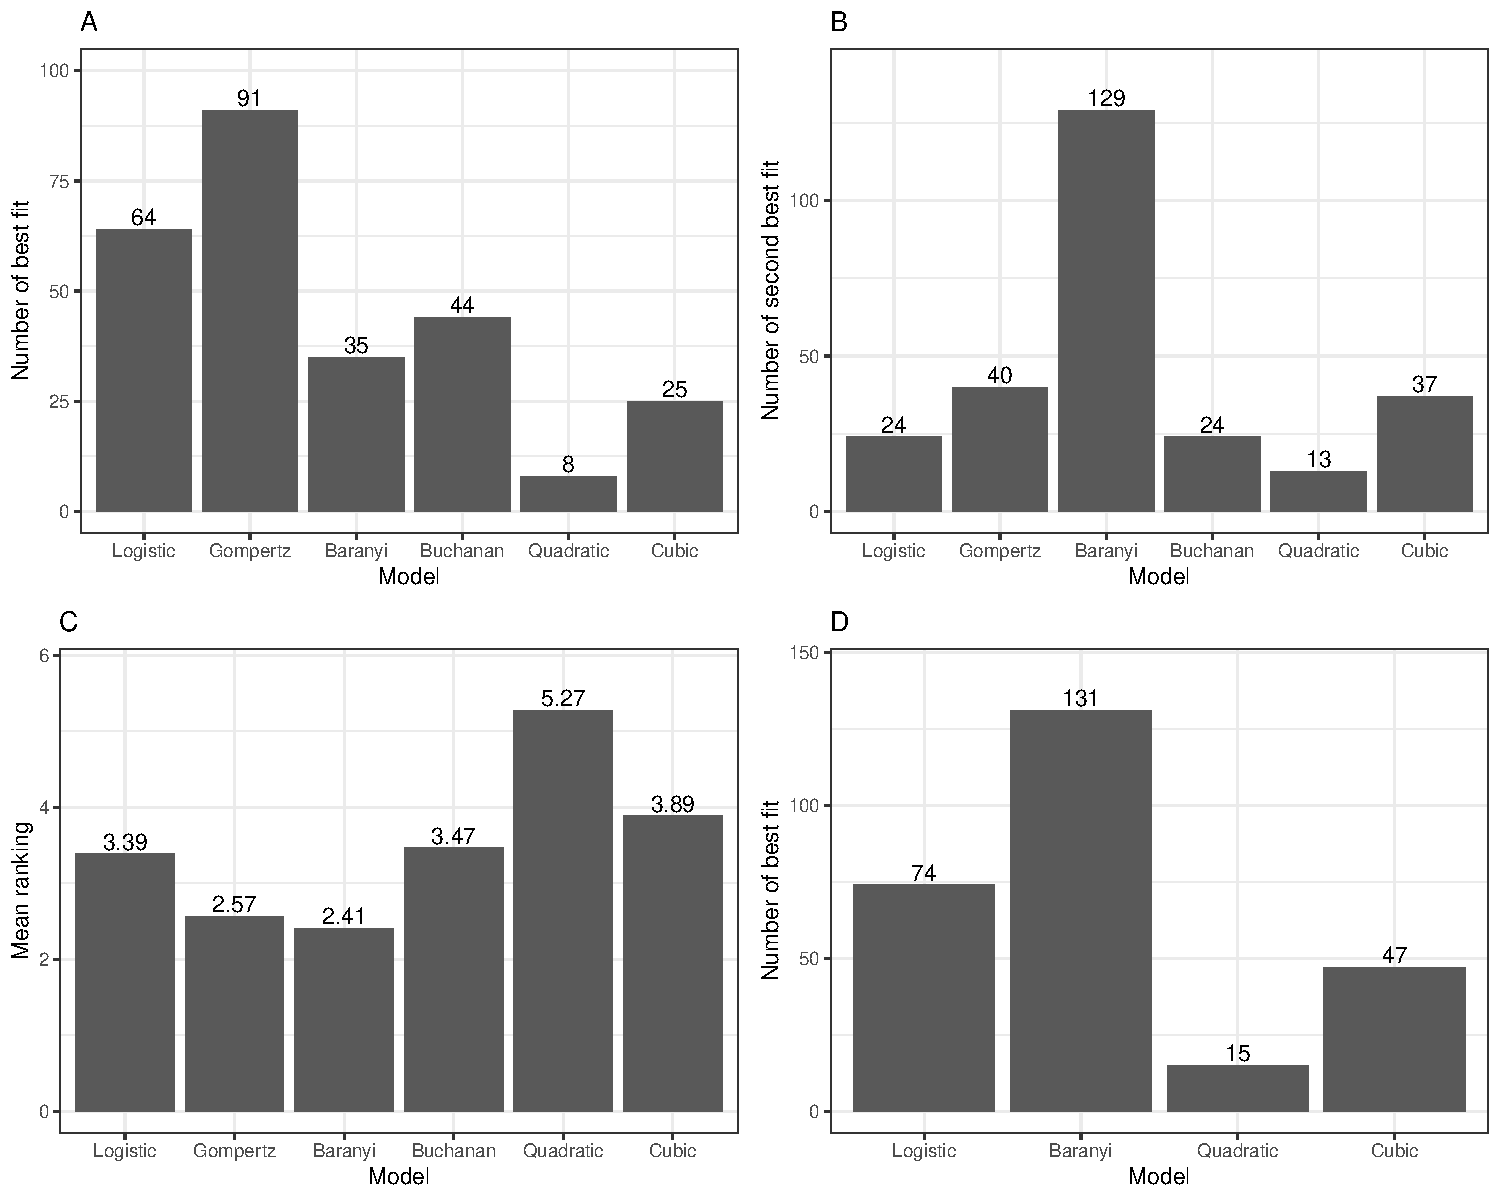
\includegraphics[width=\linewidth]{../results/best_fit_frequency_bar.pdf}
        \caption{Plots showing the rankings of models in logarithmic space. (A) shows the number of times each model is the best fitting model for a dataset. (B) shows the number of times each model is the second best fitting model for a dataset. (C) shows the mean ranking for each model. (D) shows the number of times each model is the best fitting model for a dataset if we do not consider the Gompertz and Buchanan models. }
        \label{fig:bestbars}
        \end{figure}
        
         \begin{table}[H]
	\centering
	\begin{tabular}{l|llllll}
       & Logistic & Gompertz & Baranyi & Buchanan & Quadratic & Cubic \\ \hline
AIC & -58.5    & -66.2    & -66.3   & -61.1    & -43.7     & -53.2 \\
BIC & -57.0    & -64.1    & -64.2   & -59.1    & -42.2     & -51.1 \\
$A_w$ & 0.162     & 0.316     & 0.218   & 0.156     & 0.0319     & 0.116
	\end{tabular}
	\caption{Mean AIC, BIC, and A\textsubscript{w}  values for each model, fitted in logarithmic space. Lower AIC represents greater relative support, whilst higher $A_w$ represents greater relative likelihood.}
	\label{tab:meanAICBIC}
	\end{table}




        \begin{figure}[H]
        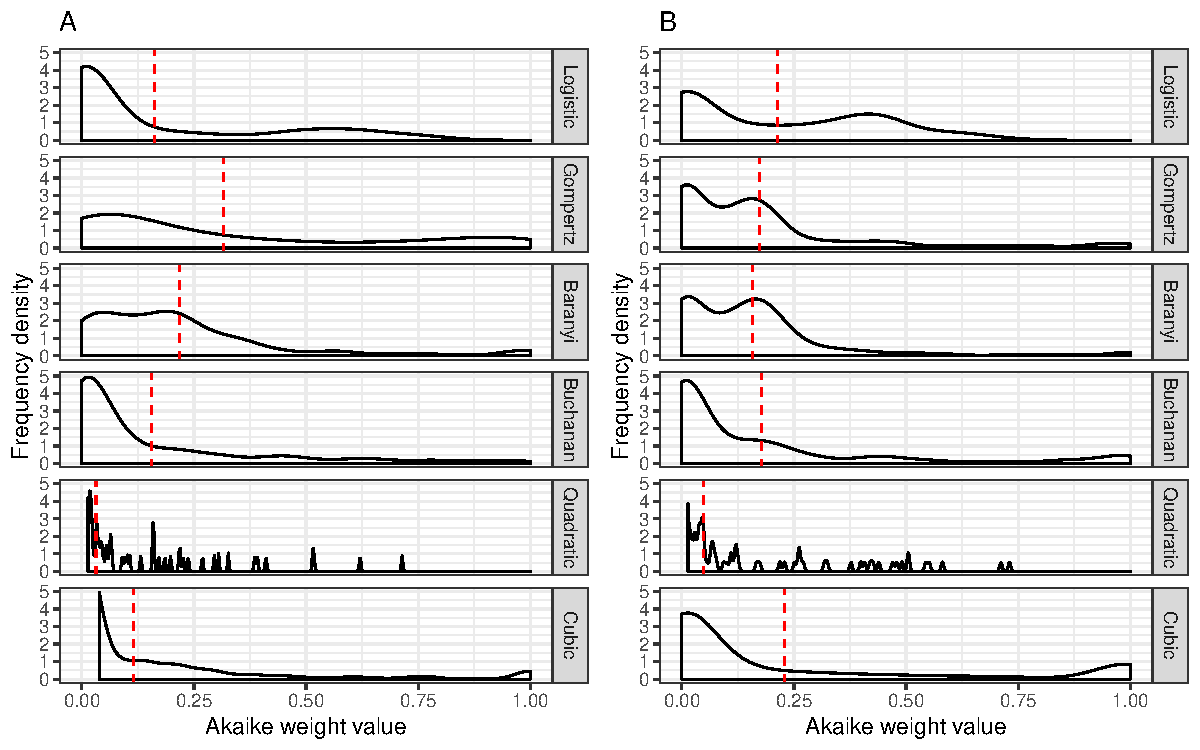
\includegraphics[height=3.5in]{../results/Aw_distributions.pdf}
        \caption{Gaussian Kernel Density Estimates for Akaike weights in logarithmic (A) and linear (B) space for each model. We see that in logarithmic space, the Gompertz model has strongest support, with the Logistic model have highly variable support due to its inability to model $t_{lag}$. In linear space, poor lag phase modelling is less strongly penalised, so the Logistic model gains the most support. }
        \label{fig:AWdist}
        \end{figure}
        
        

        
        \subsection{Logistic fit is poor when t\textsubscript{lag} is high}
                
        Notably, the Logistic model is the best model second most frequently despite its mean AIC and BIC scores placing fourth best - implying great variability in its performance. We can see this variability in its A\textsubscript{w} distribution, with high probability density near zero but a relative high density in the 0.5 to 0.75 interval (Figure \ref{AWdist}.  This can be explained by the absence of a lag phase in the model: the Logistic model fits poorly when a lag phase is present, but fits well when it is absent without incurring the AIC/BIC penalty for a fourth parameter. This is evident in the increasing proportion of points in the lag phase as the ranking of the logistic model gets worse (Figure \ref{fig:logistic_tlag} A). More explicitly, the difference in AIC between the Logistic and Gompertz model increases with proportion of data points in the lag phase (Figure \ref{fig:logistic_tlag} B). This relationship is strongly significant, with a linear regression estimating an increase in $\Delta_{\text{Logistic - Gompertz}}$ of 6.9 for every increase in lag phase proportion of 0.1, with a standard error of 0.47.
        
                \begin{figure}[H]
        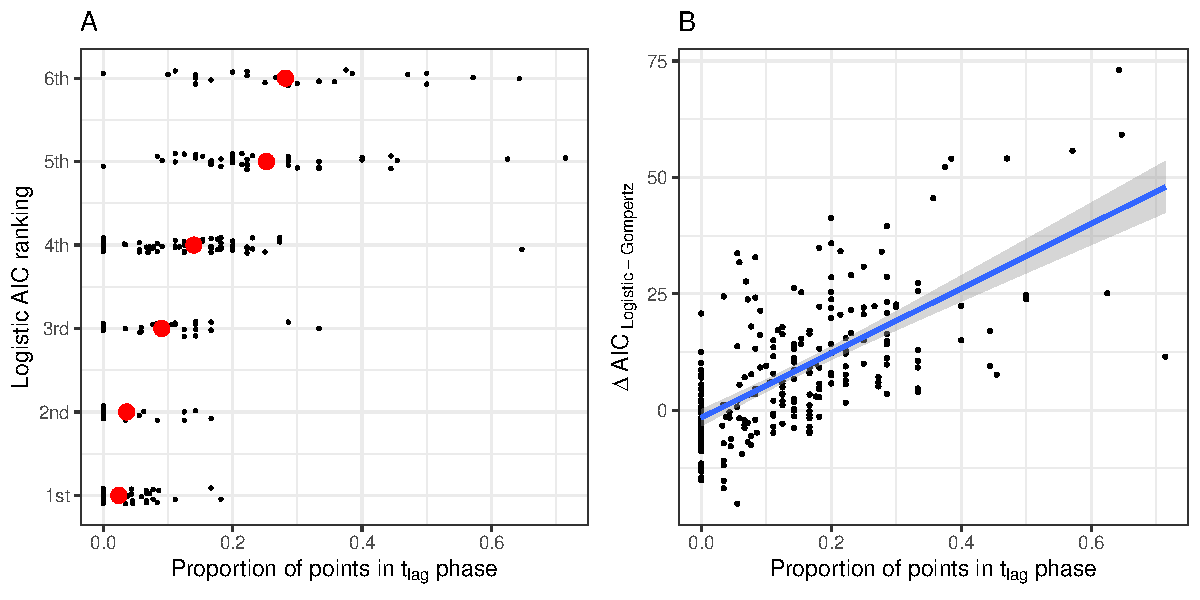
\includegraphics[width=\linewidth]{../results/tlag_vs_logistic.pdf}
        \caption{(A) is a plot of proportion of points in the lag phase, against the ranking of the Logistic model by AIC. We see that an increasing proportion of points in the lag phase is associated with a poorer ranking - with the mean proportion for each ranking shown by the red circle. (B) shows the difference in AIC score between the Gompertz and Logistic model against this proportion, with a statistically significant slope observed.}
        \label{fig:logistic_tlag}
        \end{figure}        
        
        \subsection{Temperature affects $\mu_{max}$ and $t_{lag}$}
        
         I ran a linear mixed model to determine the effect of temperature on $\mu_{max}$ and $t_{lag}$ across the entire data set, including species and medium as random effects. Temperature was included as a categorical variable as it is unlikely that the response to temperature is linear across the entire temperature range. From this, estimates for $\log(\mu_{max})$ and $t_{lag}$ values were be made for each temperature, shown in Figure \ref{fig:params_temp}. It is clear that the logarithm of the maximum rate of bacterial growth increases with temperature, approximately linearly across much of the temperature range, indicating an Arrhenius type thermal response. $t_{lag}$ decreases with temperature, quickly levelling off at around 10\degree C. 

         \begin{figure}[H]
        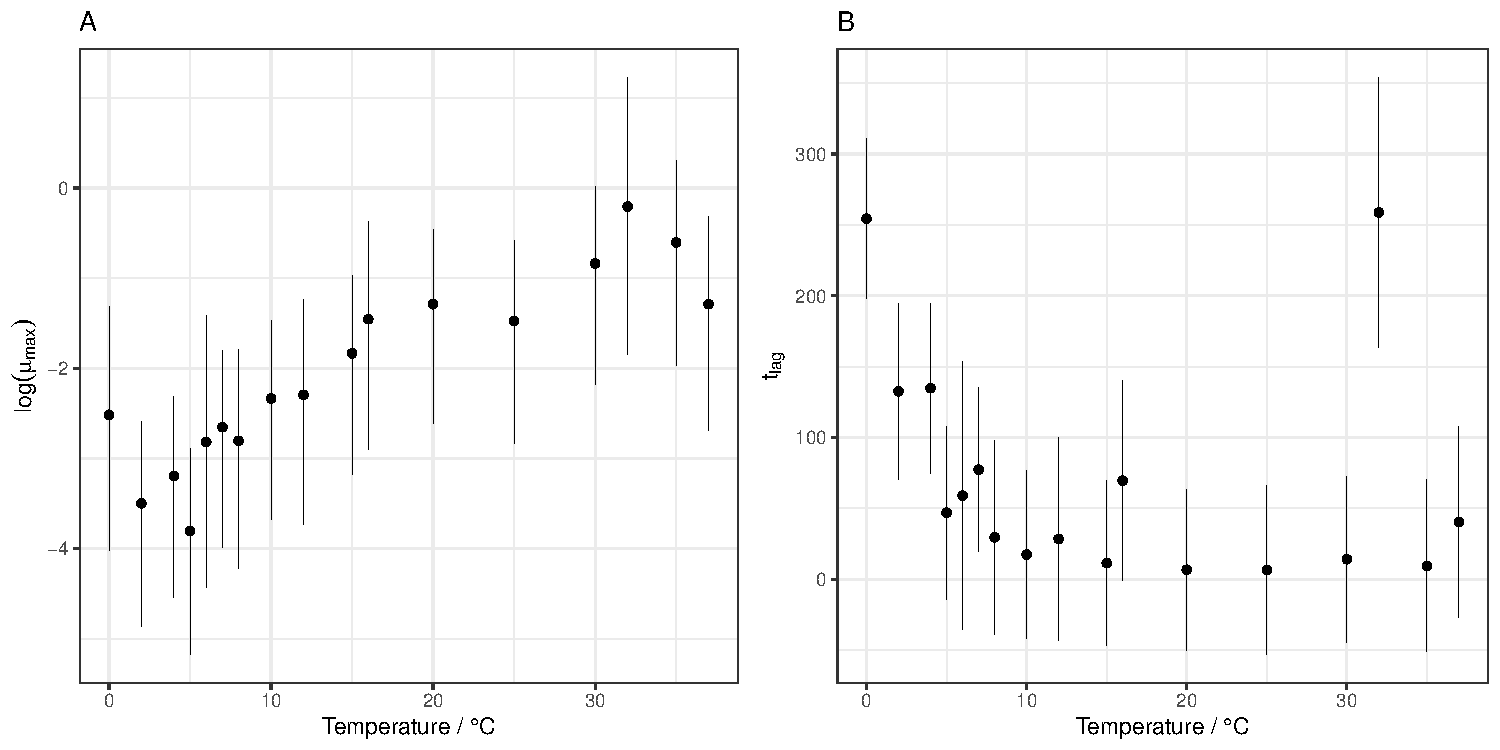
\includegraphics[width=\linewidth]{../results/tlags.pdf}
        \caption{(A) shows the relationship between $\mu_{max}$ and temperature, as estimated by a linear mixed model with temperature as a categorical variable. Vertical lines indicate the 95\% CI. $\mu_{max}$ increases steadily with temperature over the observed range. Similarly, (A) shows the relationship between $t_{lag}$ and temperature. We see that below 10\degree C, $t_{lag}$ increases rapidly as temperature decreases.   }
        \label{fig:params_temp}
        \end{figure}  



\subsection{Logistic model fits better at higher temperatures}

The decrease in $t_{lag}$ with temperature implies that the Logistic model, which has better fit with smaller $t_{lag}$, should have better fit with increasing temperature. Indeed, Figure \ref{fig:logistic_temp}A shows that $\Delta_{\text{Logistic - Gompertz}}$  decreases with increasing temperature. A linear regression suggests a decrease in $\Delta_{\text{Logistic - Gompertz}}$ of 3.30 for every 10\degree C, with standard error of 0.8.

        \begin{figure}[H]
        \centering
        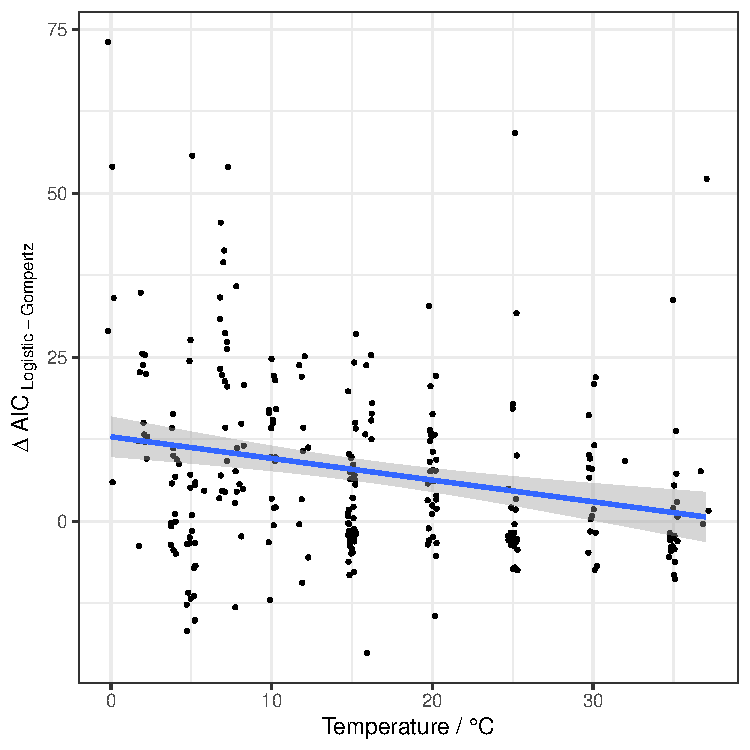
\includegraphics[width=4in]{../results/logistic_vs_gompertz_temp.pdf}
        \caption{$\Delta_{\text{Logistic - Gompertz}}$ is seen to decrease by 3.30 for every 10\degree C, indicating an improvement in the fit of the Logistic model relative to the Gompertz model as temperature increases.}
        \label{fig:logistic_temp}
        \end{figure}  

\subsection{Model choice biases parameter estimates}

Tables \ref{tab:tlag_biases} and \ref{tab:rmax_biases} show the mean pairwise differences in $t_{lag}$ and $\mu_{max}$ for the 4-parameter models. The Buchanan model results in the lowest $t_{lag}$ and lowest $\mu_{max}$ values. This is because the model assumes that population growth remains exactly at zero until $t = t_{lag}$, rather than smoothly transitioning to $\mu_{max}$ before this intercept. This means that Buchanan model fits must decrease $t_{lag}$ to capture the first part of the growth phase, consequently lowering $t_{lag}$ and $\mu_{max}$ values (Figure \ref{sup:fit_difference}).

\begin{table}[H]
\centering
\begin{tabular}{l|lll}
         & Gompertz                                        & Baranyi                                         & Buchanan                 \\ \hline
Gompertz & \cellcolor[HTML]{9B9B9B}                        & -5.21 = - 9.8\%                                           & 4.23 = 8.0\%                     \\
Baranyi  & \cellcolor[HTML]{9B9B9B}{\color[HTML]{9B9B9B} } & \cellcolor[HTML]{9B9B9B}{\color[HTML]{9B9B9B} } & 9.44 = 17.8\%                     \\
Buchanan & \cellcolor[HTML]{9B9B9B}{\color[HTML]{9B9B9B} } & \cellcolor[HTML]{9B9B9B}                        & \cellcolor[HTML]{9B9B9B}
\end{tabular}
\caption{Mean pairwise differences in $t_{lag}$ estimates for all models, and as proportions of the Akaike weighted mean $t_{lag}$ value. The value in $(i, j) = t_{lag}^i - t_{lag}^j$. The Buchanan model produces lower $t_{lag}$ estimates than either the Baranyi or the Gompertz models. All values are significant at the 5\% level.}
\label{tab:tlag_biases}
\end{table}


\begin{table}[H]
\centering
\begin{tabular}{l|lll}
         & Gompertz                                        & Baranyi                                         & Buchanan                 \\ \hline
Gompertz & \cellcolor[HTML]{9B9B9B}                        & -0.025 = -5.4\%                                           & 0.11 = 23.4\%                     \\
Baranyi  & \cellcolor[HTML]{9B9B9B}{\color[HTML]{9B9B9B} } & \cellcolor[HTML]{9B9B9B}{\color[HTML]{9B9B9B} } & 0.14 = 29.3\%                     \\
Buchanan & \cellcolor[HTML]{9B9B9B}{\color[HTML]{9B9B9B} } & \cellcolor[HTML]{9B9B9B}                        & \cellcolor[HTML]{9B9B9B}
\end{tabular}
\caption{Mean pairwise differences in $\mu_{max}$ estimates for all models, and as proportions of the Akaike weighted mean $t\mu{max}$ value. The value in $(i, j) = \mu_{max}^i - \mu_{max}^j$. The Buchanan model produces lower $\mu_{max}$ estimates than either the Baranyi or the Gompertz models. All values are significant at the 5\% level.}
\label{tab:rmax_biases}
\end{table}

\subsection{Model fitting in linear space fails to resolve the lag phase}
As discussed below, fitting the models to minimise linear RSS reduces the penalty for mischaracterising growth at small population sizes. The Logistic model is therefore favoured when fitting in linear space, despite its lack of a lag phase: it has the highest mean Akaike weight (Figure \ref{AWdist} B), is most frequently the best model, and has the lowest mean ranking (Figure \ref{sup:frequency_bar_linear} and Table \ref{suptable:meanAICBIClinear}). Further, the weakened penalisation of the lag phase means that the relationship between Logistic model fit and proportion of points in the lag phase is much weaker (Figure \ref{sup:logistic_temp_linear}), and the relationship with temperature becomes smaller and loses significance (Figure \ref{sup:logistic_temp_linear}). Finally, a paired t-test showed that fitting in linear space was associated with a reduction in the $t_{lag}$ parameter of 6.11 relative to logarithmic space, although with a 95\% CI extending from 0.53 to 11.70.



\section{Discussion}
\subsection{Mechanistic modelling is limited in its resolution between biological hypotheses}
The results are unequivocal about the importance of a lag phase for modelling microbial growth in logarithmic space, with the four-parameter models having the most support by Akaike weights, AICs, and BICs. Further, the fit of the Logistic model worsens with increasing lag phase duration. However, the difference in mean AIC between the Gompertz and Baranyi model is negligible, so no concrete mechanistic statements can be made - especially given that the Gompertz model is only mechanistic to the extent that it models the three canonical phases of the growth curve. Indeed, it has been argued that mechanistic modelling of this sort cannot strongly discern between biological hypotheses, which should be confirmed by direct observation or experimentation rather that argumentation about the cause of differences in model fit \cite{MicrobialGrowth}. Indeed, direct observation of the process of microbial growth can also provide us with estimates of parameters such as $t_{lag}$ and $\mu_{max}$ which currently have caveats in their interpretation, by directly counting and timing cell divisions. However, for parameter estimation and prediction in its current form, I propose that the Baranyi model is a stronger choice:

\begin{enumerate}
\item{Consistency: }
The Baranyi model is a more consistently good fit, achieving a marginally lower AIC despite rarely being the best fitting model. This implies that the Baranyi model can be deployed ore broadly and reliably than the Gompertz model, and that parameter estimates are likely to be more consistent.

\item{Truly mechanistic: }
The Baranyi model has the advantage that it was formulated entirely with microbial growth in mind, giving it a more mechanistic basis in microbial growth modelling, and therefore more interpretable parameters. The full Baranyi model also has extra curvature parameters $\nu$ and $m$, which alter the transition into and out of the exponential phase. As more data becomes available, these parameters can be estimated to form a more detailed understanding of the mechanisms behind microbial growth. Similarly, the Baranyi model's capacity to make predictions with non homogenous environmental conditions in its differential equation form makes it a much more flexible tool for growth modelling. 

 \end{enumerate}

\subsection{Lowering temperature can significantly impede microbial growth}

I find that $\log(\mu_{max})$ increases roughly linearly with temperature, corresponding to an exponential increase in $\mu_{max}$. Similarly, I find that $t_{lag}$ decreases rapidly with increasing temperature, such that the advantage of lower temperatures is almost entirely lost by 10 \degree C. Clearly, minimising the temperature of food storage can have a dramatic effect in decreasing microbial load - and conversely, increasing the temperature can result in growth orders of magnitude faster, with perhaps even brief exposure to higher temperatures able to spoil food. It will therefore be important to see how microbial growth patterns respond to temperatures that vary over time, which the Baranyi model will be very helpful in studying.

\subsection{Parameter biases necessitate caution in meta-analyses}

There is a clear hierarchy in the magnitude of parameter estimates from the three models. The Buchanan model produces the lowest $t_{lag}$ and $\mu_{max}$ estimates, with the Baranyi producing the highest, and Gompetz producing intermediate values. The magnitude of the differences between the Buchanan and Baranyi model reach 29\% of the Akaike weighted estimate for $\mu_{max}$, and 17\% for $t_{lag}$. These are extremely significant differences, so great care, probably involving reevaluation of raw data sets, is needed to ensure that parameter estimates from different sources are meaningfully compared, such that these biases are not interpreted as biological effects. A simulation study could be used to determine which model, or combination of models, produces the most reliable parameter estimate. Datasets produced by a variety of simulation mechanisms, with known 'true parameters' could be produced for a range of generative processes, and used to test how robust each of the models is to deviations from their mechanistic assumptions, and to noise in the data.

\subsection{Fitting in logarithmic space is required to estimate relevant parameters}
When fitting in linear space, the logistic model is most supported. This is a strong remit to recommend that logarithmic space should be used, as the success of the Logistic model demonstrates that linear space fitting only weakly enforces accurate modelling of the lag phase. As linear space fitting is concerned with modelling absolute, rather than relative, population size, mischaracterisation of the early growth phase is not strongly penalised. The ability to describe the lag phase as the early stage of population growth also leads to systematically lower $t_{lag}$ estimates when fitting in linear space. Fitting in logarithmic space is therefore strongly recommended for food preservation work, where early growth curve behaviour is of centrally interest as food is often spoiled before $N_{max}$ is reached \cite{MicrobialGrowth}.

As such, this study has demonstrated that the choice of space and model in microbial growth modelling can have profound effects both on parameter estimates, and may even even conceal findings. Further work examining the reliability of the various models to violations of their assumptions is needed to devise strategies that can provide the most accurate parameter estimates, which will allow increasingly quantitative approaches to food preservation.


\end{linenumbers}

\section{Supplementary Material}
\beginsupplement

        \begin{figure}[H]
        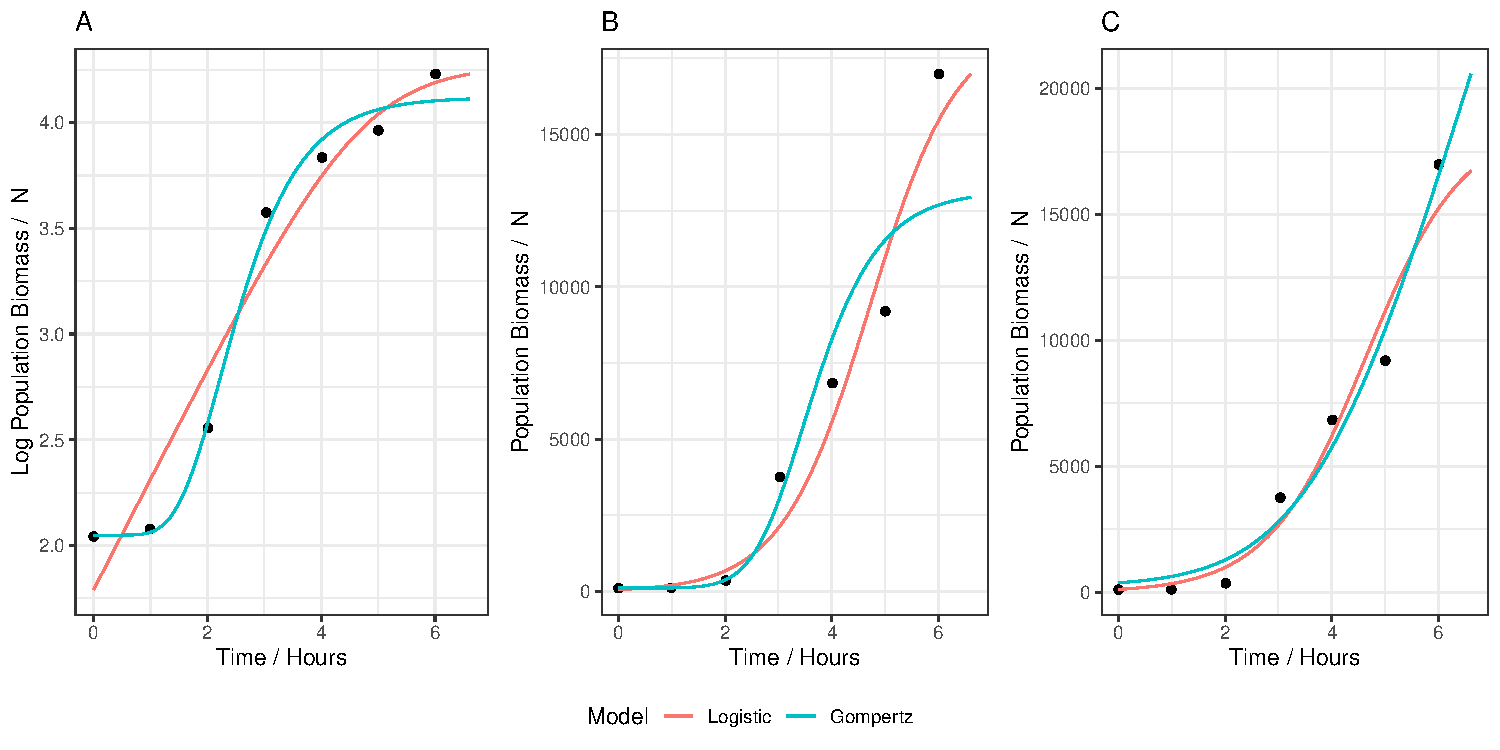
\includegraphics[width=\linewidth]{../results/compare_log_lin_fit.pdf}
        \captionsetup{format=hang}
        \caption{Comparison of: (A) fitting and evaluating modelling in log space. (B) fitting model in log space, evaluating fit in linear space. (C) fitting and evaluating model in linear space. \newline When the models are fit and evaluated in log space, it is clear that the Gompertz model has a better fit. However, if evaluation is done in linear space of these fits, the logistic model appears to have a better fit. This is shown to be invalid, as fitting the models in linear space demonstrates that the Gompertz model can in fact achieve better fits in both spaces.  }
        \label{sup:compare_least_squares}
        \end{figure}
        
        
        \begin{figure}[H]
        \centering
        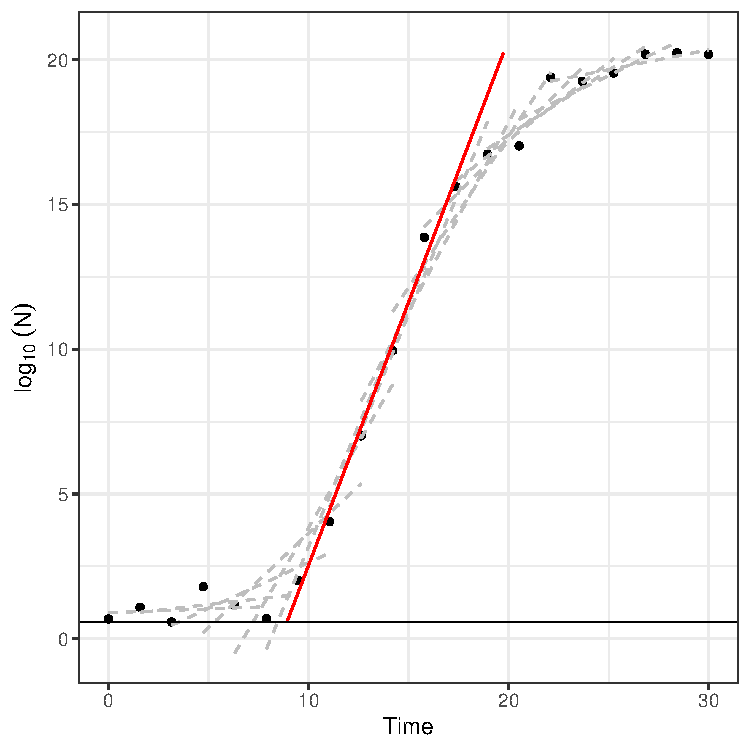
\includegraphics[width=3.5in]{../results/rolling_reg.pdf}
        \caption{Rolling regression was used to produce starting parameters. The regression line with the greatest gradient was selected, with its gradient used as $\mu_{max}$, and its intercept with $N = \min(N)$ used as $t_{lag}$ }
        \label{sup:rolling_regression}
        \end{figure}  
        
        
         \begin{figure}[H]
        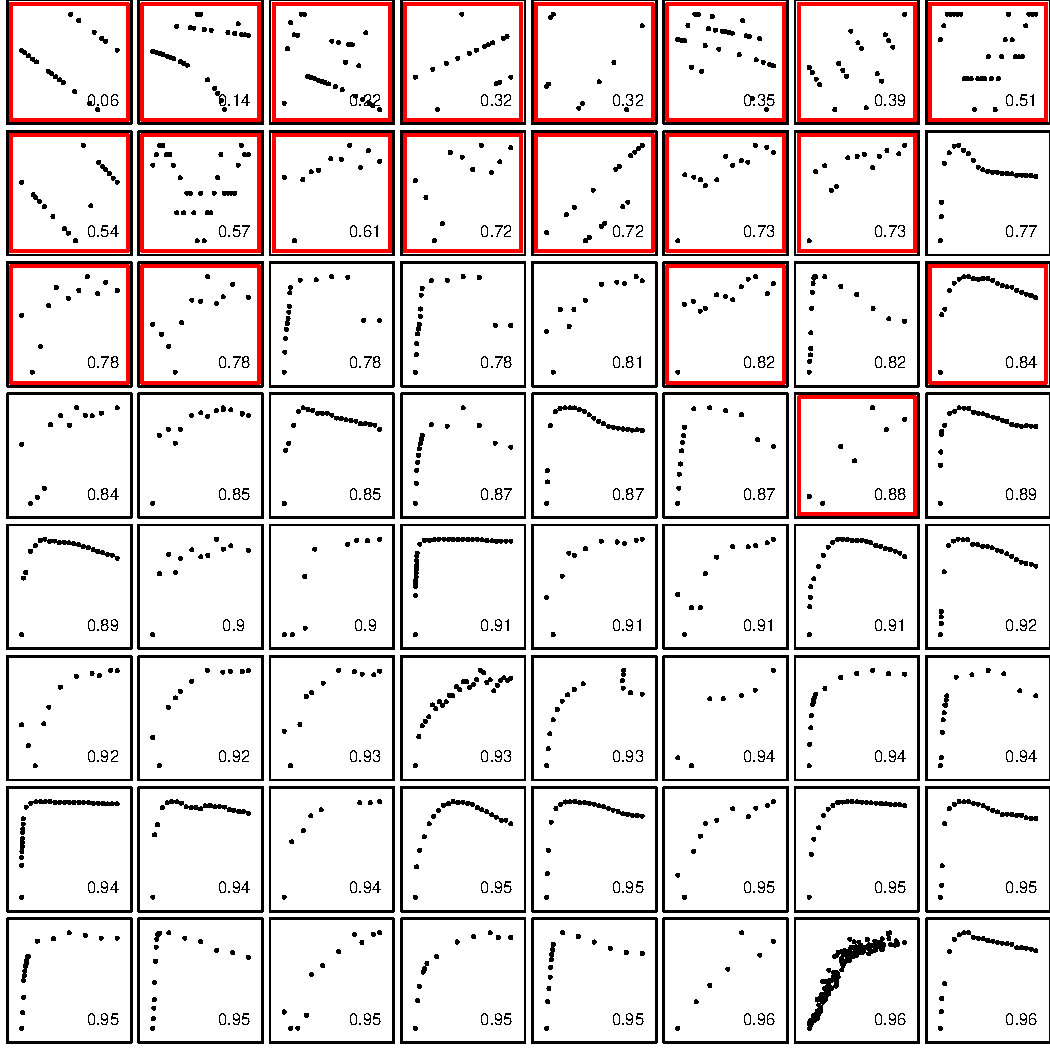
\includegraphics[width=\linewidth]{../results/removed_ids.pdf}
        \caption{The 64 datasets with the lowest maximum R\textsuperscript{2}. Those which were manually removed are highlighted with a red border.}
        \label{sup:removed_ids}
        \end{figure}
        
         \begin{figure}[H]
        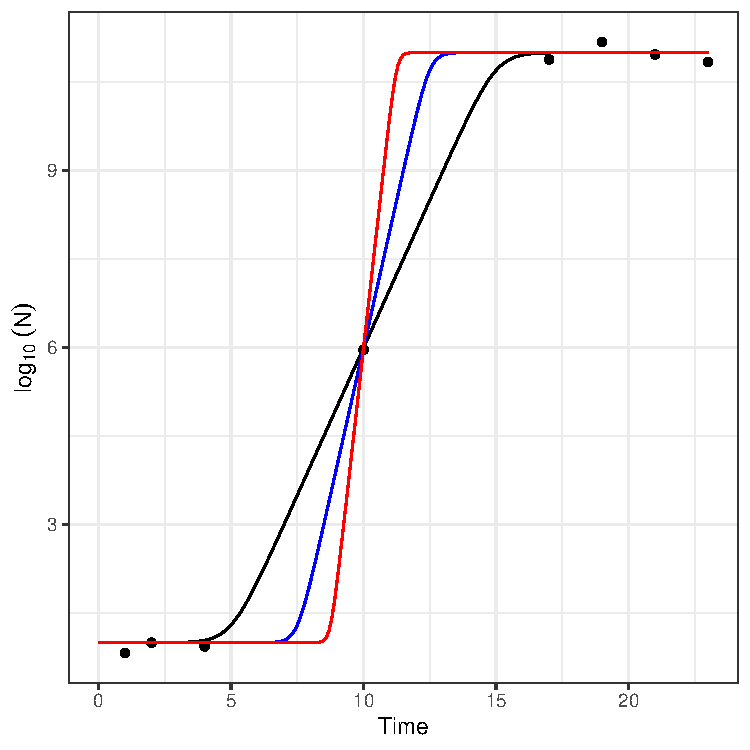
\includegraphics[width=3.5in]{../results/constraint_demo.pdf}
        \centering
        \caption{If there are too few points in the growth phase, $\mu_{max}$ and $t{lag}$ will not be well constrained. Here, we can see that there are infinitely many solutions that can fit equally well to the data as there is only one point in the growth phase. }
        \label{sup:constraint}
        \end{figure}  


         \begin{figure}[H]
         \centering
        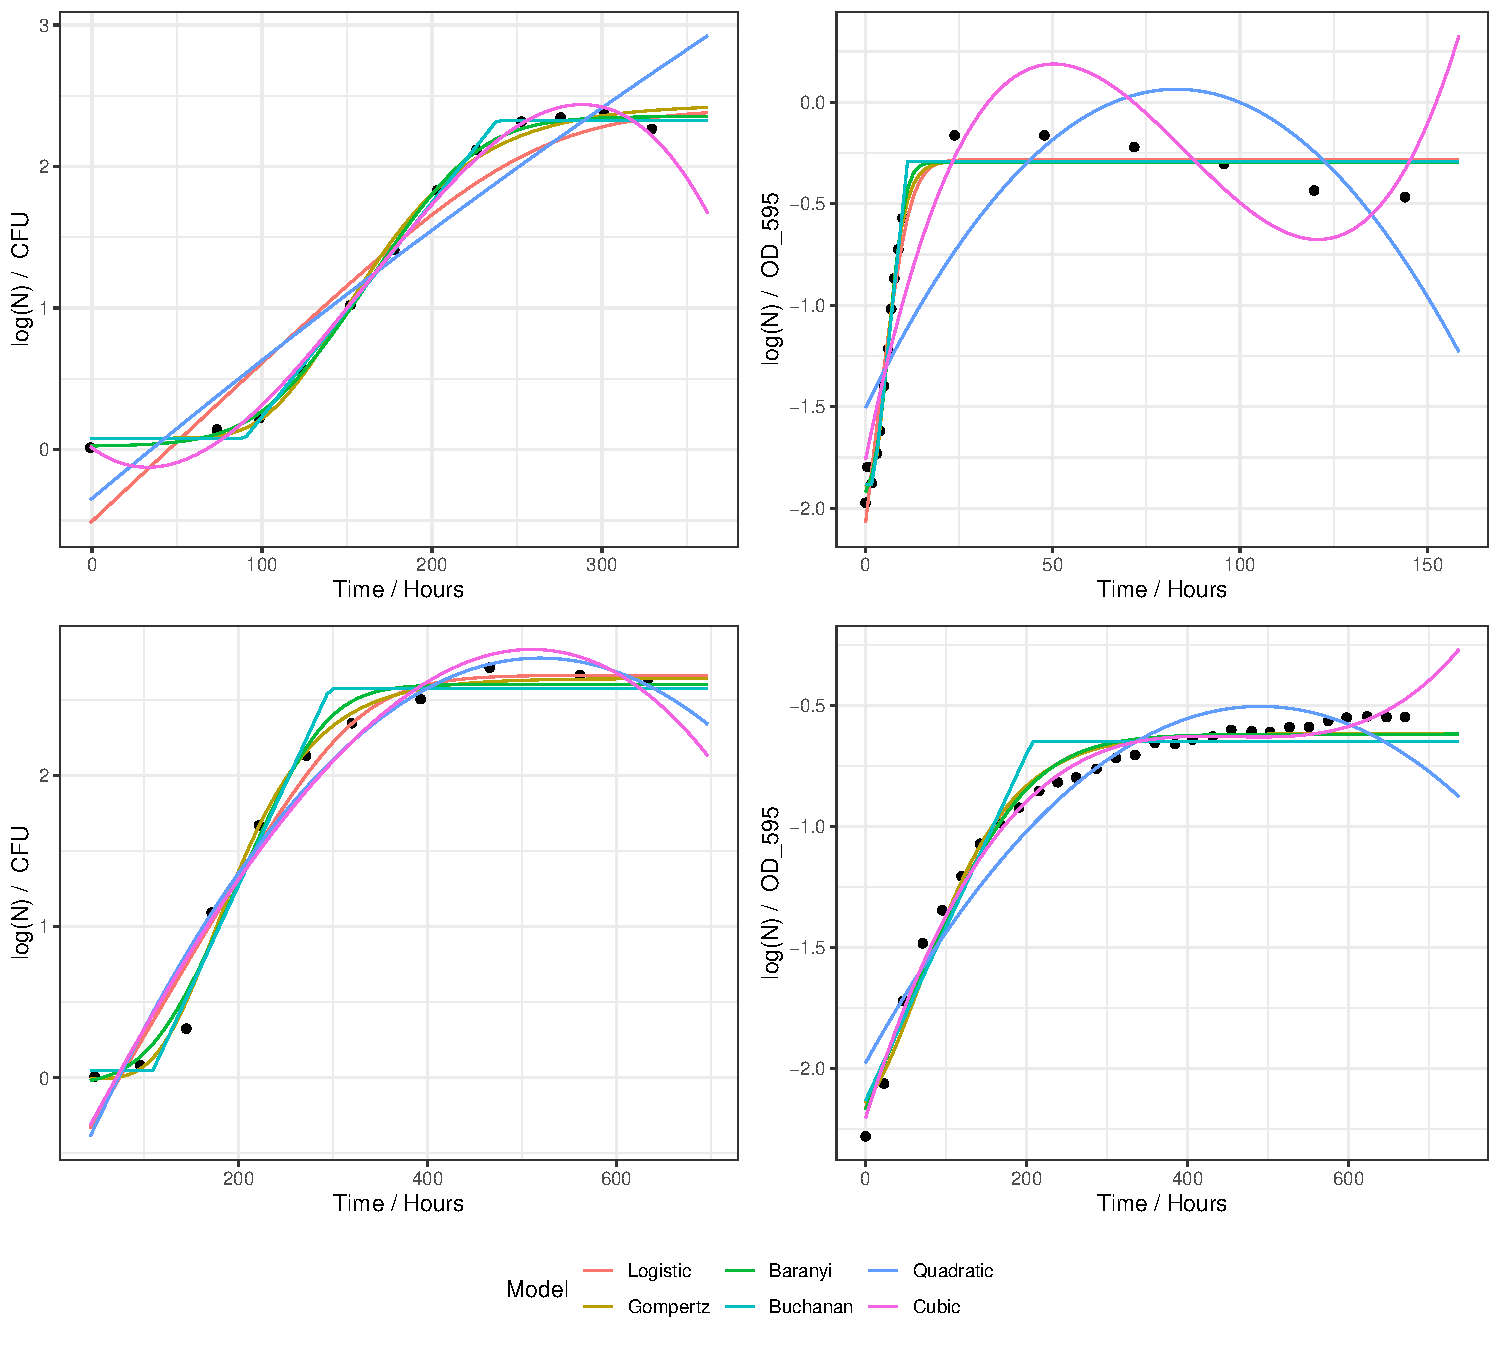
\includegraphics[height=4.5in]{../results/model_fits_linear.pdf}
        \caption{Demonstration of model fits in linear space. Out of 287 data sets, all fits were successful apart from a single fit of the Buchanan model, to a dataset which was removed anyway.}
        \label{sup:model_fits_linear}
        \end{figure}

         \begin{figure}[H]
        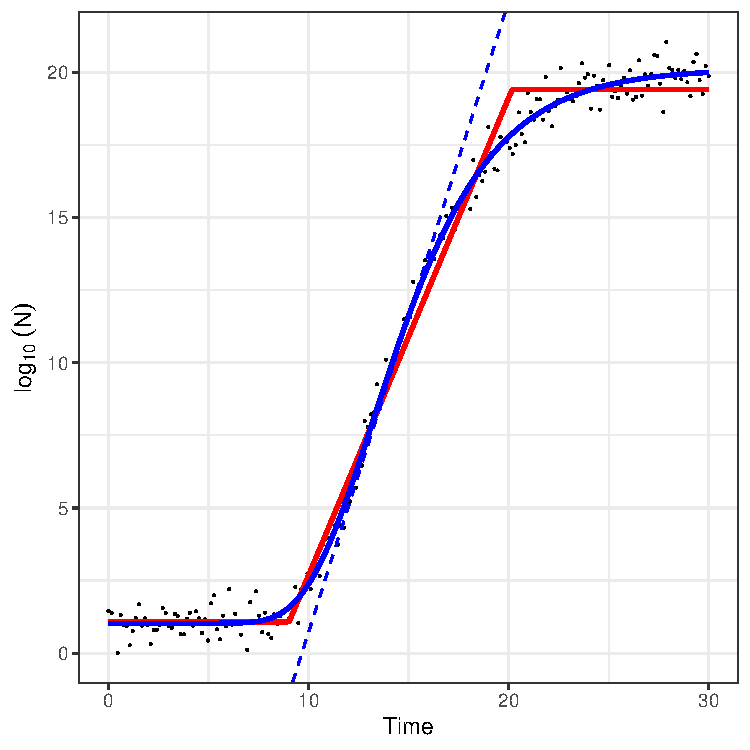
\includegraphics[width=4in]{../results/fit_difference.pdf}
        \centering
        \caption{The Buchanan and Gompertz models are fit to the same hypothetical growth data, which results in smaller $t_{lag}$ and $\mu_{max}$ estimates from the Buchanan model in order to capture the start of the growth phase. By contrast, there is some growth before $t = t_{lag}$ in the Gompertz model.}
        \label{sup:fit_difference}
        \end{figure} 
        
        
         \begin{figure}[H]
        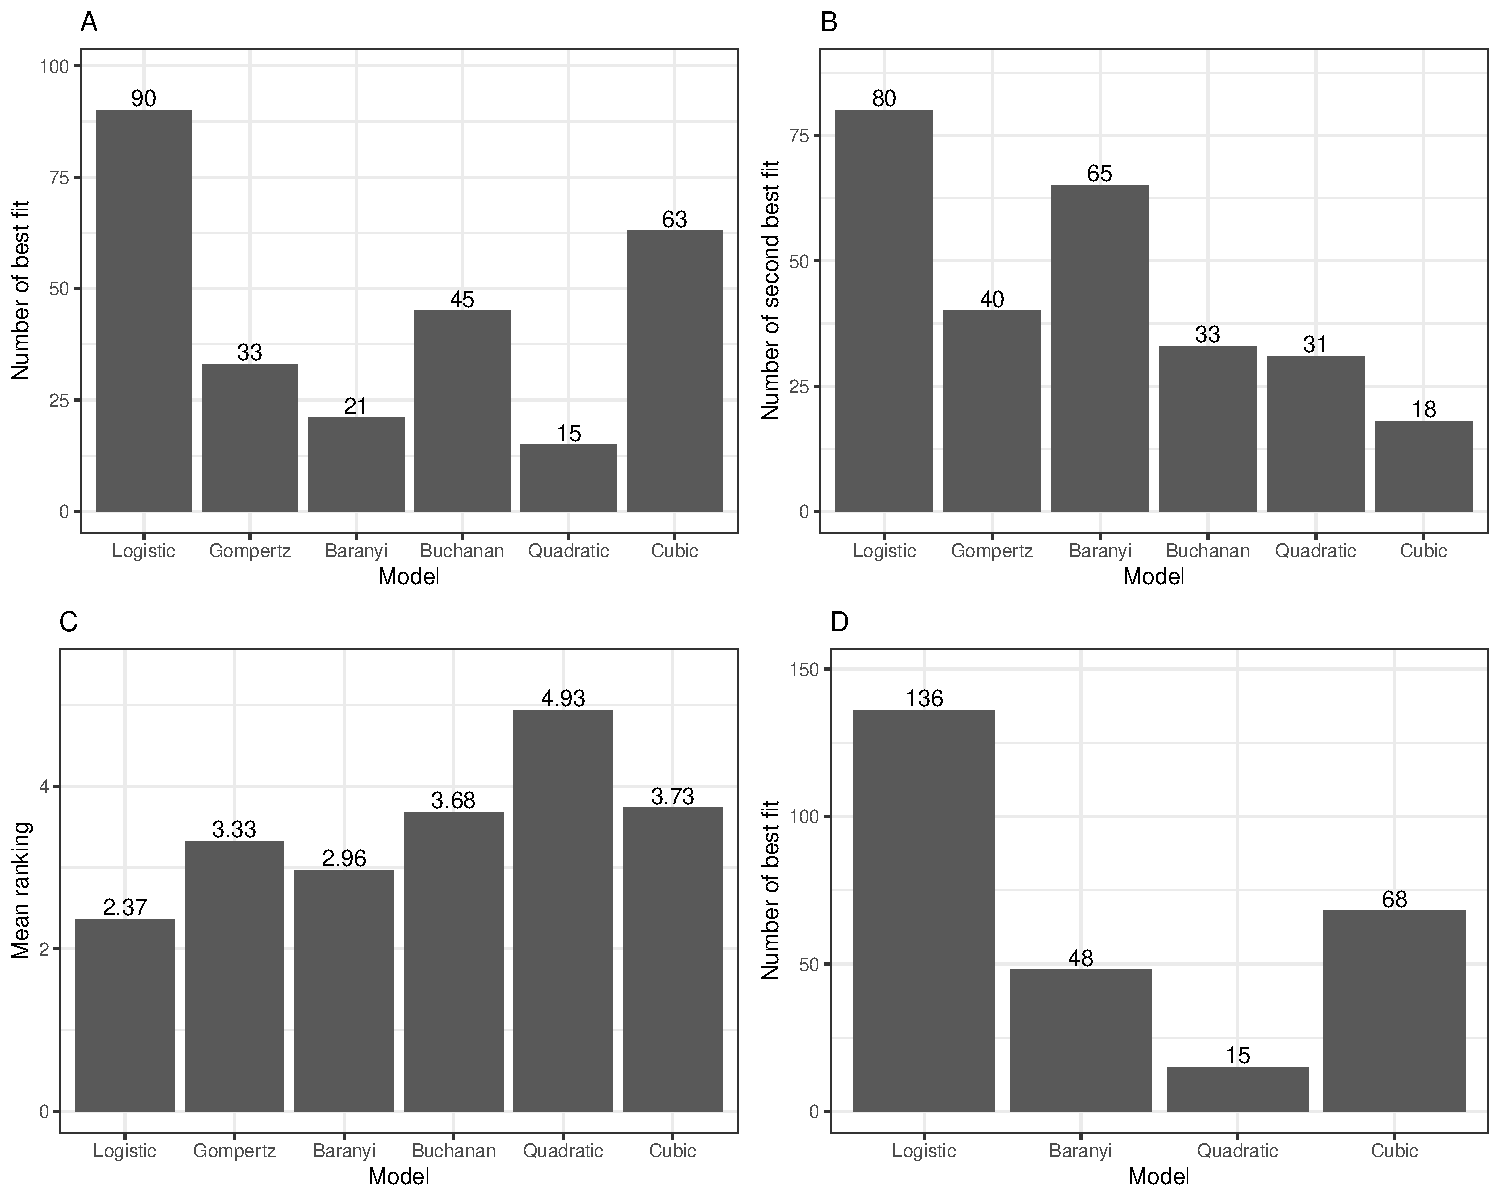
\includegraphics[width=4in]{../results/best_fit_frequency_bar_linear.pdf}
        \centering
        \caption{Plots showing rankings of models in linear space. (A) shows the number of times each model is the best fitting model for a dataset. (B) shows the number of times each model is the second best fitting model for a dataset. (C) shows the mean ranking for each model. (D) shows the number of times each model is the best fitting model for a dataset if we do not consider the Gompertz and Buchanan models.  In linear space, the logistic model performs better than it does in log space, as less emphasis is put on the lag phase.}
        \label{sup:frequency_bar_linear}
        \end{figure} 
        
\begin{table}[H]
\centering
\begin{tabular}{l|llllll}
       & Logistic & Gompertz & Baranyi & Buchanan & Quadratic & Cubic \\ \hline
AIC & 62.3    & 61.8    & 61.3   & 65.5    & 76.3     & 67.7 \\
BIC & 63.8    & 63.8    & 63.3   & 67.5    & 77.8     & 69.7 \\
$A_w$ & 0.213     & 0.174    & 0.158   & 0.178     & 0.0493     &   0.229

\end{tabular}
\caption{Mean AIC, BIC, and Akaike weight values for each model fitted in linear space}
\label{suptable:meanAICBIClinear}
\end{table}




        
        \begin{figure}[H]
        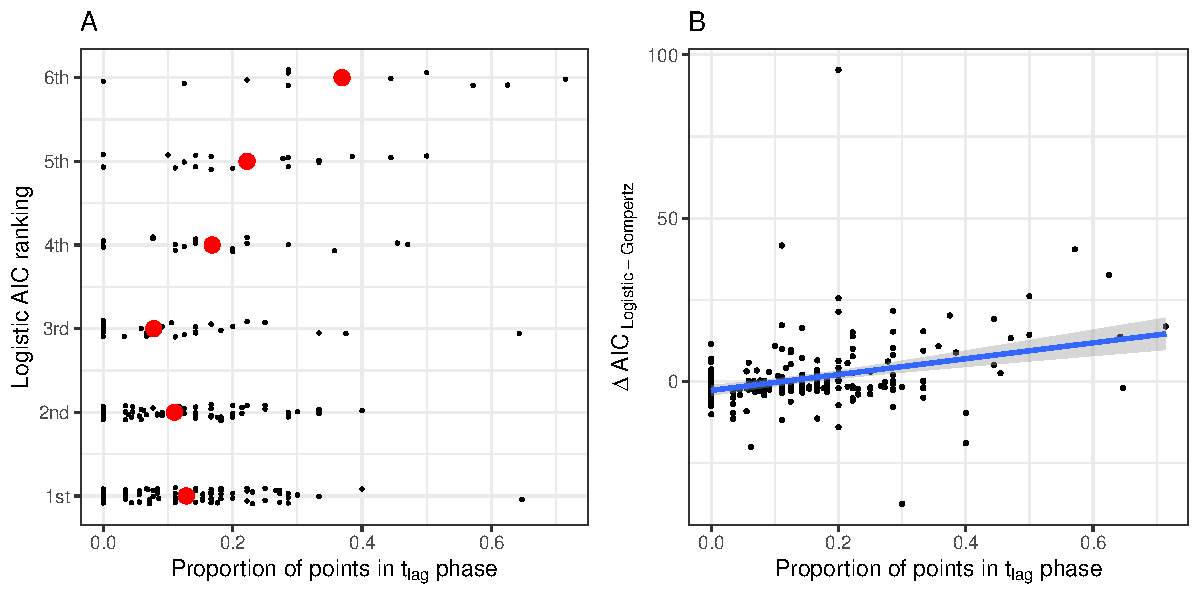
\includegraphics[width=5in]{../results/tlag_vs_logistic_linear.pdf}
        \centering
        \caption{(A) is a plot of proportion of points in the lag phase, against the ranking of the Logistic model by AIC in linear space. (B) shows the difference in AIC score between the Gompertz and Logistic model against this proportion, In both cases, the relationship between Logistic model performance and $t_{lag}$ is much weaker than in log space. The difference in AIC between Logistic and Gompertz decreases by 2.4 for every increase in lag phase proportion by 0.1 (in contrast to 6.9 for log space)}
        \label{sup:tlag_logistic_linear}
        \end{figure} 
        
         \begin{figure}[H]
        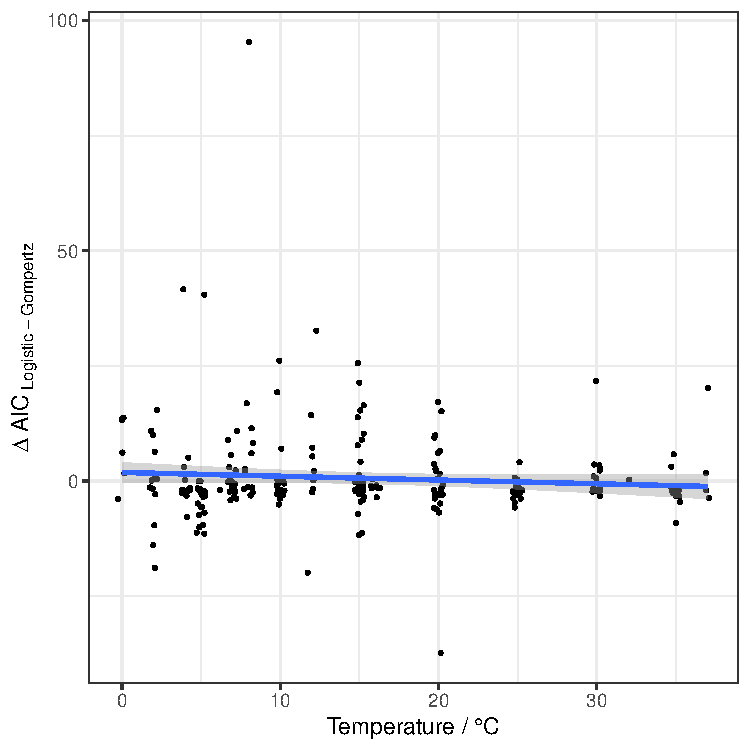
\includegraphics[width=3in]{../results/logistic_vs_gompertz_temp_linear.pdf}
        \centering
        \caption{$\Delta_{\text{Logistic - Gompertz}}$ no longer has a statistically significant relationship with temperature when models are fit in linear space. This implies that the fit of the Logistic model does not become any weaker realtive to thegompertz model as temperature increases.}
        \label{sup:logistic_temp_linear}
        \end{figure} 
        
        \begin{figure}[H]
        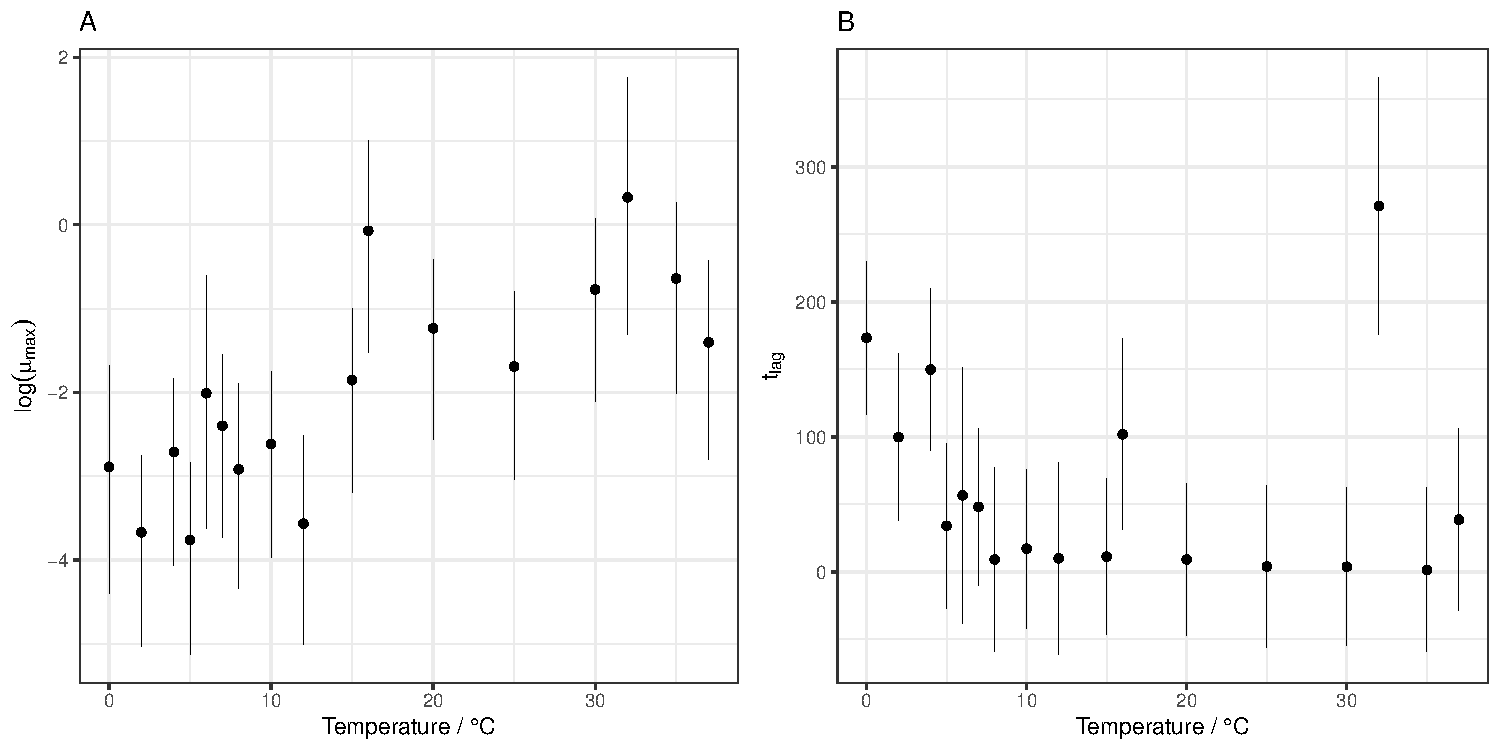
\includegraphics[width=\linewidth]{../results/tlags_linear.pdf}
        \centering
        \caption{The broad patterns of $\mu_{max}$ and $t_{lag}$ are the same when model fitting is in linear space, but the confidence intervals are much broader.}
        \label{sup:params_linear}
        \end{figure} 
        
        
    \bibliographystyle{ieeetr}
    \bibliography{write_up}

\end{document}
}

\newcommand{\beginsupplement}{%
        \setcounter{table}{0}
        \renewcommand{\thetable}{S\arabic{table}}%
        \setcounter{figure}{0}
        \renewcommand{\thefigure}{S\arabic{figure}}%
}


\setcounter{secnumdepth}{0}
\begin{document}

    \begin{titlepage}
	\centering
	
\includegraphics[width=0.5\textwidth]{../data/imperial.png}\par\vspace{1cm}
	\vspace{2cm}
	{\scshape\Large\bfseries Recommendations for Fitting Microbial Growth Models\par}
	\vspace{2cm}
	{\Large Sam Turner\par}
	\vspace{0.5cm}
	{\Large March 2020 \par}
	\vspace{0.5cm}
	{\Large\itshape Computational Method in Ecology and Evolution MSc\par}
	\vspace{0.5cm}
	 \wordcount words 
	\vfill

	\vfill
    
    \newpage
    \end{titlepage}
    

    \begin{abstract}
   Modelling of microbial growth is vital for developing food preservation measures to decrease food waste. By fitting a range of mechanistic and phenomenological models to a large dataset of 305 growth curves, I demonstrate that temperature has a major impact on microbial population dynamics. I also examine how methodological choices can influence the results of model fitting studies, including demonstrating that the choice of model can systematically bias parameter estimates to the extent that they become incomparable for meta-analysis. Improvements in the resolution of parameter estimates when models are fit in logarithmic space relative to linear space model fitting are also reported. These findings result in recommendations for microbial modelling methodology, particularly when data are aggregated across sources.
\end{abstract}
\tableofcontents
\begin{linenumbers}
    \section{Introduction}
    
    There is great interest in modelling the growth of microbial populations, in order to understand their response to external variables \cite{zwitmodelling}. This allows prediction of shelf lifes and optimisation of preservation methods. In this project, I address four questions:    

\begin{enumerate}
  \item Which models best describe microbial population growth, and how does this vary with temperature?
  \item How does temperature affect microbial growth?
  \item How does choice of model affects parameter estimates?
  \item Does the choice to fit models in linear or logarithmic space affect results?
  \end{enumerate}


I addressed these by fitting mechanistic and phenomenological models to a dataset of 305 digitised growth curves. Each mechanistic models describes the growth curve with a mathematical relationship representing a hypothesis about the dynamics of microbial growth \cite{Buchanan}, so is parameterised with meaningful biological quantities. In contrast, the phenomenological models are simply convenient mathematical functions used to describe patterns in the data, and are used as a neutral comparison for the mechanistic models. By comparing the fit of the mechanistic models to each other, and to the phenomenological models, support for the underlying biological hypothesis can be determined. I also examine the effect of temperature, both on the relative support for the models, and on the growth rate and lag time of microbial populations, as these play a central role in food spoilage. 

By comparing parameter estimates between models, and comparing results from fits in logarithmic and linear space, I also investigate how methodological choices can impact results. In particular, I was interested in whether differences in methodology could invalidate comparison of parameter values from different sources in meta-analyses.

\subsection{The Mechanistic Models}

The mechanistic models can be split into three four-parameter models, and the three-parameter logistic model. The four-parameter models split the growth curve into a lag phase, exponential phase, and stationary phase, with the logistic model discarding the lag phase.

\paragraph{Logistic}
The logistic model \cite{logisticVel1, logisticVel2} assumes that the microbial population immediately starts growing exponentially, with its growth rate falling towards zero as population size approaches a carrying capacity. This is described by the logistic differential equation:

\[ \frac{\mathrm d N}{\mathrm d t} =  \mu_{max}N(1-N)  \]

With solutions:

\[ N_t =   \frac{N_0  N_{max} e^{\mu t}}{N_{max} + N_0 (e^{\mu t} - 1)} \]


\subsubsection{Four-parameter models}

These models parameterise the sigmoidal growth curve with minimum and maximum population sizes, maximum growth rate, and a time lag before the population starts growing (illustrated in Figure \ref{fig:4_param_demo}). As such, the rate of growth and length of the lag phase can be independently varied (Figure \ref{fig:parameter_variation_demo})

        \begin{figure}[H]
        \centering
        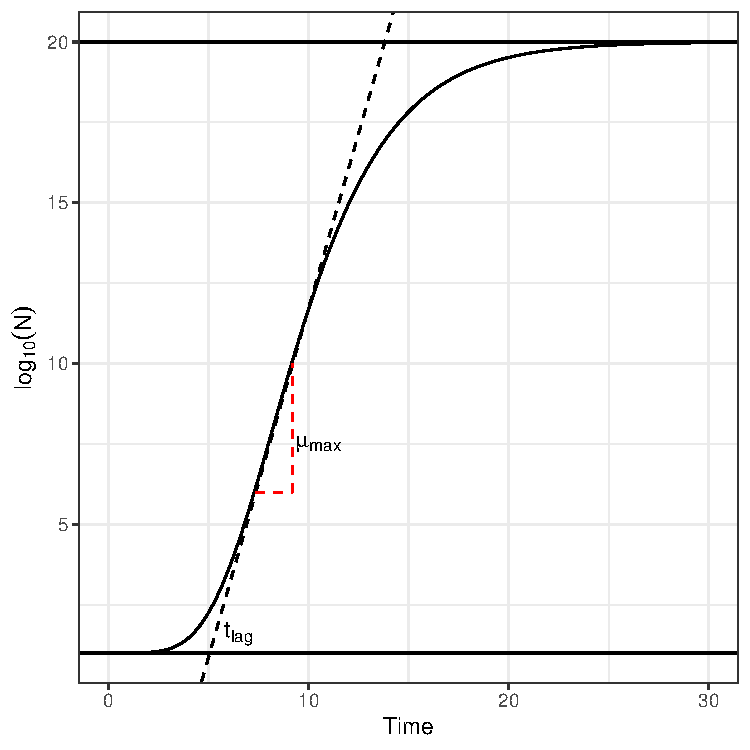
\includegraphics[width=4in]{../results/4_param_demo.pdf}
        \caption{Illustation of $\mu_{max}$ and $t_{lag}$ parameters. $\mu_{max}$ is the maximum gradient of the growth curve, and $t_{lag}$ is the intercept between this tangent line and the line $N = N_0$}
        \label{fig:4_param_demo}
        \end{figure}


        \begin{figure}[H]
        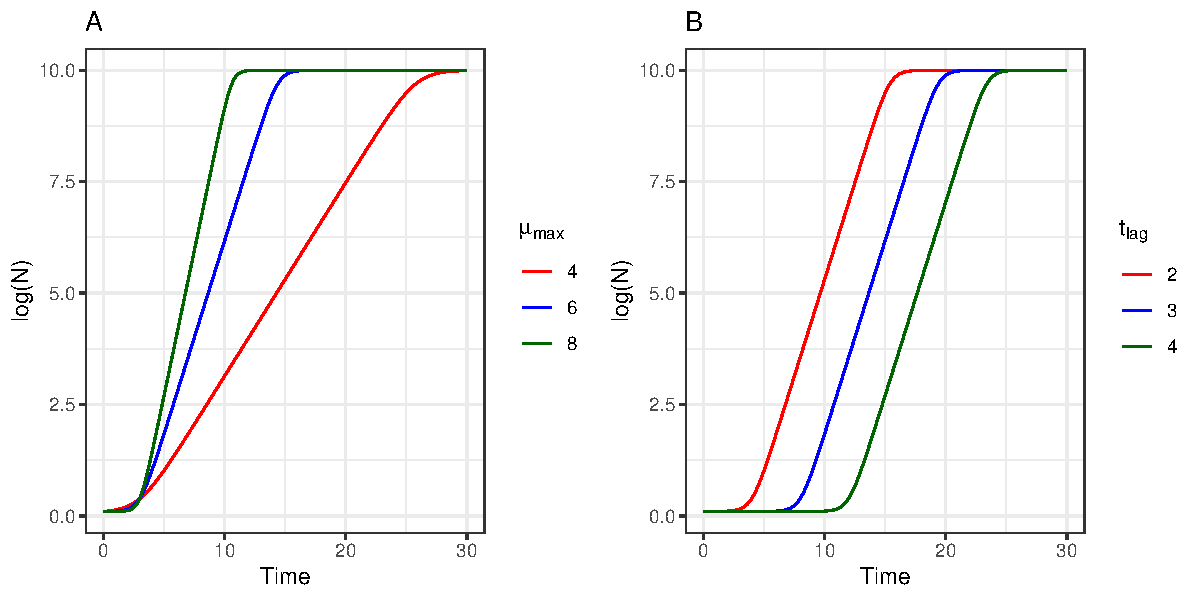
\includegraphics[width=\linewidth]{../results/tlag_rmax_demo.pdf}
        \caption{ $(A)\mu_{max}$ and (B) $t_{lag}$ parameters can be varied independently to control the rate of microbial growth, and the duration of the lag phase.}
        \label{fig:parameter_variation_demo}
        \end{figure}



\paragraph{Buchanan}
The Buchanan model \cite{Buchanan} is the simplest implementation of this, with a growth rate of zero during the lag and stationary phases, which surround a period of exponential growth:

  \[
    log(N_t) = \begin{cases}{}
        N_0 & \quad \text{if } t\leq t_{lag}\\
        N_0 + \mu_{max} \cdot (t - t_{lag}) &  \quad \text{if } t_{lag}\leq t\leq t_{max}\\
        N_{max} &  \quad \text{if } t\geq t_{max}
        \end{cases}
  \]

\paragraph{Gompertz}

The Gompertz model \cite{Gomp, zwitmodelling} describes a sigmoidal growth curve with a gradual transition into and out of the exponential phase. The Gompertz model has been popular for microbial population modelling, as it has empirically been found to fit well in a wide range of circumstances \cite{MicrobialGrowth}. However, it should be noted that its derivation does not have a mechanistic basis in microbial growth modelling \cite{EstBaranyi}, but rather in describing human mortality rates \cite{Gomp}. 

  \[log_{10}(N_t) = N_0 + (N_{max} - N_0)  e^{-e^{ \frac{\mu_{max} ~ \cdot ~ e  ~ \cdot ~ (t_{lag} - t)}{ (N_{max} - N_0) ~ \cdot ~ log(10)} + 1} }\]
  
  
\paragraph{Baranyi}

The Baranyi model is an attempt to formulate a truly mechanistic model for microbial population growth \cite{BaranyiOriginal, zwitmodelling}, explicitly modelling the internal physiological state and external environmental conditions of the cell. This produces a more flexible model, which can be applied to model population growth curves in time-varying environmental conditions. Here,  we use a version of the model in which conditions are homogenous, with the curvature parameter into the exponential phase $\nu$ set to $\mu_{max}$, and curvature parameter out of the exponential phase $m$ set at an empirical estimate of 1:

\[ log_{10}(N_t) = N_{max} + log_{10}(\frac{-1 + e^{\mu_{max} \cdot  t} + e^{\mu_{max} \cdot t_{lag}  } }{ -1 + e^{\mu_{max} \cdot t}  + e^{\mu_{max} \cdot t_{lag}} \cdot 10^{N_{max}-N_0}}) \]


        \begin{figure}[h]
        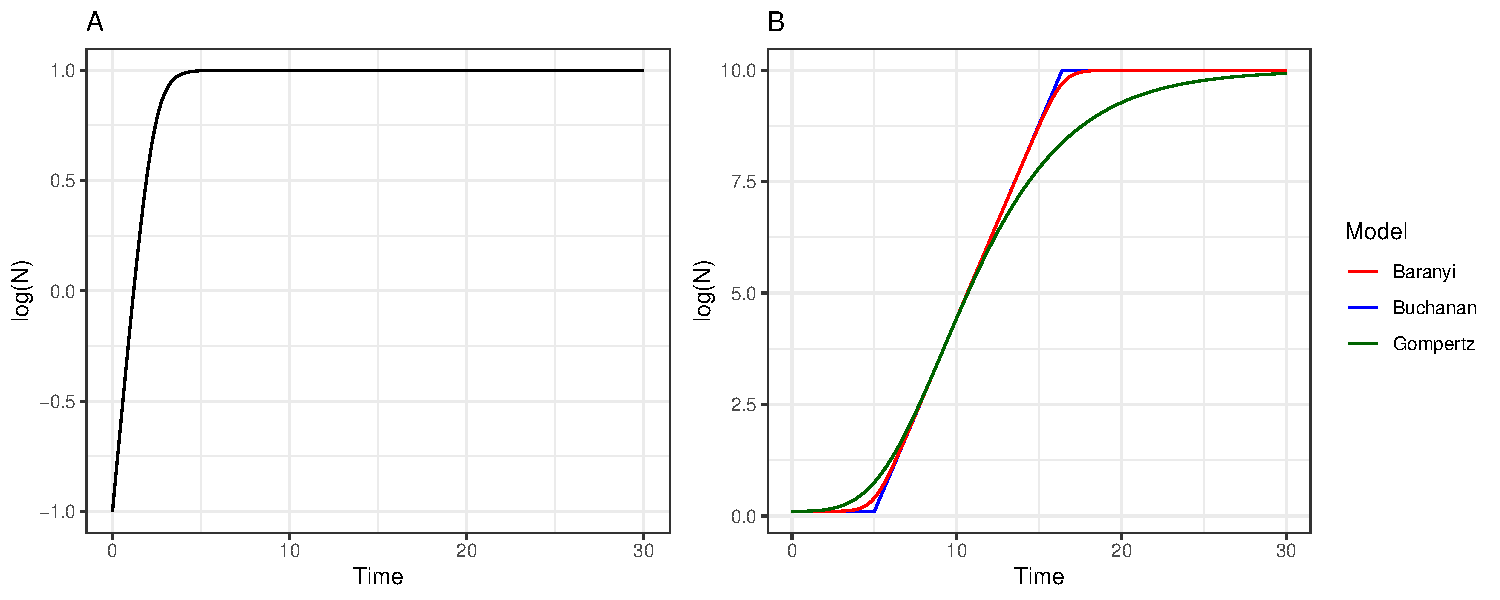
\includegraphics[width=\linewidth]{../results/model_demo.pdf}
        \captionsetup{format=hang}
        \caption{Demonstration of the shape of the 4 mechanistic models, plotted in log space. The logistic model (A) immediately starts growing at its maximum growth rate, whilst the three four-parameter models (B) have growth phases that transition into the exponential phase}
        \label{fig:models_demo}
        \end{figure}

\subsection{Phenomenological models}
As controls, I decided to fit quadratic and cubic polynomials to the data:
\paragraph*{Quadratic} $ N_t = at^2 + bt + c $
\paragraph{Cubic} \quad \quad $ N_t = at^3 + bt^2 + ct + d $


   \section{Methods}
   
   \subsection{Data}
   
\paragraph{Data sources}
The provided microbial growth data contained 305 time series, digitised from graphs in 10 papers from the microbial growth literature. The data set contained time series from 47 different species, 18 media, and 17 temperatures, with population size measured in 4 different units. However, the data from one citation \cite{discarded} clearly had incorrect time values, with times extending to 13,000 hours. I removed the data from this citation as there was not a clear correct transformation to produce the correct times, leaving 287 time series for analysis.

\paragraph{Log transformation}
As explained below, I decided to fit the model to $log_{10}(N)$ as well as to linear data. In 5/287 data sets, there were negative population counts due to numerical error in growth curve digitization. One value of approximately -668 was removed, whilst other negative values were greater that -10\textsuperscript{-2}; in these cases, I transformed increased population sizes for that time series by the minimum population size in the time series, discarding the minimum value of 0 before taking the logarithm.  

\paragraph{Time transformation}
I transformed each time series to start at $t = 0$ when fitting the four-parameter models, as model fits were clearly suboptimal without this transformation. Since $t_{lag}$ directly transforms the curve along the t-axis, $t_{lag}$ could be adjusted back to obtain model parameters which fit the untransformed time series. 

\subsection{Model Fitting}
When fitting the models, I used a least squares approach, both to log\textsubscript{10} transformed data, and to the original linear data (Figure \ref{sup:compare_least_squares}). This required exponentiating the four-parameter models to predict linear population size, and taking the logarithm of the logistic model to predict logarithmic population size. As such, the parameters of the four-parameter models remained in logarithmic space, and the parameters of the Logistic model in linear space. 

Due to the advantages presented in Results, I analysed parameter estimates from the log-fitted models (although linear fit results are presented in the Supplementary Figures), also choosing not to linearise residuals as this resulted in non-sensical fits (demonstrated in Figure \ref{sup:compare_least_squares}). These fits can be explained by the fact that, in general:
\[log(f(x) ) \neq f(log(x))\]
This means minimising errors in logarithmic space does not result in minimised errors in linear space, so evaluating fit in linear space does not capture the best possible fit for each model, (Figure \ref{sup:compare_least_squares}).

\subsubsection{Fitting linear models}

The two polynomial phenomenological models are linear in their parameters, so were fitted using Ordinary Least Squares with the lm() function in R \cite{R}.

\subsubsection{Fitting non-linear models}

The mechanistic models are non-linear, so are fitted using an optimisation approach. The nlsLM function in the minpack.lm \cite{minpack} package uses the Levenberg-Marquardt algorithm to optimise initial values to determine best fitting parameter values for a specified model. If initial values are far from the optimal parameters, it is likely that the optimisation will not converge, or will converge to very suboptimal parameters. It is therefore important to estimate reasonable starting values.

\paragraph{Estimating parameter values}
N\textsubscript{min} and N\textsubscript{max} were set as the minimum and maximum observed population size respectively. $\mu_{max}$ and $t_{lag}$ estimates were determined using a rolling regression (Figure \ref{sup:rolling_regression}), which computed the regression line for all sets of 5 adjacent data points. The regression line with the greatest gradient was selected, with the gradient taken as an estimate of $\mu_{max}$, and the $t$ value at the intercept between this regression line and $N = \min(N)$ taken as the $t_{lag}$ estimate. This was repeated in both logarithmic and linear space to provide parameter values for Logistic and four-parameter models.


\paragraph{Multiple fit attempts}
Despite well chosen initial values, models often fail to converge, or converge to poorly fitting parameter values. To increase the proportion of models which fit, and ensure that I find parameter values nearer the global optimum, I used a grid search to explore a range of initial parameter values. For each parameter, I chose linearly spaced samples from a range surrounding the estimate of that parameter value, and fitted a model for every combination of these parameter values. For example, if I take 3 samples for each of $N_0$ and $N_{max}$, and 5 for $t_{lag}$ and $\mu_{max}$, I fit $3 \times 3 \times 5 \times 5 = 225$ models. From the model fits that converge, I select the model with the smallest RSS. If none converge, I randomly sample parameter values with normally distributed noise around my parameter estimates until a model fits, or until there have been 1,000 failed attempts. 

Using this method, I was able to fit all 287 data sets for the Logistic, Gompertz, and Baranyi models in both linear space and logarithmic space. In linear space, there was one failed fit for the Buchanan model, and in log space there were two failed fits for the Buchanan model.


\subsection{Filtering}
Some data sets show no pattern of population growth, or have too few points in the growth phase to constrain the $mu_{max}$ and $t_{lag}$ parameters. I visualised the 64 data sets with the lowest maximum R\textsuperscript{2} value, removing 20 with no meaningful growth pattern or visibly little constraint (Figure \ref{sup:removed_ids}). For parameter estimate analysis, I further filtered out datasets with fewer than 2 points in the growth phase (Figure \ref{sup:constraint}) by counting the number of points with a time value within the predicted exponential phase, as determined using Akaike weighted parameter values. This removed a further 57 data sets, leaving 210 data sets.


\subsection{Model Selection}

Model fit was assessed using AIC \cite{AIC} and BIC \cite{BIC}. With the assumption of normally distributed errors, and simplification to remove constants, these are:
\[\text {AIC}  = 2k + n\log(RSS)\]
\[\text {BIC} = n\log{\frac{RSS}{n}} + k\log{n}\]


Both AIC and BIC balance fit against model complexity, allowing direct comparison of fit for models with differing numbers of parameters. However, BIC has the disadvantage of making a number of unrealistic assumptions about the true model: that it exists, is in the model set, and has equal prior probability to other models. Additionally, the fact that AIC is based in Kullback–Leibler information theory means that standardised model likelihoods - Akaike weights - can be calculated to naturally compare model support and allow model averaging \cite{Omland, ModelSelection}.


\subsection{Parameter Estimation}

Parameter estimation was performed using Akaike weights, which produce a single parameter estimate from a family of models \cite{ModelSelection}, weighted by the model’s relative likelihood.
With $\text{AIC}_{best}$ being the lowest observed AIC values for a dataset, $\Delta_{AIC}$ values are calculated with:
\[ \Delta_i = \text{AIC}_i - \text{AIC}_{best} \]

The Akaike weight for the $i^{th}$ model is then:
\[ w_i = \frac{e^{-\frac{1}{2}\Delta_i }} { \sum_{r = 1}^{r = R}  e^{- \frac{1}{2}\Delta_r }}\]

The Akaike weighted parameter estimate for $\theta$, with weights $w_i$ and individual model parameter estimates $\theta_i$ is:
\[\theta_w = \sum_{i = 1}^{i = I}\theta_i * w_i\]


\subsection{Statistical Analysis}

I ran linear regressions of $\Delta_{\text{Logistic - Gompertz}}$ against temperature, and $\Delta_{\text{Logistic - Gompertz}}$ against proportion of points in the lag phase, using lm() in R \cite{R}. Their diagnostic plots were examined to confirm the suitability of a linear model.

I ran a mixed effects model of $\mu{max}$ against temperature, and of $t_{lag}$ against temperature, with species and medium used as random effects in each case. Again, diagnostic plots were used to confirm that residuals were homogeneous across the fitted values.

I ran a paired t-tests for $\mu_{lag}$ and $t_{lag}$ between the each pair of four-parameter models, and between linear and logarithmic space fits, to check for systematic differences in parameter estimates. I check for normality of differences by plotting histograms of these differences.  

\subsection{Computing Tools}
\paragraph{R 3.6.1 \cite{R}} was used for initial data preparation script, model fitting, analysis, and figure preparation. R was chosen because the native data structures are naturally suited to this type of data, and support of vectorised operations makes the code cleaner than it would be in Python. I used R for my multi-start method to fit models over a range of initial parameter values because of the efficiency of non-linear least squares model fitting in the minpack.lm package. \textbf{minpack.lm \cite{minpack}} was used for non-linear least squares model fitting using the more robust Levenberg-Marquardt algorithm (relative to Gauss-Newton). \textbf{ggplot2 \cite{gg}} was used to create high quality graphics. \textbf{dplyr \cite{dplyr}} was used for data wrangling. \textbf{lme4 \cite{lme4}} was used to fit linear mixed models. \textbf{toOrdinal \cite{tO}} was used for annotations.

\paragraph{Python 3.7.4 \cite{python}} was used for calculation of initial values. \textbf{pandas \cite{pd}} was used for dataframes in Python. \textbf{matplotlib \cite{plt}} was used to create graphics in Python. \textbf{SciPy \cite{numpy}} was used to fit linear regressions for the rolling regression. \textbf{NumPy \cite{numpy}} was used for efficient arrays.

\paragraph{bash 3.2} was used to write scripts tying other elements of the project together.

\paragraph{\LaTeX } was used for compilation of this write-up.
\section{Results}

\subsection{Model fitting is highly successful}
Taking the best fitting model from a range of initial parameter values was very effective, with all models converging to every data set when those with no discernible growth pattern were removed, and only 3 unsuccessful fits otherwise (2293 / 2296 successful non-linear fits overall). Model fits were visually inspected, and found to describe the data well (Figure \ref{fig:model_fits} for logarithmic fits, Figure \ref{sup:model_fits_linear} for linear fits). For the reasons expanded on in the Discussion, I present the results obtained from fitting models in logarithmic space first, before examining the results from linear space fits at the end of this section.

         \begin{figure}[H]
         \centering
       	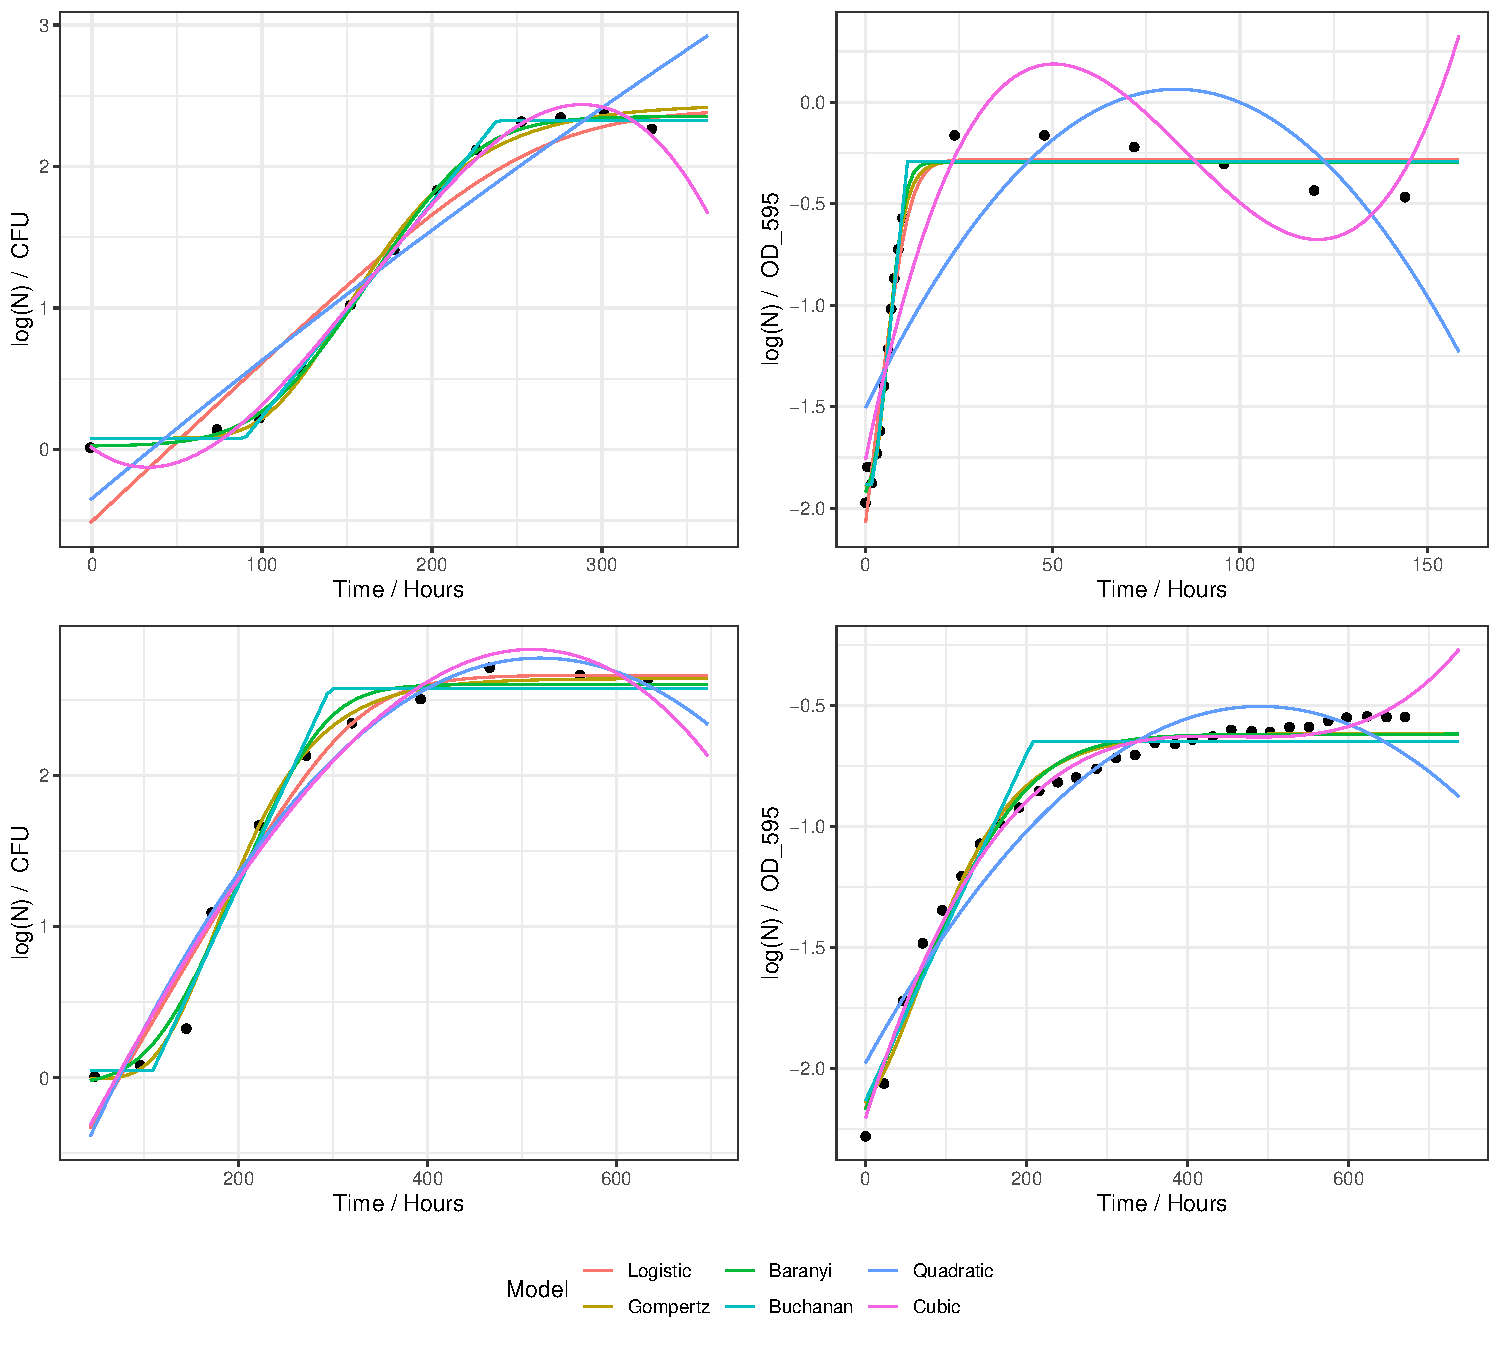
\includegraphics[height=4.5in]{../results/model_fits.pdf}
        \caption{Demonstration of model fits in log space. Out of 287 data sets, all fits were successful apart from two fits of the Buchanan model, to datasets which were removed anyway. }
        \label{fig:model_fits}
        \end{figure}

\subsection{Gompertz and Baranyi are best supported}

The Gompertz model and Baranyi model are both well supported by the data. The Gompertz model most frequently has the lowest AIC (Figure \ref{fig:bestbars} A), and has the highest mean Akaike weight (Figure \ref{AWdist} and Table \ref{tab:meanAICBIC}). However, the Baranyi model has a lower mean ranking (Figure \ref{fig:bestbars} C), and lower mean AICs and BICs. (Table \ref{tab:meanAICBIC}). It appears that the Baranyi model is a consistent good fit to the data, achieving the lowest mean AIC despite relatively rarely being the best fitting model - as evidenced by it placing second for nearly half of the datasets (Figure \ref{fig:bestbars} B).



        \begin{figure}[H]
        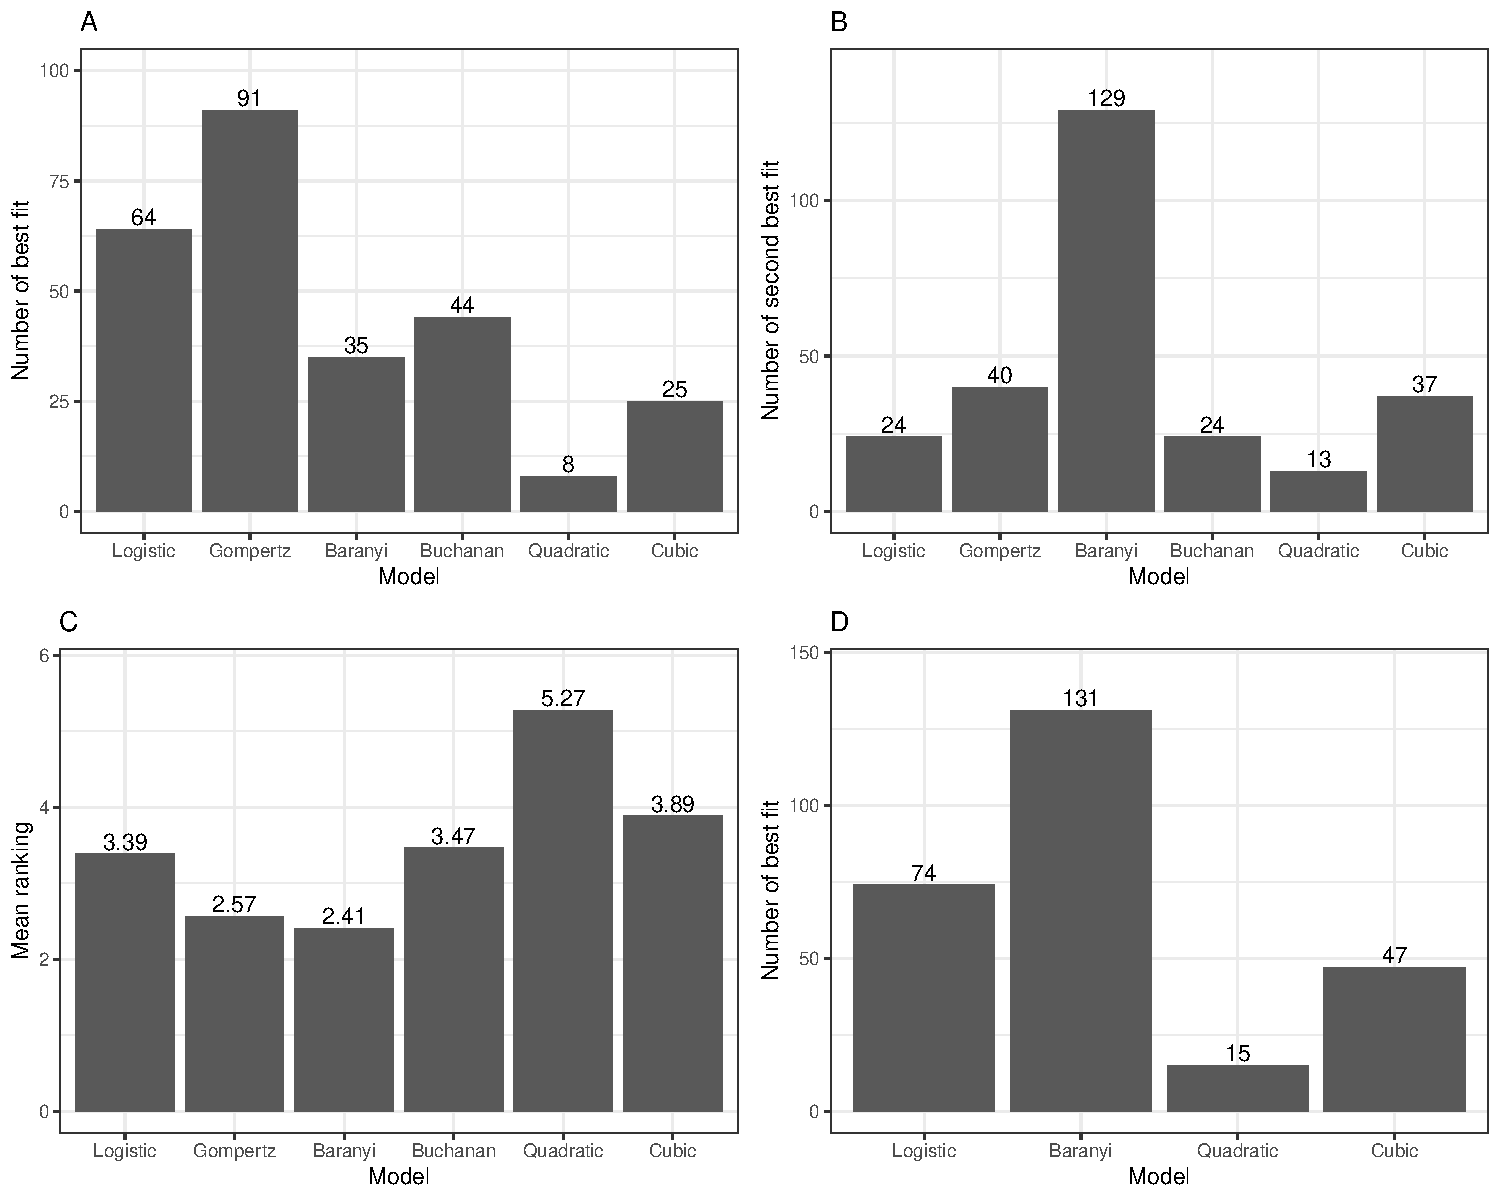
\includegraphics[width=\linewidth]{../results/best_fit_frequency_bar.pdf}
        \caption{Plots showing the rankings of models in logarithmic space. (A) shows the number of times each model is the best fitting model for a dataset. (B) shows the number of times each model is the second best fitting model for a dataset. (C) shows the mean ranking for each model. (D) shows the number of times each model is the best fitting model for a dataset if we do not consider the Gompertz and Buchanan models. }
        \label{fig:bestbars}
        \end{figure}
        
         \begin{table}[H]
	\centering
	\begin{tabular}{l|llllll}
       & Logistic & Gompertz & Baranyi & Buchanan & Quadratic & Cubic \\ \hline
AIC & -58.5    & -66.2    & -66.3   & -61.1    & -43.7     & -53.2 \\
BIC & -57.0    & -64.1    & -64.2   & -59.1    & -42.2     & -51.1 \\
$A_w$ & 0.162     & 0.316     & 0.218   & 0.156     & 0.0319     & 0.116
	\end{tabular}
	\caption{Mean AIC, BIC, and A\textsubscript{w}  values for each model, fitted in logarithmic space. Lower AIC represents greater relative support, whilst higher $A_w$ represents greater relative likelihood.}
	\label{tab:meanAICBIC}
	\end{table}




        \begin{figure}[H]
        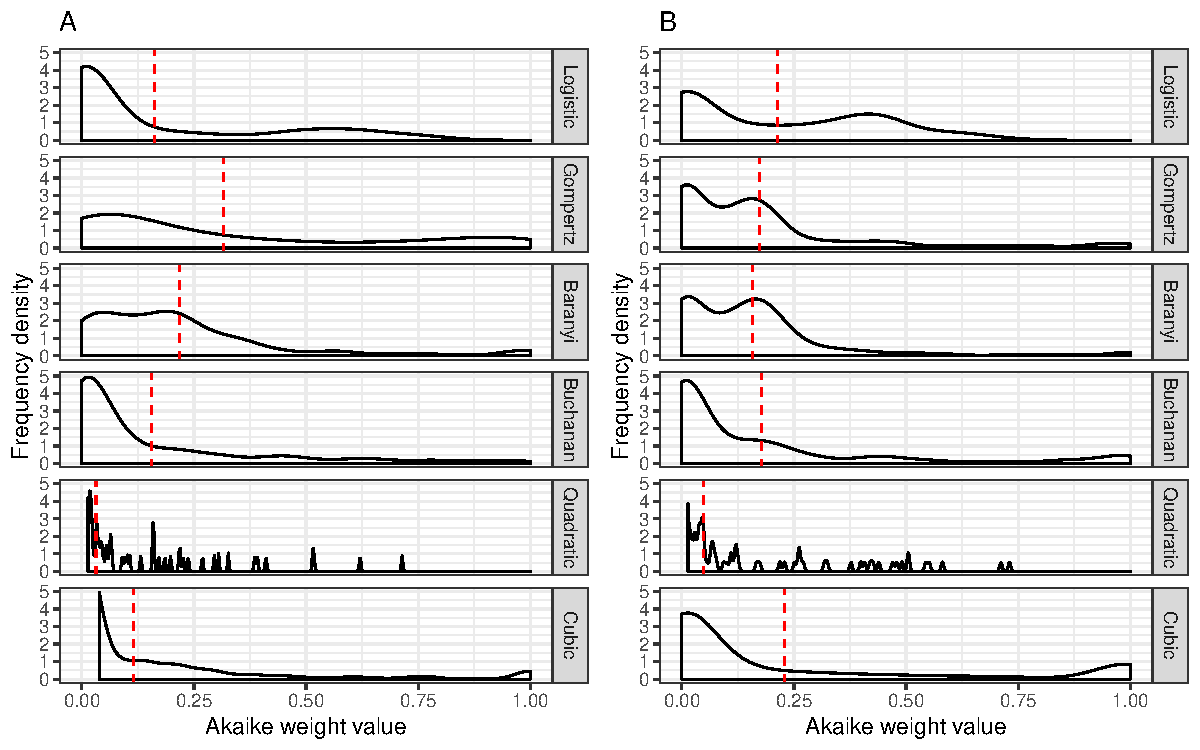
\includegraphics[height=3.5in]{../results/Aw_distributions.pdf}
        \caption{Gaussian Kernel Density Estimates for Akaike weights in logarithmic (A) and linear (B) space for each model. We see that in logarithmic space, the Gompertz model has strongest support, with the Logistic model have highly variable support due to its inability to model $t_{lag}$. In linear space, poor lag phase modelling is less strongly penalised, so the Logistic model gains the most support. }
        \label{fig:AWdist}
        \end{figure}
        
        

        
        \subsection{Logistic fit is poor when t\textsubscript{lag} is high}
                
        Notably, the Logistic model is the best model second most frequently despite its mean AIC and BIC scores placing fourth best - implying great variability in its performance. We can see this variability in its A\textsubscript{w} distribution, with high probability density near zero but a relative high density in the 0.5 to 0.75 interval (Figure \ref{AWdist}.  This can be explained by the absence of a lag phase in the model: the Logistic model fits poorly when a lag phase is present, but fits well when it is absent without incurring the AIC/BIC penalty for a fourth parameter. This is evident in the increasing proportion of points in the lag phase as the ranking of the logistic model gets worse (Figure \ref{fig:logistic_tlag} A). More explicitly, the difference in AIC between the Logistic and Gompertz model increases with proportion of data points in the lag phase (Figure \ref{fig:logistic_tlag} B). This relationship is strongly significant, with a linear regression estimating an increase in $\Delta_{\text{Logistic - Gompertz}}$ of 6.9 for every increase in lag phase proportion of 0.1, with a standard error of 0.47.
        
                \begin{figure}[H]
        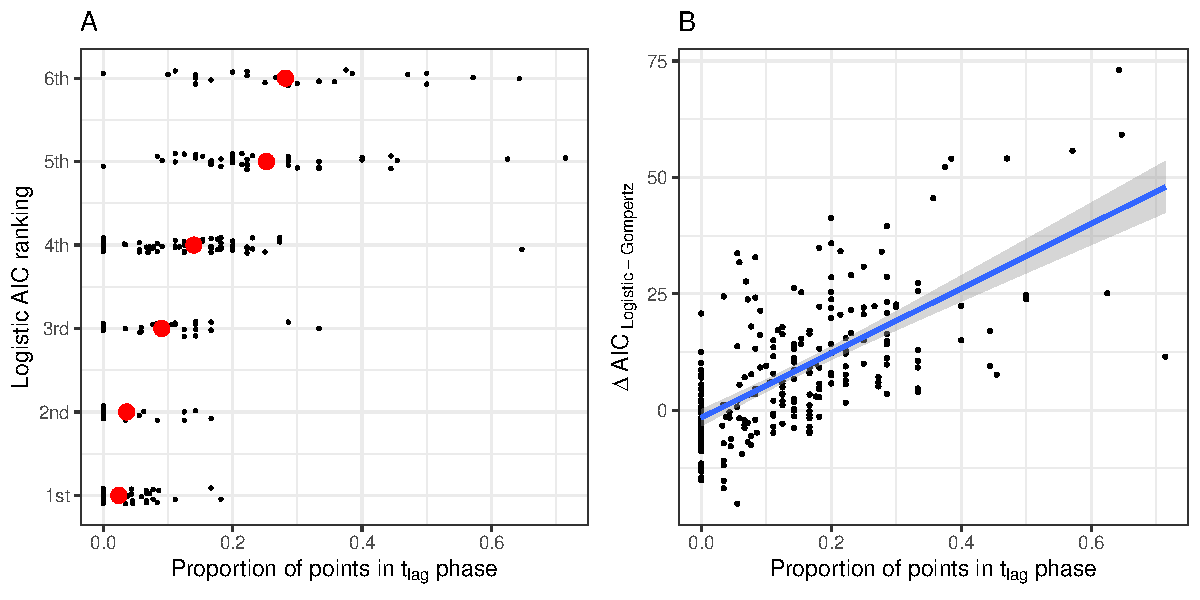
\includegraphics[width=\linewidth]{../results/tlag_vs_logistic.pdf}
        \caption{(A) is a plot of proportion of points in the lag phase, against the ranking of the Logistic model by AIC. We see that an increasing proportion of points in the lag phase is associated with a poorer ranking - with the mean proportion for each ranking shown by the red circle. (B) shows the difference in AIC score between the Gompertz and Logistic model against this proportion, with a statistically significant slope observed.}
        \label{fig:logistic_tlag}
        \end{figure}        
        
        \subsection{Temperature affects $\mu_{max}$ and $t_{lag}$}
        
         I ran a linear mixed model to determine the effect of temperature on $\mu_{max}$ and $t_{lag}$ across the entire data set, including species and medium as random effects. Temperature was included as a categorical variable as it is unlikely that the response to temperature is linear across the entire temperature range. From this, estimates for $\log(\mu_{max})$ and $t_{lag}$ values were be made for each temperature, shown in Figure \ref{fig:params_temp}. It is clear that the logarithm of the maximum rate of bacterial growth increases with temperature, approximately linearly across much of the temperature range, indicating an Arrhenius type thermal response. $t_{lag}$ decreases with temperature, quickly levelling off at around 10\degree C. 

         \begin{figure}[H]
        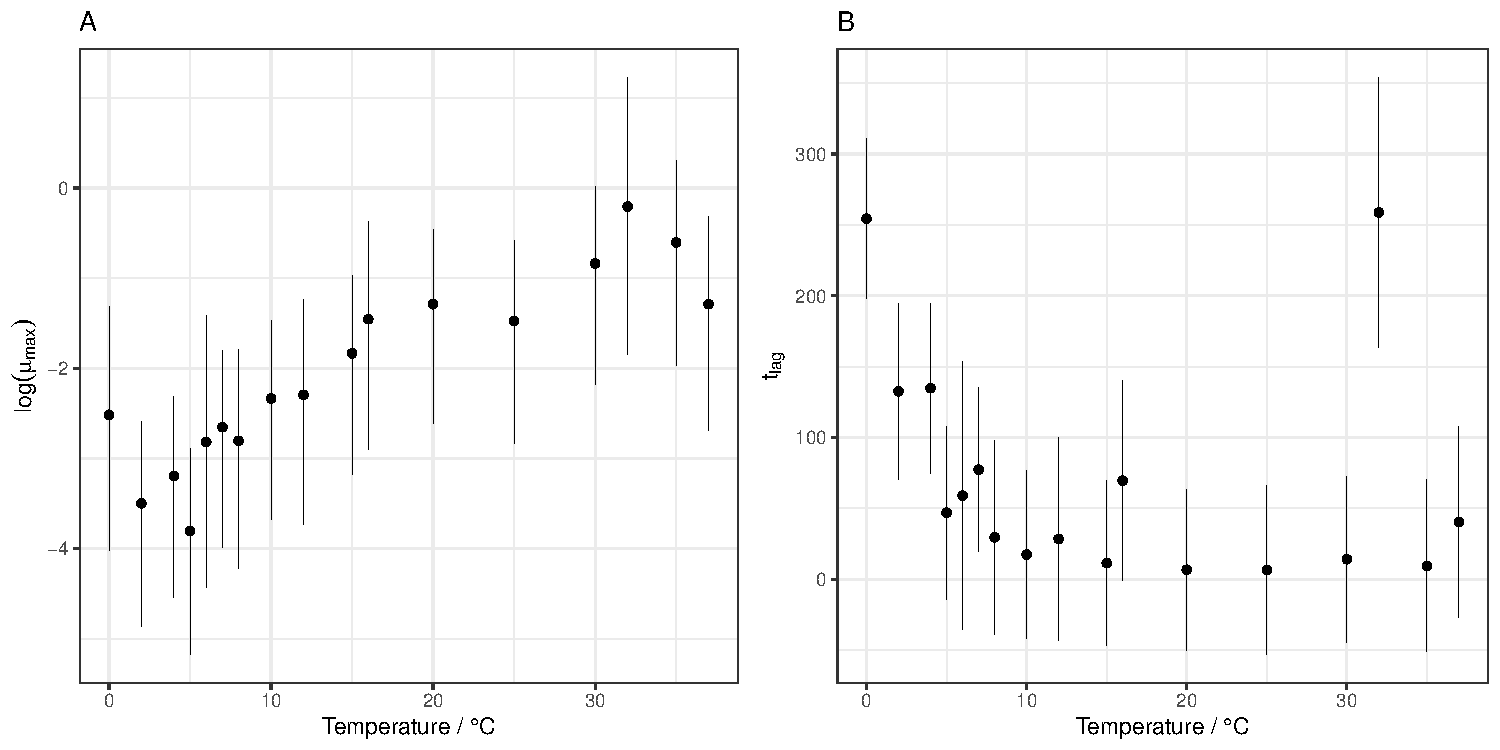
\includegraphics[width=\linewidth]{../results/tlags.pdf}
        \caption{(A) shows the relationship between $\mu_{max}$ and temperature, as estimated by a linear mixed model with temperature as a categorical variable. Vertical lines indicate the 95\% CI. $\mu_{max}$ increases steadily with temperature over the observed range. Similarly, (A) shows the relationship between $t_{lag}$ and temperature. We see that below 10\degree C, $t_{lag}$ increases rapidly as temperature decreases.   }
        \label{fig:params_temp}
        \end{figure}  



\subsection{Logistic model fits better at higher temperatures}

The decrease in $t_{lag}$ with temperature implies that the Logistic model, which has better fit with smaller $t_{lag}$, should have better fit with increasing temperature. Indeed, Figure \ref{fig:logistic_temp}A shows that $\Delta_{\text{Logistic - Gompertz}}$  decreases with increasing temperature. A linear regression suggests a decrease in $\Delta_{\text{Logistic - Gompertz}}$ of 3.30 for every 10\degree C, with standard error of 0.8.

        \begin{figure}[H]
        \centering
        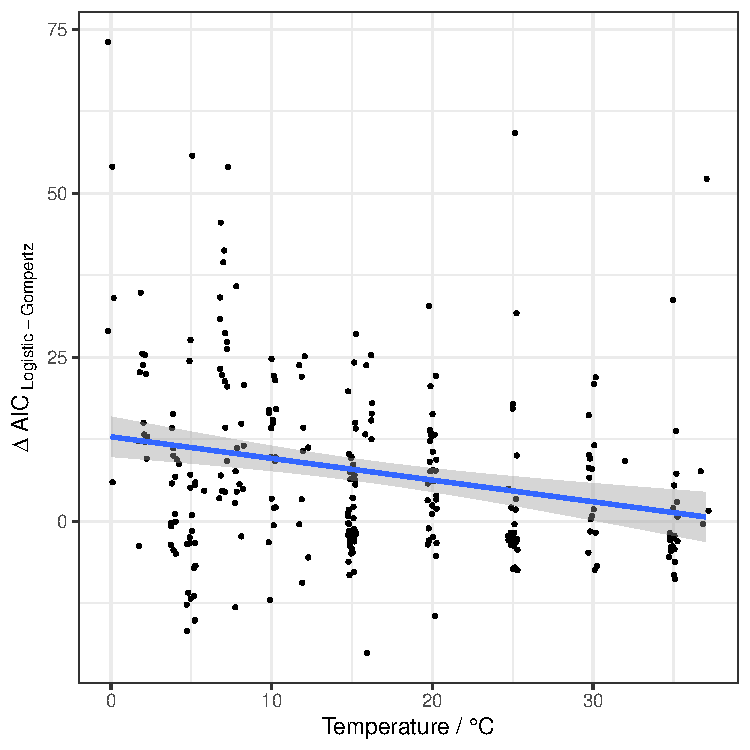
\includegraphics[width=4in]{../results/logistic_vs_gompertz_temp.pdf}
        \caption{$\Delta_{\text{Logistic - Gompertz}}$ is seen to decrease by 3.30 for every 10\degree C, indicating an improvement in the fit of the Logistic model relative to the Gompertz model as temperature increases.}
        \label{fig:logistic_temp}
        \end{figure}  

\subsection{Model choice biases parameter estimates}

Tables \ref{tab:tlag_biases} and \ref{tab:rmax_biases} show the mean pairwise differences in $t_{lag}$ and $\mu_{max}$ for the 4-parameter models. The Buchanan model results in the lowest $t_{lag}$ and lowest $\mu_{max}$ values. This is because the model assumes that population growth remains exactly at zero until $t = t_{lag}$, rather than smoothly transitioning to $\mu_{max}$ before this intercept. This means that Buchanan model fits must decrease $t_{lag}$ to capture the first part of the growth phase, consequently lowering $t_{lag}$ and $\mu_{max}$ values (Figure \ref{sup:fit_difference}).

\begin{table}[H]
\centering
\begin{tabular}{l|lll}
         & Gompertz                                        & Baranyi                                         & Buchanan                 \\ \hline
Gompertz & \cellcolor[HTML]{9B9B9B}                        & -5.21 = - 9.8\%                                           & 4.23 = 8.0\%                     \\
Baranyi  & \cellcolor[HTML]{9B9B9B}{\color[HTML]{9B9B9B} } & \cellcolor[HTML]{9B9B9B}{\color[HTML]{9B9B9B} } & 9.44 = 17.8\%                     \\
Buchanan & \cellcolor[HTML]{9B9B9B}{\color[HTML]{9B9B9B} } & \cellcolor[HTML]{9B9B9B}                        & \cellcolor[HTML]{9B9B9B}
\end{tabular}
\caption{Mean pairwise differences in $t_{lag}$ estimates for all models, and as proportions of the Akaike weighted mean $t_{lag}$ value. The value in $(i, j) = t_{lag}^i - t_{lag}^j$. The Buchanan model produces lower $t_{lag}$ estimates than either the Baranyi or the Gompertz models. All values are significant at the 5\% level.}
\label{tab:tlag_biases}
\end{table}


\begin{table}[H]
\centering
\begin{tabular}{l|lll}
         & Gompertz                                        & Baranyi                                         & Buchanan                 \\ \hline
Gompertz & \cellcolor[HTML]{9B9B9B}                        & -0.025 = -5.4\%                                           & 0.11 = 23.4\%                     \\
Baranyi  & \cellcolor[HTML]{9B9B9B}{\color[HTML]{9B9B9B} } & \cellcolor[HTML]{9B9B9B}{\color[HTML]{9B9B9B} } & 0.14 = 29.3\%                     \\
Buchanan & \cellcolor[HTML]{9B9B9B}{\color[HTML]{9B9B9B} } & \cellcolor[HTML]{9B9B9B}                        & \cellcolor[HTML]{9B9B9B}
\end{tabular}
\caption{Mean pairwise differences in $\mu_{max}$ estimates for all models, and as proportions of the Akaike weighted mean $t\mu{max}$ value. The value in $(i, j) = \mu_{max}^i - \mu_{max}^j$. The Buchanan model produces lower $\mu_{max}$ estimates than either the Baranyi or the Gompertz models. All values are significant at the 5\% level.}
\label{tab:rmax_biases}
\end{table}

\subsection{Model fitting in linear space fails to resolve the lag phase}
As discussed below, fitting the models to minimise linear RSS reduces the penalty for mischaracterising growth at small population sizes. The Logistic model is therefore favoured when fitting in linear space, despite its lack of a lag phase: it has the highest mean Akaike weight (Figure \ref{AWdist} B), is most frequently the best model, and has the lowest mean ranking (Figure \ref{sup:frequency_bar_linear} and Table \ref{suptable:meanAICBIClinear}). Further, the weakened penalisation of the lag phase means that the relationship between Logistic model fit and proportion of points in the lag phase is much weaker (Figure \ref{sup:logistic_temp_linear}), and the relationship with temperature becomes smaller and loses significance (Figure \ref{sup:logistic_temp_linear}). Finally, a paired t-test showed that fitting in linear space was associated with a reduction in the $t_{lag}$ parameter of 6.11 relative to logarithmic space, although with a 95\% CI extending from 0.53 to 11.70.



\section{Discussion}
\subsection{Mechanistic modelling is limited in its resolution between biological hypotheses}
The results are unequivocal about the importance of a lag phase for modelling microbial growth in logarithmic space, with the four-parameter models having the most support by Akaike weights, AICs, and BICs. Further, the fit of the Logistic model worsens with increasing lag phase duration. However, the difference in mean AIC between the Gompertz and Baranyi model is negligible, so no concrete mechanistic statements can be made - especially given that the Gompertz model is only mechanistic to the extent that it models the three canonical phases of the growth curve. Indeed, it has been argued that mechanistic modelling of this sort cannot strongly discern between biological hypotheses, which should be confirmed by direct observation or experimentation rather that argumentation about the cause of differences in model fit \cite{MicrobialGrowth}. Indeed, direct observation of the process of microbial growth can also provide us with estimates of parameters such as $t_{lag}$ and $\mu_{max}$ which currently have caveats in their interpretation, by directly counting and timing cell divisions. However, for parameter estimation and prediction in its current form, I propose that the Baranyi model is a stronger choice:

\begin{enumerate}
\item{Consistency: }
The Baranyi model is a more consistently good fit, achieving a marginally lower AIC despite rarely being the best fitting model. This implies that the Baranyi model can be deployed ore broadly and reliably than the Gompertz model, and that parameter estimates are likely to be more consistent.

\item{Truly mechanistic: }
The Baranyi model has the advantage that it was formulated entirely with microbial growth in mind, giving it a more mechanistic basis in microbial growth modelling, and therefore more interpretable parameters. The full Baranyi model also has extra curvature parameters $\nu$ and $m$, which alter the transition into and out of the exponential phase. As more data becomes available, these parameters can be estimated to form a more detailed understanding of the mechanisms behind microbial growth. Similarly, the Baranyi model's capacity to make predictions with non homogenous environmental conditions in its differential equation form makes it a much more flexible tool for growth modelling. 

 \end{enumerate}

\subsection{Lowering temperature can significantly impede microbial growth}

I find that $\log(\mu_{max})$ increases roughly linearly with temperature, corresponding to an exponential increase in $\mu_{max}$. Similarly, I find that $t_{lag}$ decreases rapidly with increasing temperature, such that the advantage of lower temperatures is almost entirely lost by 10 \degree C. Clearly, minimising the temperature of food storage can have a dramatic effect in decreasing microbial load - and conversely, increasing the temperature can result in growth orders of magnitude faster, with perhaps even brief exposure to higher temperatures able to spoil food. It will therefore be important to see how microbial growth patterns respond to temperatures that vary over time, which the Baranyi model will be very helpful in studying.

\subsection{Parameter biases necessitate caution in meta-analyses}

There is a clear hierarchy in the magnitude of parameter estimates from the three models. The Buchanan model produces the lowest $t_{lag}$ and $\mu_{max}$ estimates, with the Baranyi producing the highest, and Gompetz producing intermediate values. The magnitude of the differences between the Buchanan and Baranyi model reach 29\% of the Akaike weighted estimate for $\mu_{max}$, and 17\% for $t_{lag}$. These are extremely significant differences, so great care, probably involving reevaluation of raw data sets, is needed to ensure that parameter estimates from different sources are meaningfully compared, such that these biases are not interpreted as biological effects. A simulation study could be used to determine which model, or combination of models, produces the most reliable parameter estimate. Datasets produced by a variety of simulation mechanisms, with known 'true parameters' could be produced for a range of generative processes, and used to test how robust each of the models is to deviations from their mechanistic assumptions, and to noise in the data.

\subsection{Fitting in logarithmic space is required to estimate relevant parameters}
When fitting in linear space, the logistic model is most supported. This is a strong remit to recommend that logarithmic space should be used, as the success of the Logistic model demonstrates that linear space fitting only weakly enforces accurate modelling of the lag phase. As linear space fitting is concerned with modelling absolute, rather than relative, population size, mischaracterisation of the early growth phase is not strongly penalised. The ability to describe the lag phase as the early stage of population growth also leads to systematically lower $t_{lag}$ estimates when fitting in linear space. Fitting in logarithmic space is therefore strongly recommended for food preservation work, where early growth curve behaviour is of centrally interest as food is often spoiled before $N_{max}$ is reached \cite{MicrobialGrowth}.

As such, this study has demonstrated that the choice of space and model in microbial growth modelling can have profound effects both on parameter estimates, and may even even conceal findings. Further work examining the reliability of the various models to violations of their assumptions is needed to devise strategies that can provide the most accurate parameter estimates, which will allow increasingly quantitative approaches to food preservation.


\end{linenumbers}

\section{Supplementary Material}
\beginsupplement

        \begin{figure}[H]
        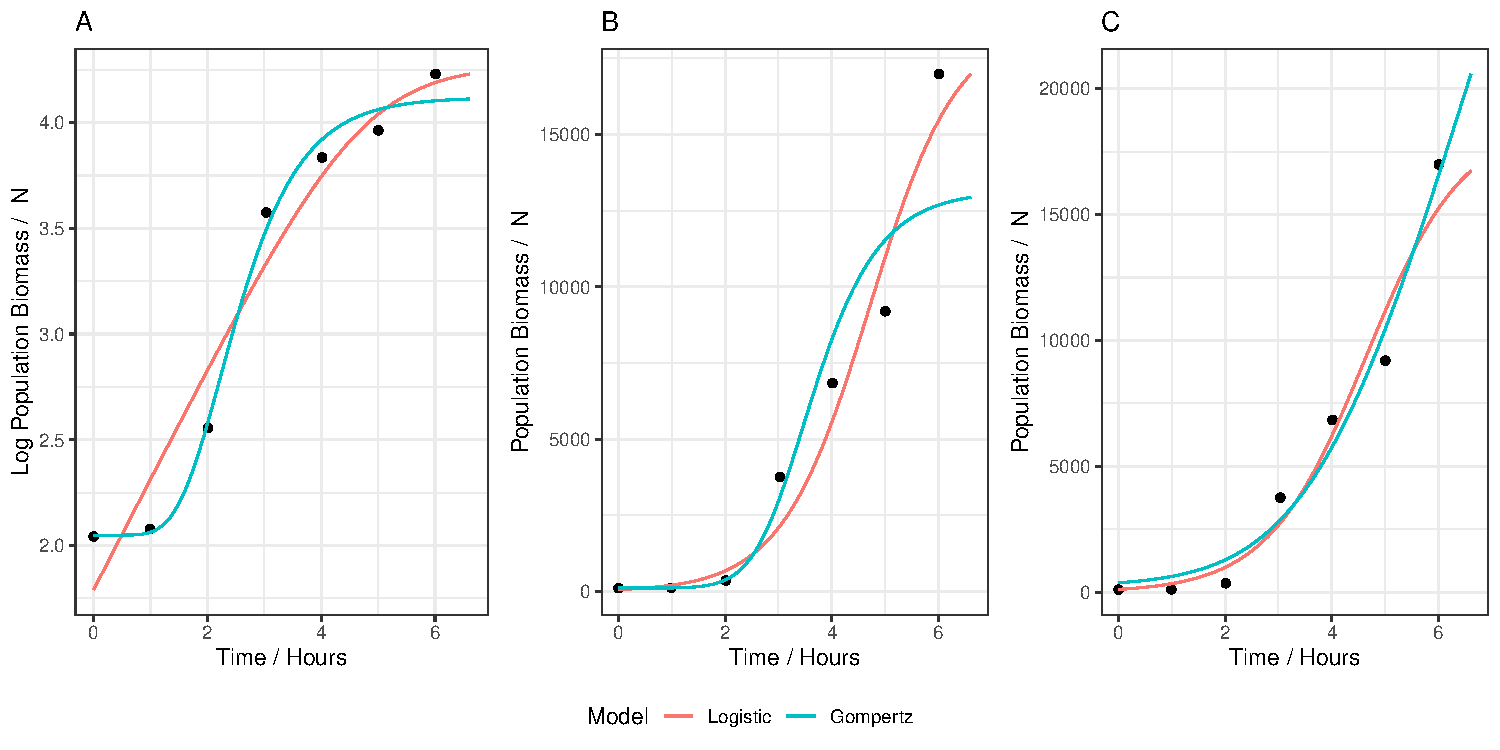
\includegraphics[width=\linewidth]{../results/compare_log_lin_fit.pdf}
        \captionsetup{format=hang}
        \caption{Comparison of: (A) fitting and evaluating modelling in log space. (B) fitting model in log space, evaluating fit in linear space. (C) fitting and evaluating model in linear space. \newline When the models are fit and evaluated in log space, it is clear that the Gompertz model has a better fit. However, if evaluation is done in linear space of these fits, the logistic model appears to have a better fit. This is shown to be invalid, as fitting the models in linear space demonstrates that the Gompertz model can in fact achieve better fits in both spaces.  }
        \label{sup:compare_least_squares}
        \end{figure}
        
        
        \begin{figure}[H]
        \centering
        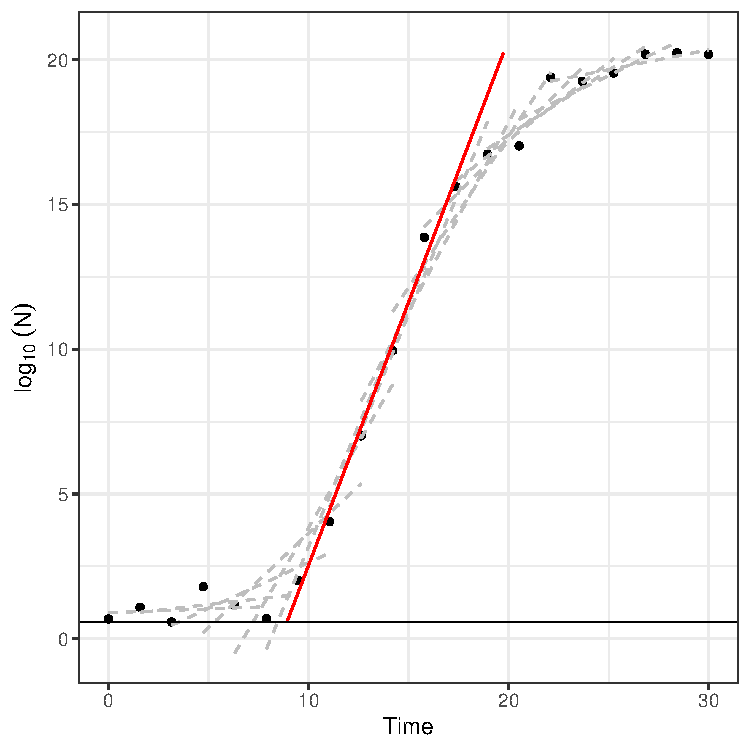
\includegraphics[width=3.5in]{../results/rolling_reg.pdf}
        \caption{Rolling regression was used to produce starting parameters. The regression line with the greatest gradient was selected, with its gradient used as $\mu_{max}$, and its intercept with $N = \min(N)$ used as $t_{lag}$ }
        \label{sup:rolling_regression}
        \end{figure}  
        
        
         \begin{figure}[H]
        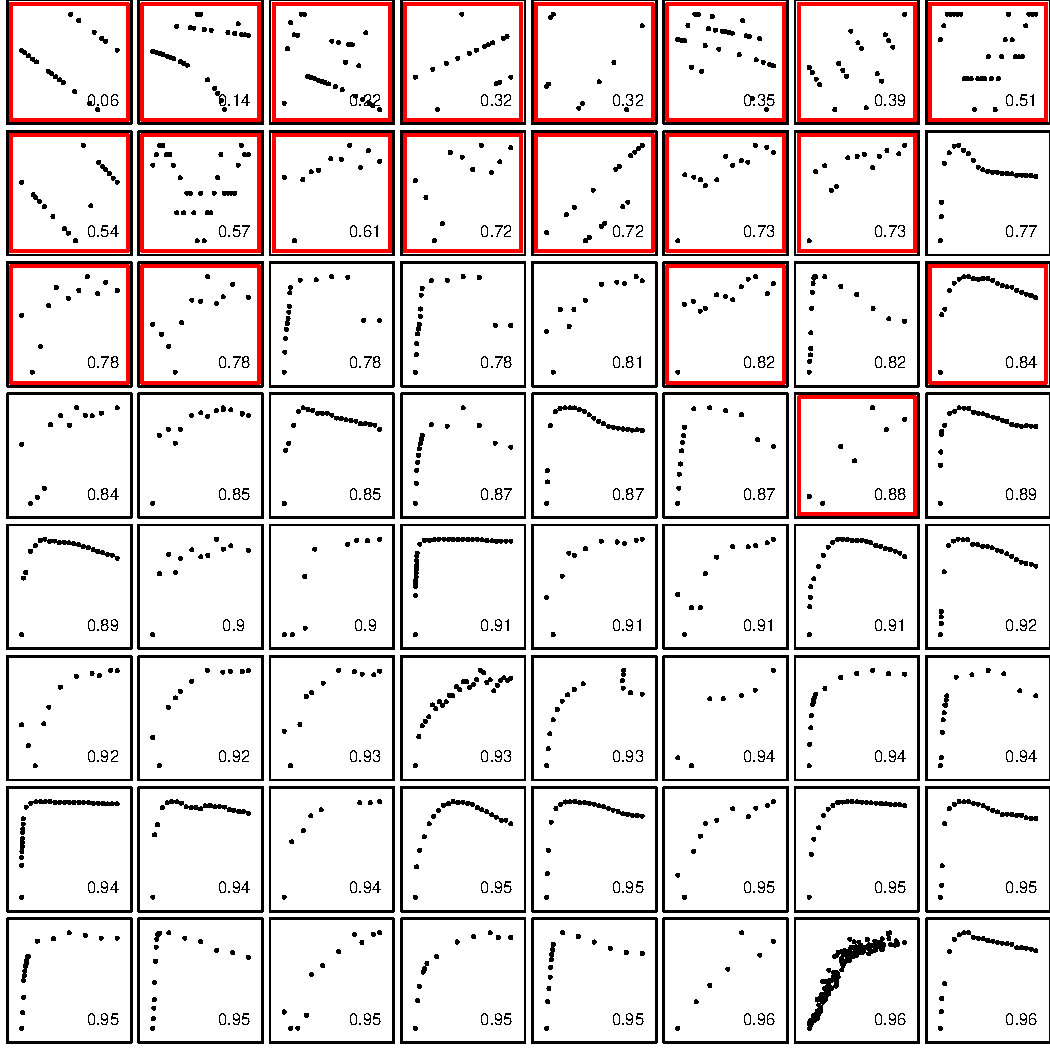
\includegraphics[width=\linewidth]{../results/removed_ids.pdf}
        \caption{The 64 datasets with the lowest maximum R\textsuperscript{2}. Those which were manually removed are highlighted with a red border.}
        \label{sup:removed_ids}
        \end{figure}
        
         \begin{figure}[H]
        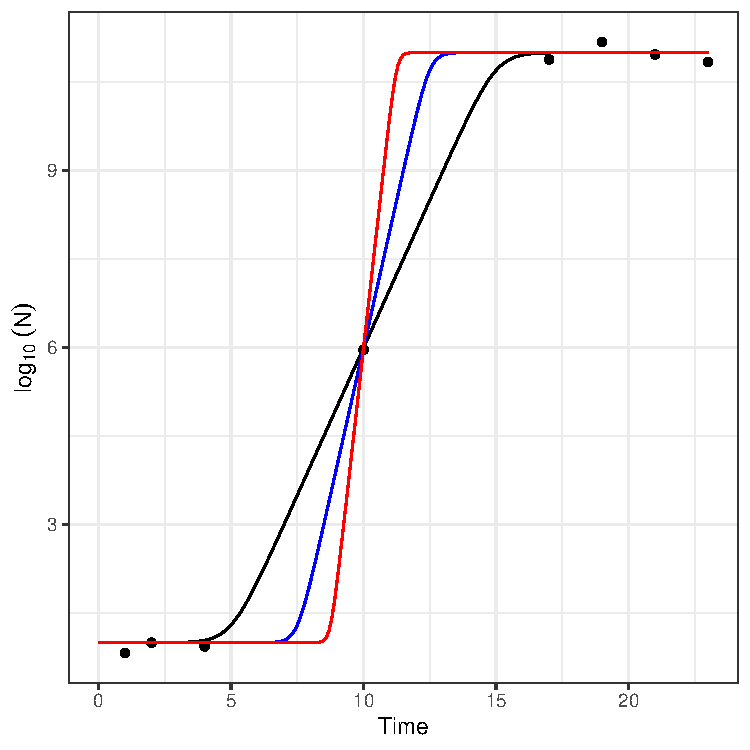
\includegraphics[width=3.5in]{../results/constraint_demo.pdf}
        \centering
        \caption{If there are too few points in the growth phase, $\mu_{max}$ and $t{lag}$ will not be well constrained. Here, we can see that there are infinitely many solutions that can fit equally well to the data as there is only one point in the growth phase. }
        \label{sup:constraint}
        \end{figure}  


         \begin{figure}[H]
         \centering
        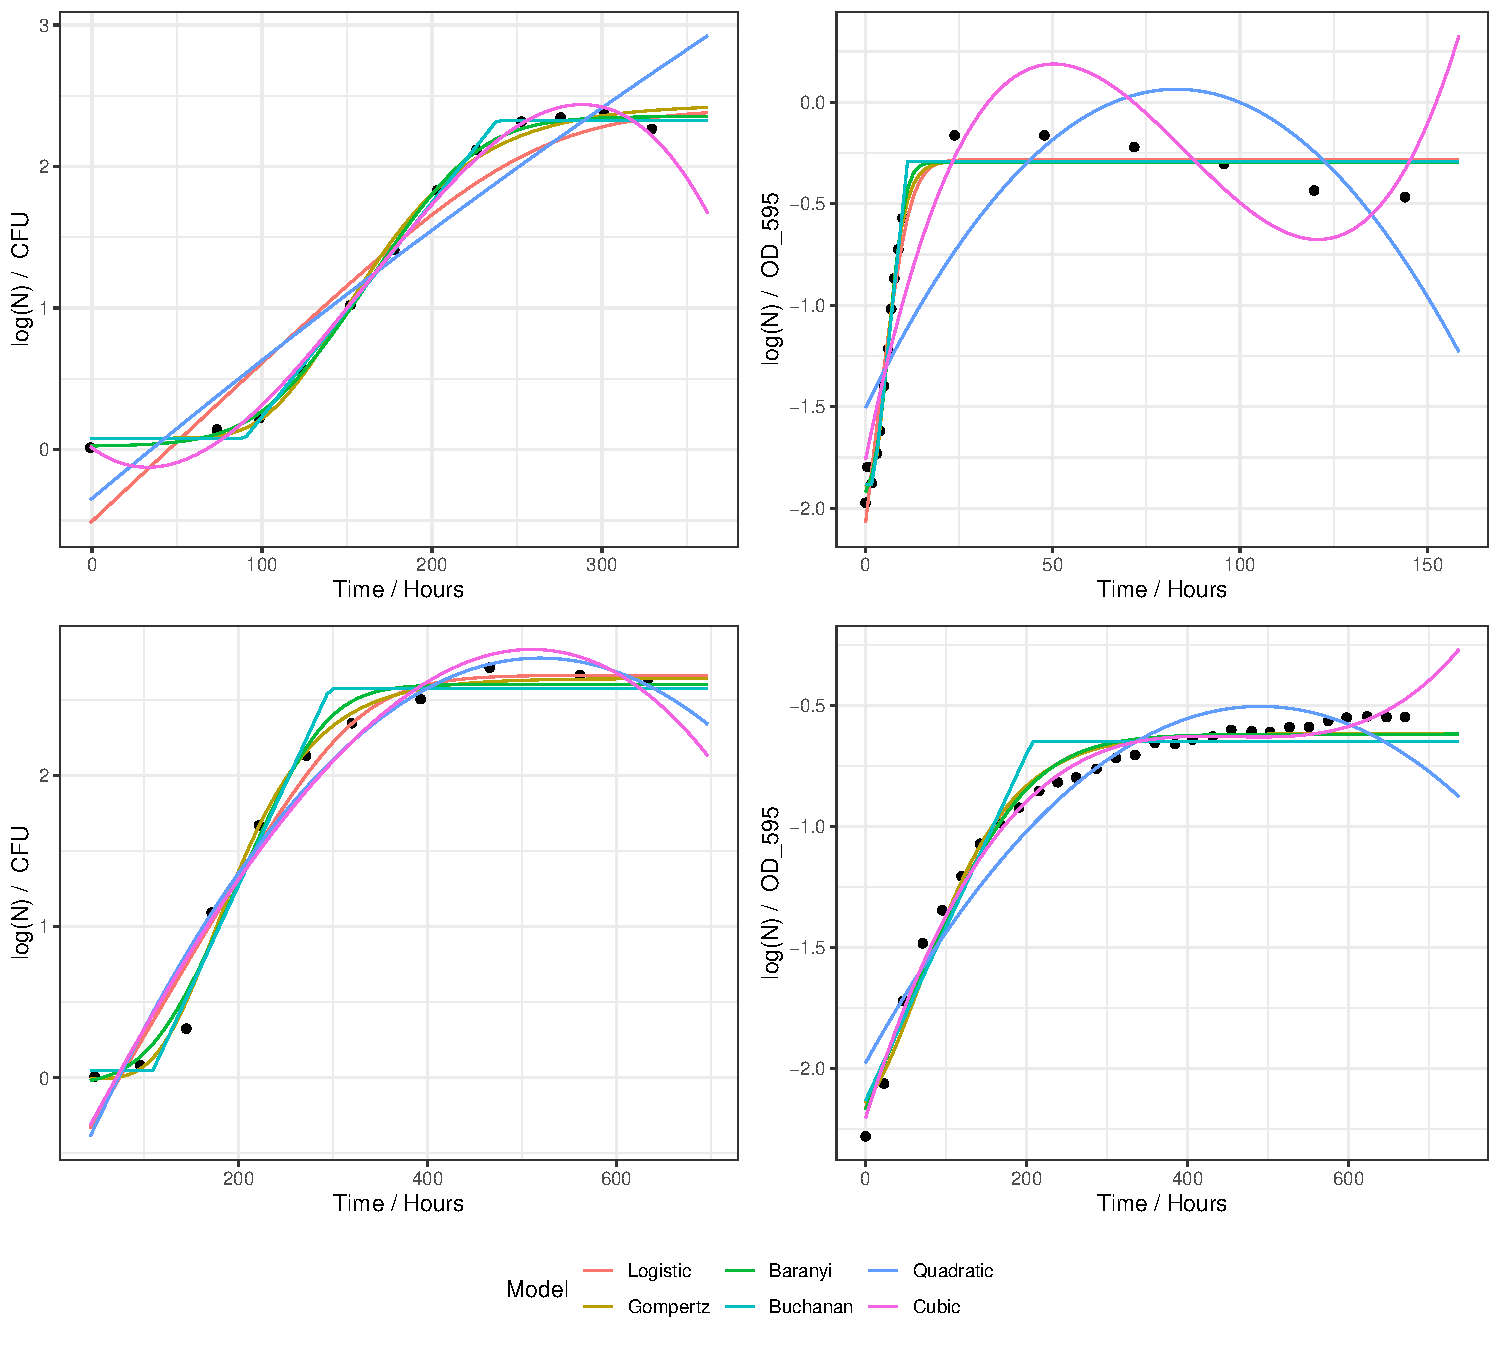
\includegraphics[height=4.5in]{../results/model_fits_linear.pdf}
        \caption{Demonstration of model fits in linear space. Out of 287 data sets, all fits were successful apart from a single fit of the Buchanan model, to a dataset which was removed anyway.}
        \label{sup:model_fits_linear}
        \end{figure}

         \begin{figure}[H]
        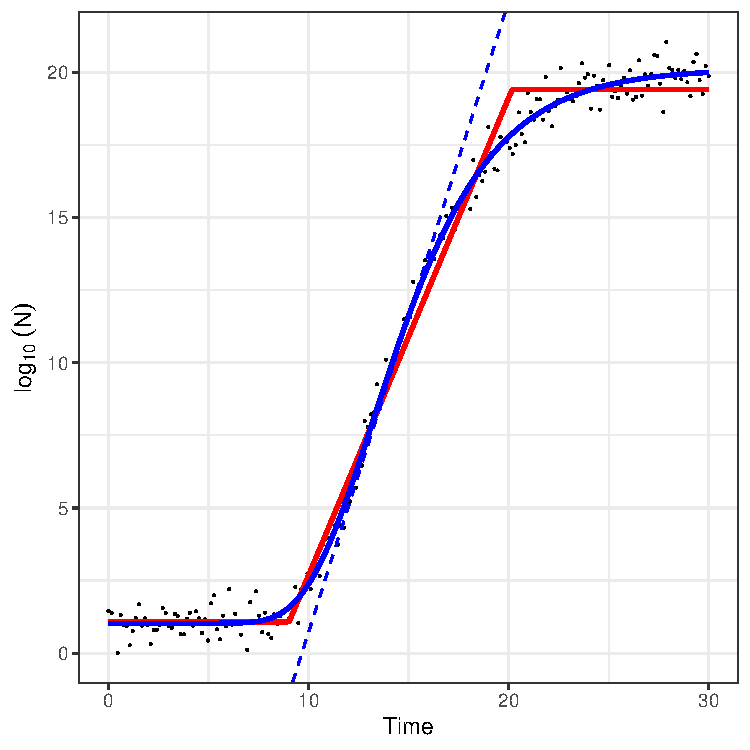
\includegraphics[width=4in]{../results/fit_difference.pdf}
        \centering
        \caption{The Buchanan and Gompertz models are fit to the same hypothetical growth data, which results in smaller $t_{lag}$ and $\mu_{max}$ estimates from the Buchanan model in order to capture the start of the growth phase. By contrast, there is some growth before $t = t_{lag}$ in the Gompertz model.}
        \label{sup:fit_difference}
        \end{figure} 
        
        
         \begin{figure}[H]
        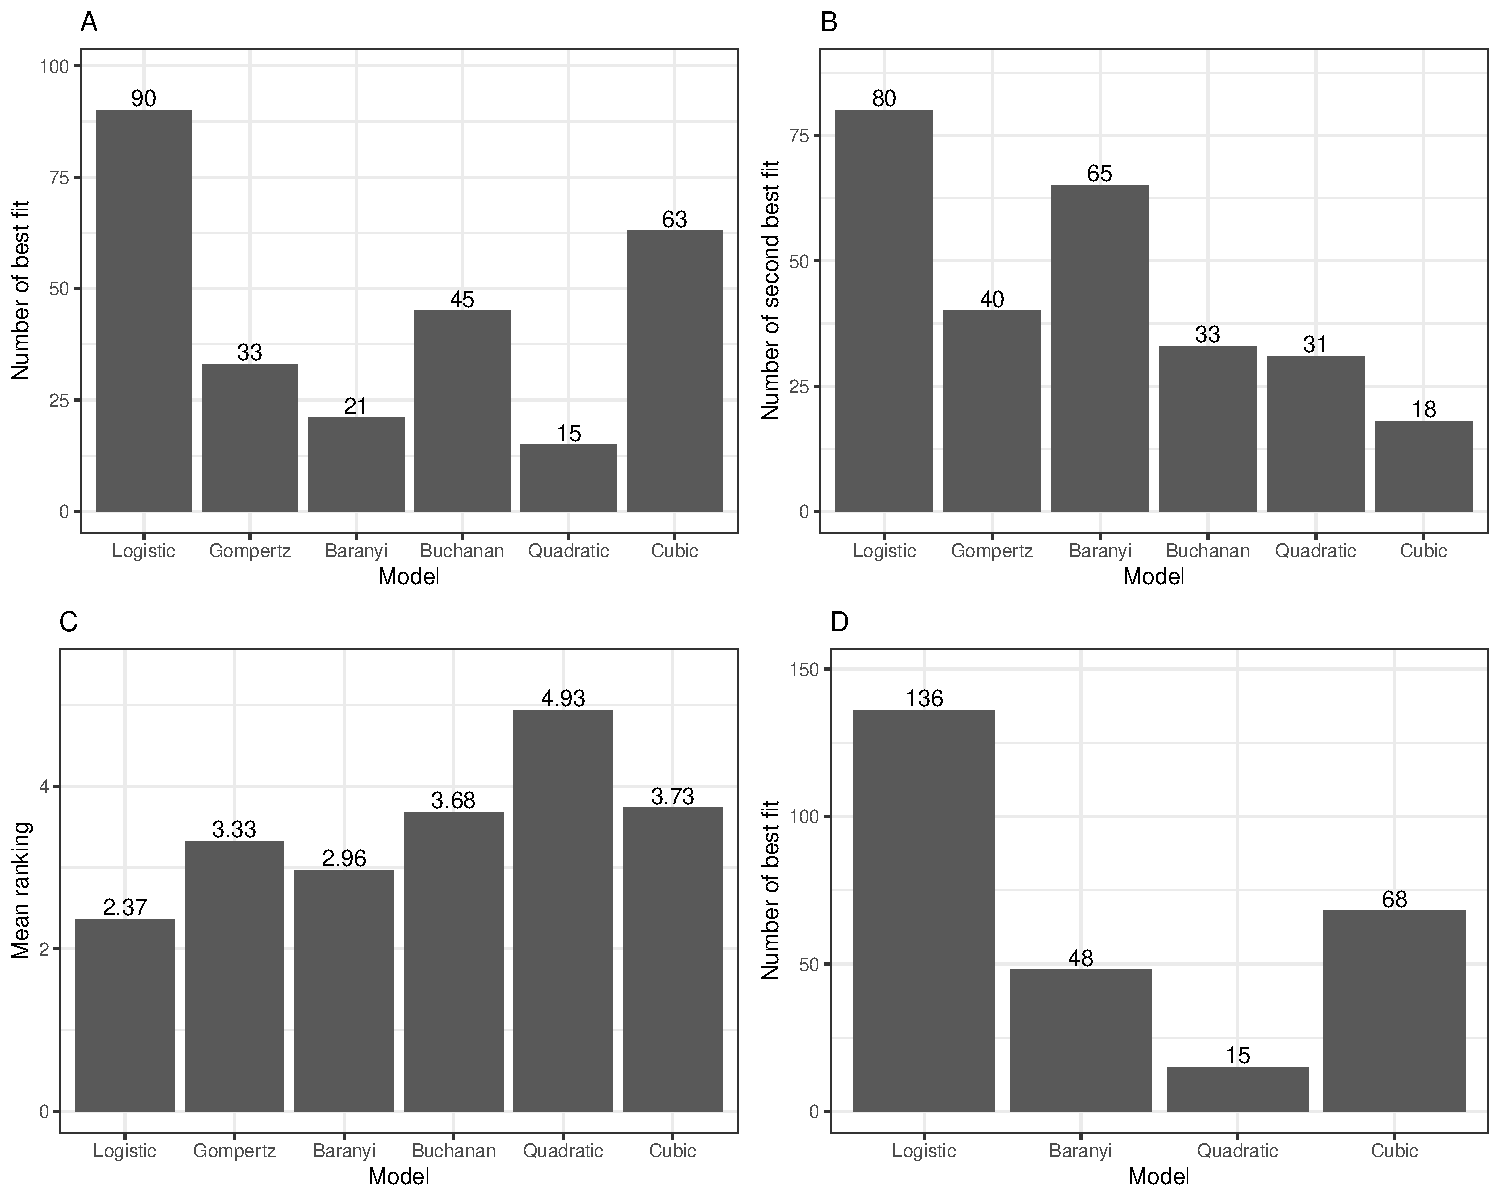
\includegraphics[width=4in]{../results/best_fit_frequency_bar_linear.pdf}
        \centering
        \caption{Plots showing rankings of models in linear space. (A) shows the number of times each model is the best fitting model for a dataset. (B) shows the number of times each model is the second best fitting model for a dataset. (C) shows the mean ranking for each model. (D) shows the number of times each model is the best fitting model for a dataset if we do not consider the Gompertz and Buchanan models.  In linear space, the logistic model performs better than it does in log space, as less emphasis is put on the lag phase.}
        \label{sup:frequency_bar_linear}
        \end{figure} 
        
\begin{table}[H]
\centering
\begin{tabular}{l|llllll}
       & Logistic & Gompertz & Baranyi & Buchanan & Quadratic & Cubic \\ \hline
AIC & 62.3    & 61.8    & 61.3   & 65.5    & 76.3     & 67.7 \\
BIC & 63.8    & 63.8    & 63.3   & 67.5    & 77.8     & 69.7 \\
$A_w$ & 0.213     & 0.174    & 0.158   & 0.178     & 0.0493     &   0.229

\end{tabular}
\caption{Mean AIC, BIC, and Akaike weight values for each model fitted in linear space}
\label{suptable:meanAICBIClinear}
\end{table}




        
        \begin{figure}[H]
        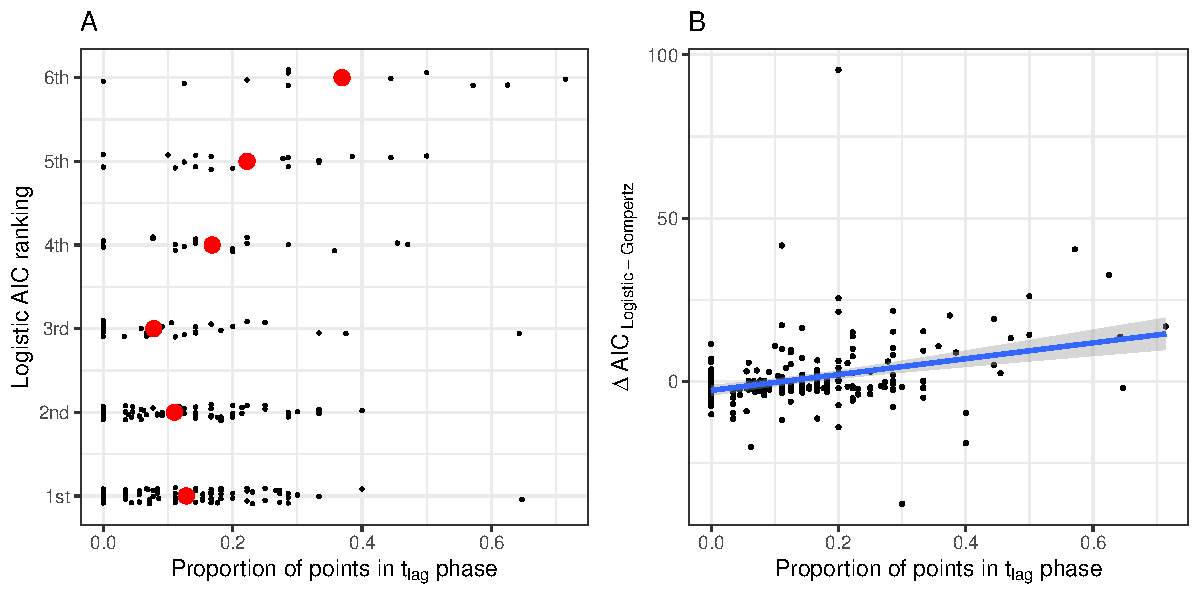
\includegraphics[width=5in]{../results/tlag_vs_logistic_linear.pdf}
        \centering
        \caption{(A) is a plot of proportion of points in the lag phase, against the ranking of the Logistic model by AIC in linear space. (B) shows the difference in AIC score between the Gompertz and Logistic model against this proportion, In both cases, the relationship between Logistic model performance and $t_{lag}$ is much weaker than in log space. The difference in AIC between Logistic and Gompertz decreases by 2.4 for every increase in lag phase proportion by 0.1 (in contrast to 6.9 for log space)}
        \label{sup:tlag_logistic_linear}
        \end{figure} 
        
         \begin{figure}[H]
        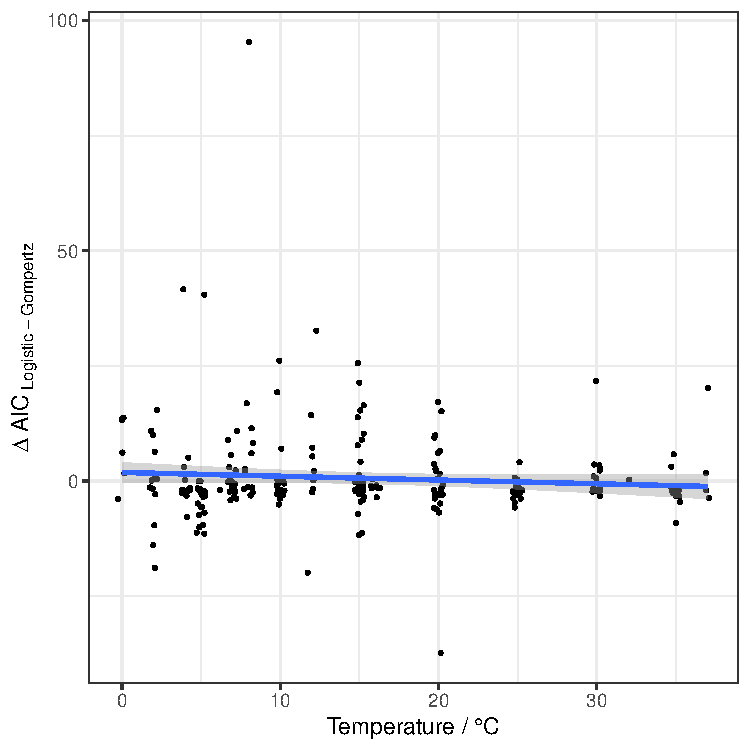
\includegraphics[width=3in]{../results/logistic_vs_gompertz_temp_linear.pdf}
        \centering
        \caption{$\Delta_{\text{Logistic - Gompertz}}$ no longer has a statistically significant relationship with temperature when models are fit in linear space. This implies that the fit of the Logistic model does not become any weaker realtive to thegompertz model as temperature increases.}
        \label{sup:logistic_temp_linear}
        \end{figure} 
        
        \begin{figure}[H]
        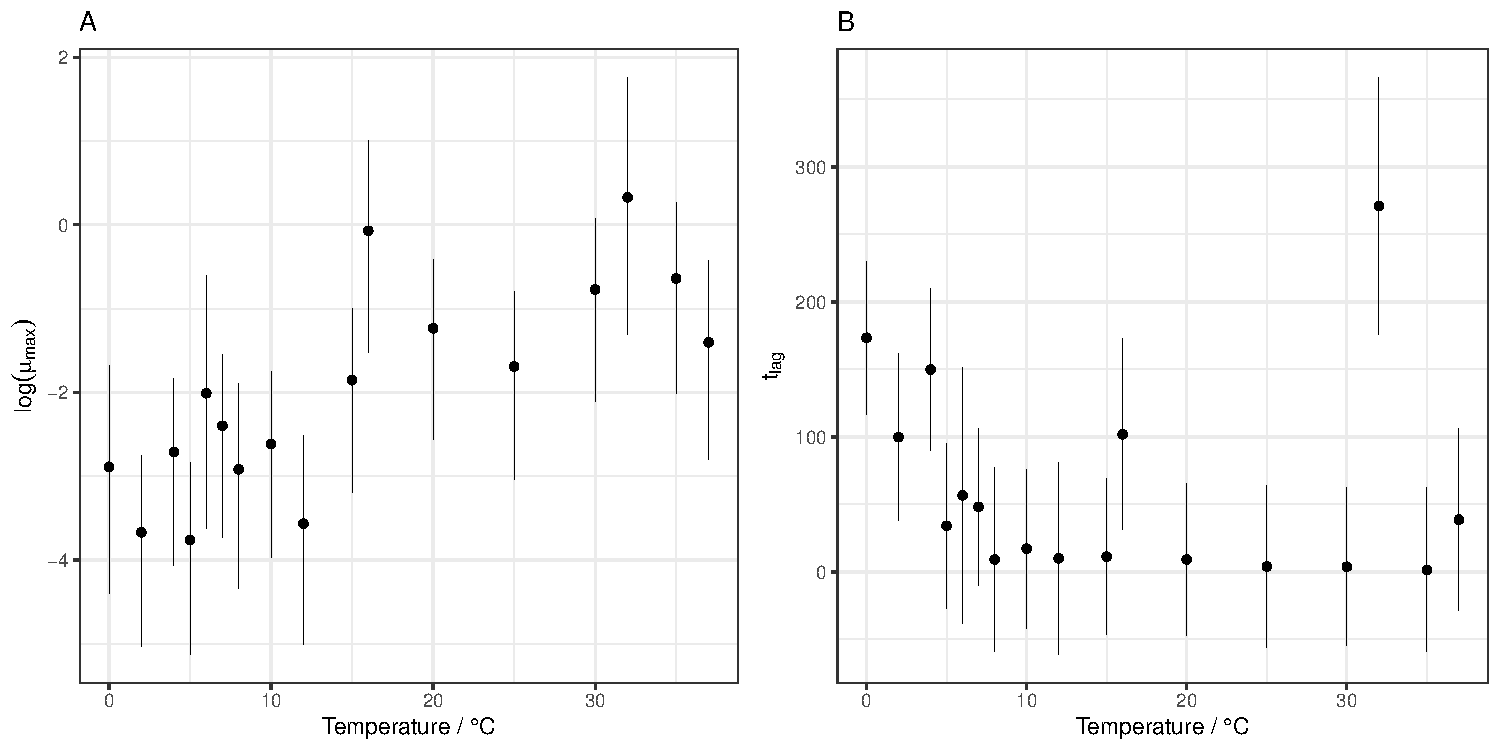
\includegraphics[width=\linewidth]{../results/tlags_linear.pdf}
        \centering
        \caption{The broad patterns of $\mu_{max}$ and $t_{lag}$ are the same when model fitting is in linear space, but the confidence intervals are much broader.}
        \label{sup:params_linear}
        \end{figure} 
        
        
    \bibliographystyle{ieeetr}
    \bibliography{write_up}

\end{document}
}

\newcommand{\beginsupplement}{%
        \setcounter{table}{0}
        \renewcommand{\thetable}{S\arabic{table}}%
        \setcounter{figure}{0}
        \renewcommand{\thefigure}{S\arabic{figure}}%
}


\setcounter{secnumdepth}{0}
\begin{document}

    \begin{titlepage}
	\centering
	
\includegraphics[width=0.5\textwidth]{../data/imperial.png}\par\vspace{1cm}
	\vspace{2cm}
	{\scshape\Large\bfseries Recommendations for Fitting Microbial Growth Models\par}
	\vspace{2cm}
	{\Large Sam Turner\par}
	\vspace{0.5cm}
	{\Large March 2020 \par}
	\vspace{0.5cm}
	{\Large\itshape Computational Method in Ecology and Evolution MSc\par}
	\vspace{0.5cm}
	 \wordcount words 
	\vfill

	\vfill
    
    \newpage
    \end{titlepage}
    

    \begin{abstract}
   Modelling of microbial growth is vital for developing food preservation measures to decrease food waste. By fitting a range of mechanistic and phenomenological models to a large dataset of 305 growth curves, I demonstrate that temperature has a major impact on microbial population dynamics. I also examine how methodological choices can influence the results of model fitting studies, including demonstrating that the choice of model can systematically bias parameter estimates to the extent that they become incomparable for meta-analysis. Improvements in the resolution of parameter estimates when models are fit in logarithmic space relative to linear space model fitting are also reported. These findings result in recommendations for microbial modelling methodology, particularly when data are aggregated across sources.
\end{abstract}
\tableofcontents
\begin{linenumbers}
    \section{Introduction}
    
    There is great interest in modelling the growth of microbial populations, in order to understand their response to external variables \cite{zwitmodelling}. This allows prediction of shelf lifes and optimisation of preservation methods. In this project, I address four questions:    

\begin{enumerate}
  \item Which models best describe microbial population growth, and how does this vary with temperature?
  \item How does temperature affect microbial growth?
  \item How does choice of model affects parameter estimates?
  \item Does the choice to fit models in linear or logarithmic space affect results?
  \end{enumerate}


I addressed these by fitting mechanistic and phenomenological models to a dataset of 305 digitised growth curves. Each mechanistic models describes the growth curve with a mathematical relationship representing a hypothesis about the dynamics of microbial growth \cite{Buchanan}, so is parameterised with meaningful biological quantities. In contrast, the phenomenological models are simply convenient mathematical functions used to describe patterns in the data, and are used as a neutral comparison for the mechanistic models. By comparing the fit of the mechanistic models to each other, and to the phenomenological models, support for the underlying biological hypothesis can be determined. I also examine the effect of temperature, both on the relative support for the models, and on the growth rate and lag time of microbial populations, as these play a central role in food spoilage. 

By comparing parameter estimates between models, and comparing results from fits in logarithmic and linear space, I also investigate how methodological choices can impact results. In particular, I was interested in whether differences in methodology could invalidate comparison of parameter values from different sources in meta-analyses.

\subsection{The Mechanistic Models}

The mechanistic models can be split into three four-parameter models, and the three-parameter logistic model. The four-parameter models split the growth curve into a lag phase, exponential phase, and stationary phase, with the logistic model discarding the lag phase.

\paragraph{Logistic}
The logistic model \cite{logisticVel1, logisticVel2} assumes that the microbial population immediately starts growing exponentially, with its growth rate falling towards zero as population size approaches a carrying capacity. This is described by the logistic differential equation:

\[ \frac{\mathrm d N}{\mathrm d t} =  \mu_{max}N(1-N)  \]

With solutions:

\[ N_t =   \frac{N_0  N_{max} e^{\mu t}}{N_{max} + N_0 (e^{\mu t} - 1)} \]


\subsubsection{Four-parameter models}

These models parameterise the sigmoidal growth curve with minimum and maximum population sizes, maximum growth rate, and a time lag before the population starts growing (illustrated in Figure \ref{fig:4_param_demo}). As such, the rate of growth and length of the lag phase can be independently varied (Figure \ref{fig:parameter_variation_demo})

        \begin{figure}[H]
        \centering
        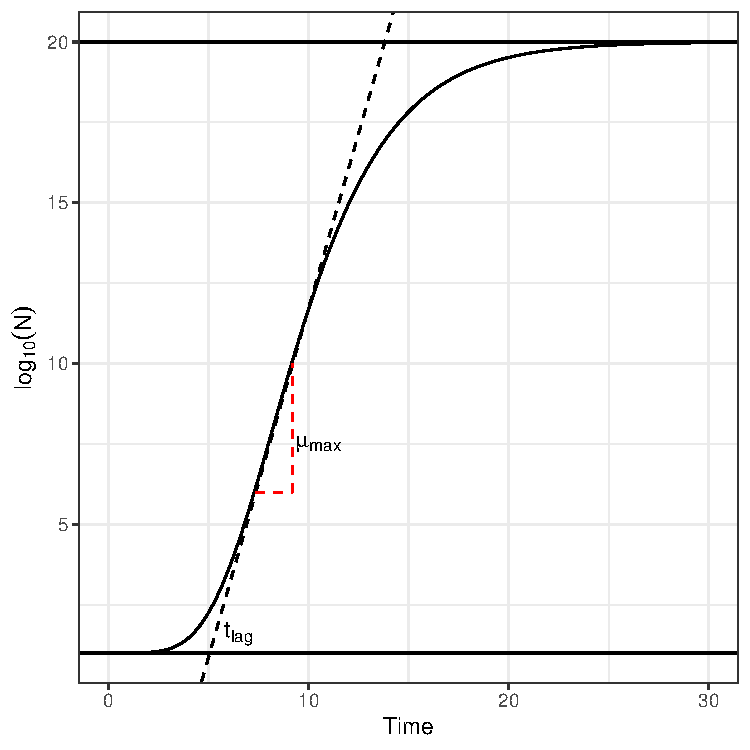
\includegraphics[width=4in]{../results/4_param_demo.pdf}
        \caption{Illustation of $\mu_{max}$ and $t_{lag}$ parameters. $\mu_{max}$ is the maximum gradient of the growth curve, and $t_{lag}$ is the intercept between this tangent line and the line $N = N_0$}
        \label{fig:4_param_demo}
        \end{figure}


        \begin{figure}[H]
        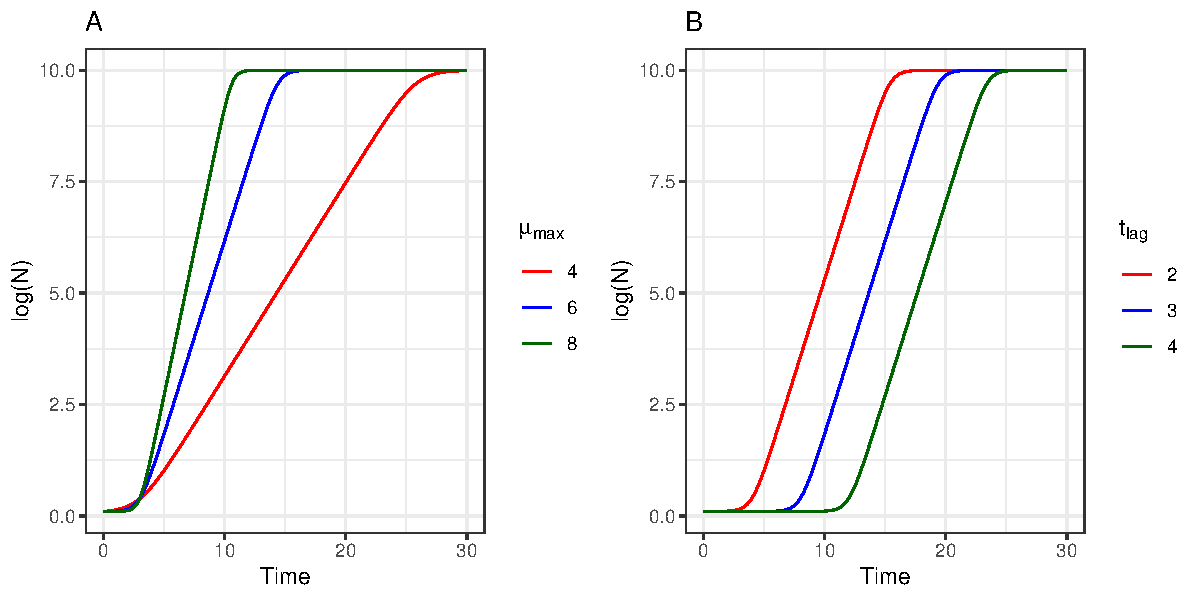
\includegraphics[width=\linewidth]{../results/tlag_rmax_demo.pdf}
        \caption{ $(A)\mu_{max}$ and (B) $t_{lag}$ parameters can be varied independently to control the rate of microbial growth, and the duration of the lag phase.}
        \label{fig:parameter_variation_demo}
        \end{figure}



\paragraph{Buchanan}
The Buchanan model \cite{Buchanan} is the simplest implementation of this, with a growth rate of zero during the lag and stationary phases, which surround a period of exponential growth:

  \[
    log(N_t) = \begin{cases}{}
        N_0 & \quad \text{if } t\leq t_{lag}\\
        N_0 + \mu_{max} \cdot (t - t_{lag}) &  \quad \text{if } t_{lag}\leq t\leq t_{max}\\
        N_{max} &  \quad \text{if } t\geq t_{max}
        \end{cases}
  \]

\paragraph{Gompertz}

The Gompertz model \cite{Gomp, zwitmodelling} describes a sigmoidal growth curve with a gradual transition into and out of the exponential phase. The Gompertz model has been popular for microbial population modelling, as it has empirically been found to fit well in a wide range of circumstances \cite{MicrobialGrowth}. However, it should be noted that its derivation does not have a mechanistic basis in microbial growth modelling \cite{EstBaranyi}, but rather in describing human mortality rates \cite{Gomp}. 

  \[log_{10}(N_t) = N_0 + (N_{max} - N_0)  e^{-e^{ \frac{\mu_{max} ~ \cdot ~ e  ~ \cdot ~ (t_{lag} - t)}{ (N_{max} - N_0) ~ \cdot ~ log(10)} + 1} }\]
  
  
\paragraph{Baranyi}

The Baranyi model is an attempt to formulate a truly mechanistic model for microbial population growth \cite{BaranyiOriginal, zwitmodelling}, explicitly modelling the internal physiological state and external environmental conditions of the cell. This produces a more flexible model, which can be applied to model population growth curves in time-varying environmental conditions. Here,  we use a version of the model in which conditions are homogenous, with the curvature parameter into the exponential phase $\nu$ set to $\mu_{max}$, and curvature parameter out of the exponential phase $m$ set at an empirical estimate of 1:

\[ log_{10}(N_t) = N_{max} + log_{10}(\frac{-1 + e^{\mu_{max} \cdot  t} + e^{\mu_{max} \cdot t_{lag}  } }{ -1 + e^{\mu_{max} \cdot t}  + e^{\mu_{max} \cdot t_{lag}} \cdot 10^{N_{max}-N_0}}) \]


        \begin{figure}[h]
        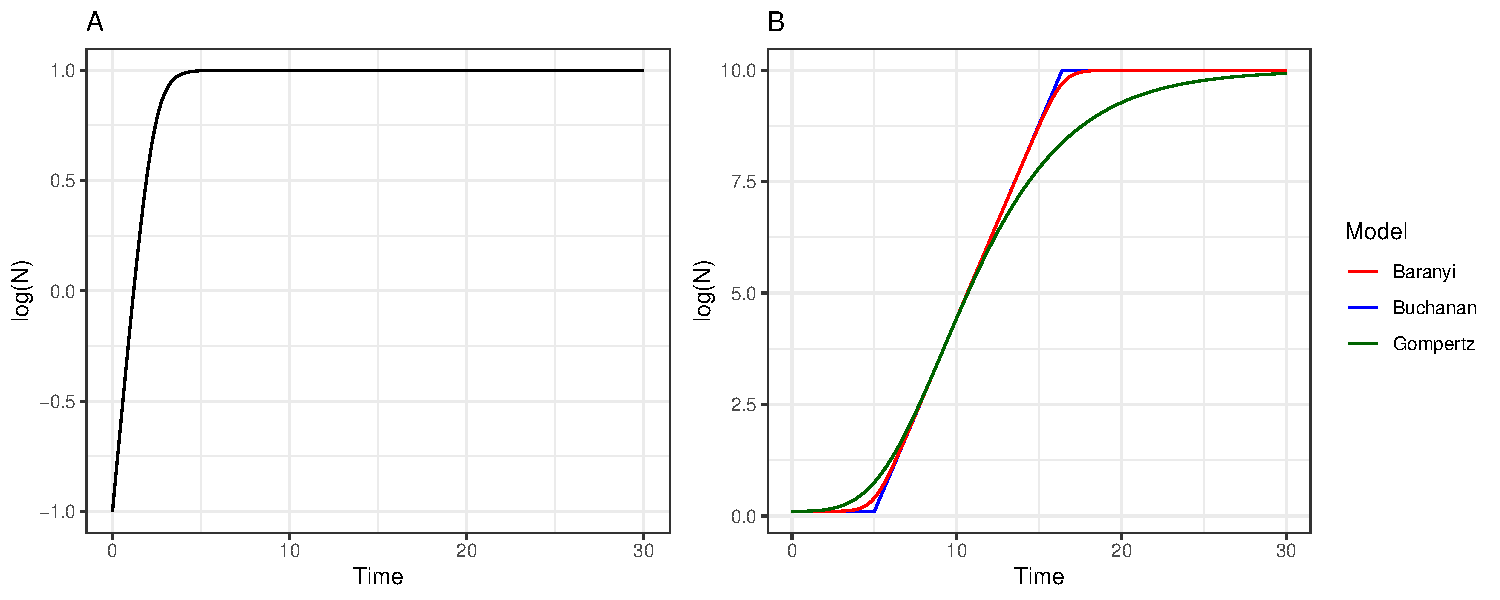
\includegraphics[width=\linewidth]{../results/model_demo.pdf}
        \captionsetup{format=hang}
        \caption{Demonstration of the shape of the 4 mechanistic models, plotted in log space. The logistic model (A) immediately starts growing at its maximum growth rate, whilst the three four-parameter models (B) have growth phases that transition into the exponential phase}
        \label{fig:models_demo}
        \end{figure}

\subsection{Phenomenological models}
As controls, I decided to fit quadratic and cubic polynomials to the data:
\paragraph*{Quadratic} $ N_t = at^2 + bt + c $
\paragraph{Cubic} \quad \quad $ N_t = at^3 + bt^2 + ct + d $


   \section{Methods}
   
   \subsection{Data}
   
\paragraph{Data sources}
The provided microbial growth data contained 305 time series, digitised from graphs in 10 papers from the microbial growth literature. The data set contained time series from 47 different species, 18 media, and 17 temperatures, with population size measured in 4 different units. However, the data from one citation \cite{discarded} clearly had incorrect time values, with times extending to 13,000 hours. I removed the data from this citation as there was not a clear correct transformation to produce the correct times, leaving 287 time series for analysis.

\paragraph{Log transformation}
As explained below, I decided to fit the model to $log_{10}(N)$ as well as to linear data. In 5/287 data sets, there were negative population counts due to numerical error in growth curve digitization. One value of approximately -668 was removed, whilst other negative values were greater that -10\textsuperscript{-2}; in these cases, I transformed increased population sizes for that time series by the minimum population size in the time series, discarding the minimum value of 0 before taking the logarithm.  

\paragraph{Time transformation}
I transformed each time series to start at $t = 0$ when fitting the four-parameter models, as model fits were clearly suboptimal without this transformation. Since $t_{lag}$ directly transforms the curve along the t-axis, $t_{lag}$ could be adjusted back to obtain model parameters which fit the untransformed time series. 

\subsection{Model Fitting}
When fitting the models, I used a least squares approach, both to log\textsubscript{10} transformed data, and to the original linear data (Figure \ref{sup:compare_least_squares}). This required exponentiating the four-parameter models to predict linear population size, and taking the logarithm of the logistic model to predict logarithmic population size. As such, the parameters of the four-parameter models remained in logarithmic space, and the parameters of the Logistic model in linear space. 

Due to the advantages presented in Results, I analysed parameter estimates from the log-fitted models (although linear fit results are presented in the Supplementary Figures), also choosing not to linearise residuals as this resulted in non-sensical fits (demonstrated in Figure \ref{sup:compare_least_squares}). These fits can be explained by the fact that, in general:
\[log(f(x) ) \neq f(log(x))\]
This means minimising errors in logarithmic space does not result in minimised errors in linear space, so evaluating fit in linear space does not capture the best possible fit for each model, (Figure \ref{sup:compare_least_squares}).

\subsubsection{Fitting linear models}

The two polynomial phenomenological models are linear in their parameters, so were fitted using Ordinary Least Squares with the lm() function in R \cite{R}.

\subsubsection{Fitting non-linear models}

The mechanistic models are non-linear, so are fitted using an optimisation approach. The nlsLM function in the minpack.lm \cite{minpack} package uses the Levenberg-Marquardt algorithm to optimise initial values to determine best fitting parameter values for a specified model. If initial values are far from the optimal parameters, it is likely that the optimisation will not converge, or will converge to very suboptimal parameters. It is therefore important to estimate reasonable starting values.

\paragraph{Estimating parameter values}
N\textsubscript{min} and N\textsubscript{max} were set as the minimum and maximum observed population size respectively. $\mu_{max}$ and $t_{lag}$ estimates were determined using a rolling regression (Figure \ref{sup:rolling_regression}), which computed the regression line for all sets of 5 adjacent data points. The regression line with the greatest gradient was selected, with the gradient taken as an estimate of $\mu_{max}$, and the $t$ value at the intercept between this regression line and $N = \min(N)$ taken as the $t_{lag}$ estimate. This was repeated in both logarithmic and linear space to provide parameter values for Logistic and four-parameter models.


\paragraph{Multiple fit attempts}
Despite well chosen initial values, models often fail to converge, or converge to poorly fitting parameter values. To increase the proportion of models which fit, and ensure that I find parameter values nearer the global optimum, I used a grid search to explore a range of initial parameter values. For each parameter, I chose linearly spaced samples from a range surrounding the estimate of that parameter value, and fitted a model for every combination of these parameter values. For example, if I take 3 samples for each of $N_0$ and $N_{max}$, and 5 for $t_{lag}$ and $\mu_{max}$, I fit $3 \times 3 \times 5 \times 5 = 225$ models. From the model fits that converge, I select the model with the smallest RSS. If none converge, I randomly sample parameter values with normally distributed noise around my parameter estimates until a model fits, or until there have been 1,000 failed attempts. 

Using this method, I was able to fit all 287 data sets for the Logistic, Gompertz, and Baranyi models in both linear space and logarithmic space. In linear space, there was one failed fit for the Buchanan model, and in log space there were two failed fits for the Buchanan model.


\subsection{Filtering}
Some data sets show no pattern of population growth, or have too few points in the growth phase to constrain the $mu_{max}$ and $t_{lag}$ parameters. I visualised the 64 data sets with the lowest maximum R\textsuperscript{2} value, removing 20 with no meaningful growth pattern or visibly little constraint (Figure \ref{sup:removed_ids}). For parameter estimate analysis, I further filtered out datasets with fewer than 2 points in the growth phase (Figure \ref{sup:constraint}) by counting the number of points with a time value within the predicted exponential phase, as determined using Akaike weighted parameter values. This removed a further 57 data sets, leaving 210 data sets.


\subsection{Model Selection}

Model fit was assessed using AIC \cite{AIC} and BIC \cite{BIC}. With the assumption of normally distributed errors, and simplification to remove constants, these are:
\[\text {AIC}  = 2k + n\log(RSS)\]
\[\text {BIC} = n\log{\frac{RSS}{n}} + k\log{n}\]


Both AIC and BIC balance fit against model complexity, allowing direct comparison of fit for models with differing numbers of parameters. However, BIC has the disadvantage of making a number of unrealistic assumptions about the true model: that it exists, is in the model set, and has equal prior probability to other models. Additionally, the fact that AIC is based in Kullback–Leibler information theory means that standardised model likelihoods - Akaike weights - can be calculated to naturally compare model support and allow model averaging \cite{Omland, ModelSelection}.


\subsection{Parameter Estimation}

Parameter estimation was performed using Akaike weights, which produce a single parameter estimate from a family of models \cite{ModelSelection}, weighted by the model’s relative likelihood.
With $\text{AIC}_{best}$ being the lowest observed AIC values for a dataset, $\Delta_{AIC}$ values are calculated with:
\[ \Delta_i = \text{AIC}_i - \text{AIC}_{best} \]

The Akaike weight for the $i^{th}$ model is then:
\[ w_i = \frac{e^{-\frac{1}{2}\Delta_i }} { \sum_{r = 1}^{r = R}  e^{- \frac{1}{2}\Delta_r }}\]

The Akaike weighted parameter estimate for $\theta$, with weights $w_i$ and individual model parameter estimates $\theta_i$ is:
\[\theta_w = \sum_{i = 1}^{i = I}\theta_i * w_i\]


\subsection{Statistical Analysis}

I ran linear regressions of $\Delta_{\text{Logistic - Gompertz}}$ against temperature, and $\Delta_{\text{Logistic - Gompertz}}$ against proportion of points in the lag phase, using lm() in R \cite{R}. Their diagnostic plots were examined to confirm the suitability of a linear model.

I ran a mixed effects model of $\mu{max}$ against temperature, and of $t_{lag}$ against temperature, with species and medium used as random effects in each case. Again, diagnostic plots were used to confirm that residuals were homogeneous across the fitted values.

I ran a paired t-tests for $\mu_{lag}$ and $t_{lag}$ between the each pair of four-parameter models, and between linear and logarithmic space fits, to check for systematic differences in parameter estimates. I check for normality of differences by plotting histograms of these differences.  

\subsection{Computing Tools}
\paragraph{R 3.6.1 \cite{R}} was used for initial data preparation script, model fitting, analysis, and figure preparation. R was chosen because the native data structures are naturally suited to this type of data, and support of vectorised operations makes the code cleaner than it would be in Python. I used R for my multi-start method to fit models over a range of initial parameter values because of the efficiency of non-linear least squares model fitting in the minpack.lm package. \textbf{minpack.lm \cite{minpack}} was used for non-linear least squares model fitting using the more robust Levenberg-Marquardt algorithm (relative to Gauss-Newton). \textbf{ggplot2 \cite{gg}} was used to create high quality graphics. \textbf{dplyr \cite{dplyr}} was used for data wrangling. \textbf{lme4 \cite{lme4}} was used to fit linear mixed models. \textbf{toOrdinal \cite{tO}} was used for annotations.

\paragraph{Python 3.7.4 \cite{python}} was used for calculation of initial values. \textbf{pandas \cite{pd}} was used for dataframes in Python. \textbf{matplotlib \cite{plt}} was used to create graphics in Python. \textbf{SciPy \cite{numpy}} was used to fit linear regressions for the rolling regression. \textbf{NumPy \cite{numpy}} was used for efficient arrays.

\paragraph{bash 3.2} was used to write scripts tying other elements of the project together.

\paragraph{\LaTeX } was used for compilation of this write-up.
\section{Results}

\subsection{Model fitting is highly successful}
Taking the best fitting model from a range of initial parameter values was very effective, with all models converging to every data set when those with no discernible growth pattern were removed, and only 3 unsuccessful fits otherwise (2293 / 2296 successful non-linear fits overall). Model fits were visually inspected, and found to describe the data well (Figure \ref{fig:model_fits} for logarithmic fits, Figure \ref{sup:model_fits_linear} for linear fits). For the reasons expanded on in the Discussion, I present the results obtained from fitting models in logarithmic space first, before examining the results from linear space fits at the end of this section.

         \begin{figure}[H]
         \centering
       	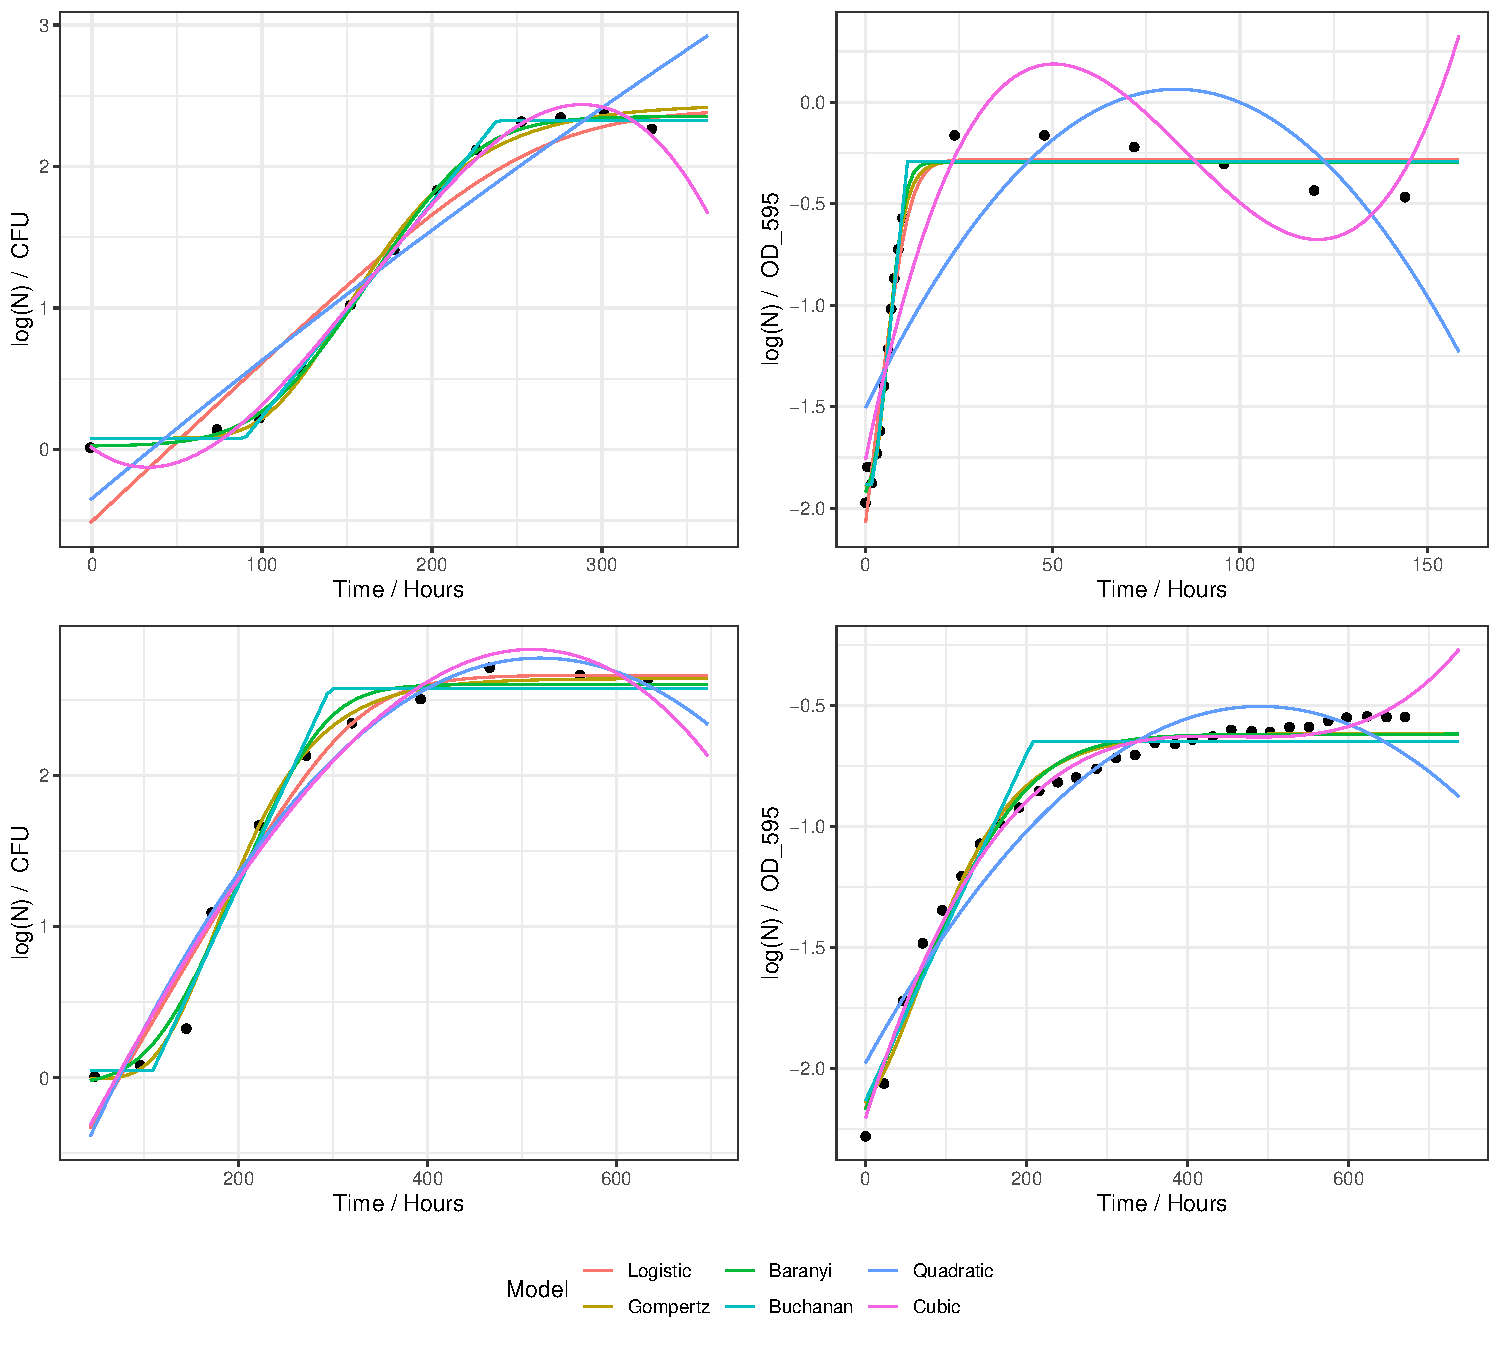
\includegraphics[height=4.5in]{../results/model_fits.pdf}
        \caption{Demonstration of model fits in log space. Out of 287 data sets, all fits were successful apart from two fits of the Buchanan model, to datasets which were removed anyway. }
        \label{fig:model_fits}
        \end{figure}

\subsection{Gompertz and Baranyi are best supported}

The Gompertz model and Baranyi model are both well supported by the data. The Gompertz model most frequently has the lowest AIC (Figure \ref{fig:bestbars} A), and has the highest mean Akaike weight (Figure \ref{AWdist} and Table \ref{tab:meanAICBIC}). However, the Baranyi model has a lower mean ranking (Figure \ref{fig:bestbars} C), and lower mean AICs and BICs. (Table \ref{tab:meanAICBIC}). It appears that the Baranyi model is a consistent good fit to the data, achieving the lowest mean AIC despite relatively rarely being the best fitting model - as evidenced by it placing second for nearly half of the datasets (Figure \ref{fig:bestbars} B).



        \begin{figure}[H]
        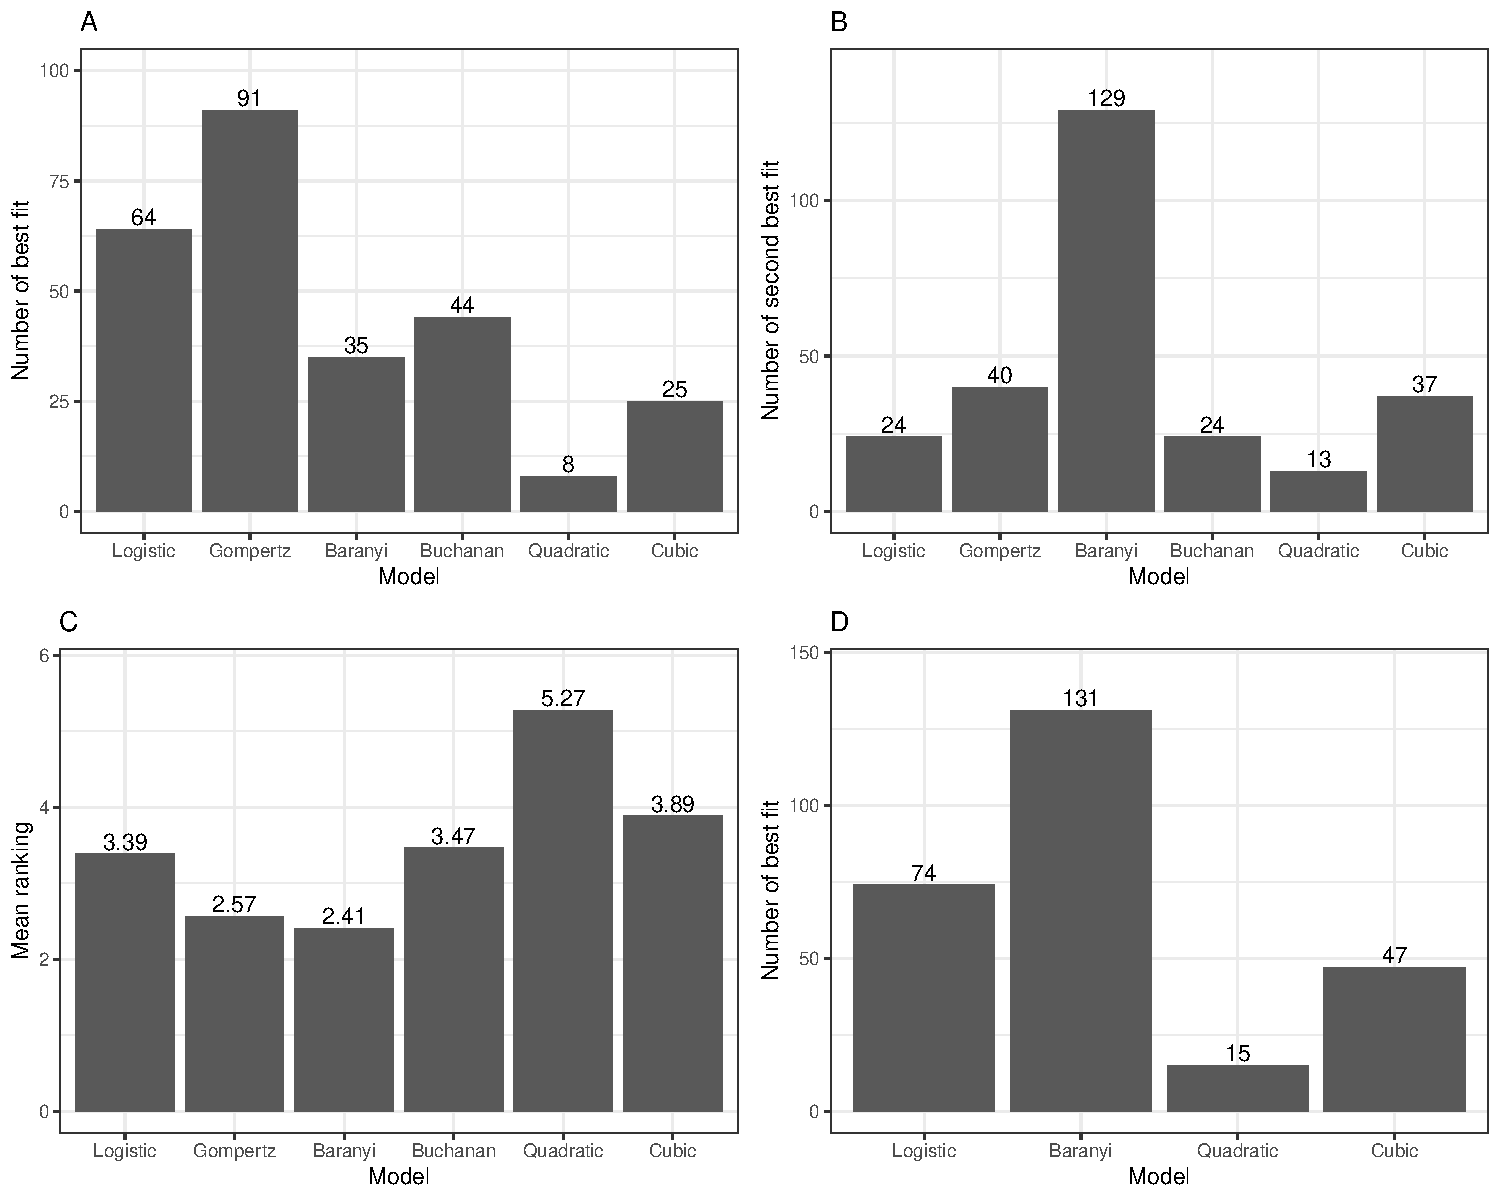
\includegraphics[width=\linewidth]{../results/best_fit_frequency_bar.pdf}
        \caption{Plots showing the rankings of models in logarithmic space. (A) shows the number of times each model is the best fitting model for a dataset. (B) shows the number of times each model is the second best fitting model for a dataset. (C) shows the mean ranking for each model. (D) shows the number of times each model is the best fitting model for a dataset if we do not consider the Gompertz and Buchanan models. }
        \label{fig:bestbars}
        \end{figure}
        
         \begin{table}[H]
	\centering
	\begin{tabular}{l|llllll}
       & Logistic & Gompertz & Baranyi & Buchanan & Quadratic & Cubic \\ \hline
AIC & -58.5    & -66.2    & -66.3   & -61.1    & -43.7     & -53.2 \\
BIC & -57.0    & -64.1    & -64.2   & -59.1    & -42.2     & -51.1 \\
$A_w$ & 0.162     & 0.316     & 0.218   & 0.156     & 0.0319     & 0.116
	\end{tabular}
	\caption{Mean AIC, BIC, and A\textsubscript{w}  values for each model, fitted in logarithmic space. Lower AIC represents greater relative support, whilst higher $A_w$ represents greater relative likelihood.}
	\label{tab:meanAICBIC}
	\end{table}




        \begin{figure}[H]
        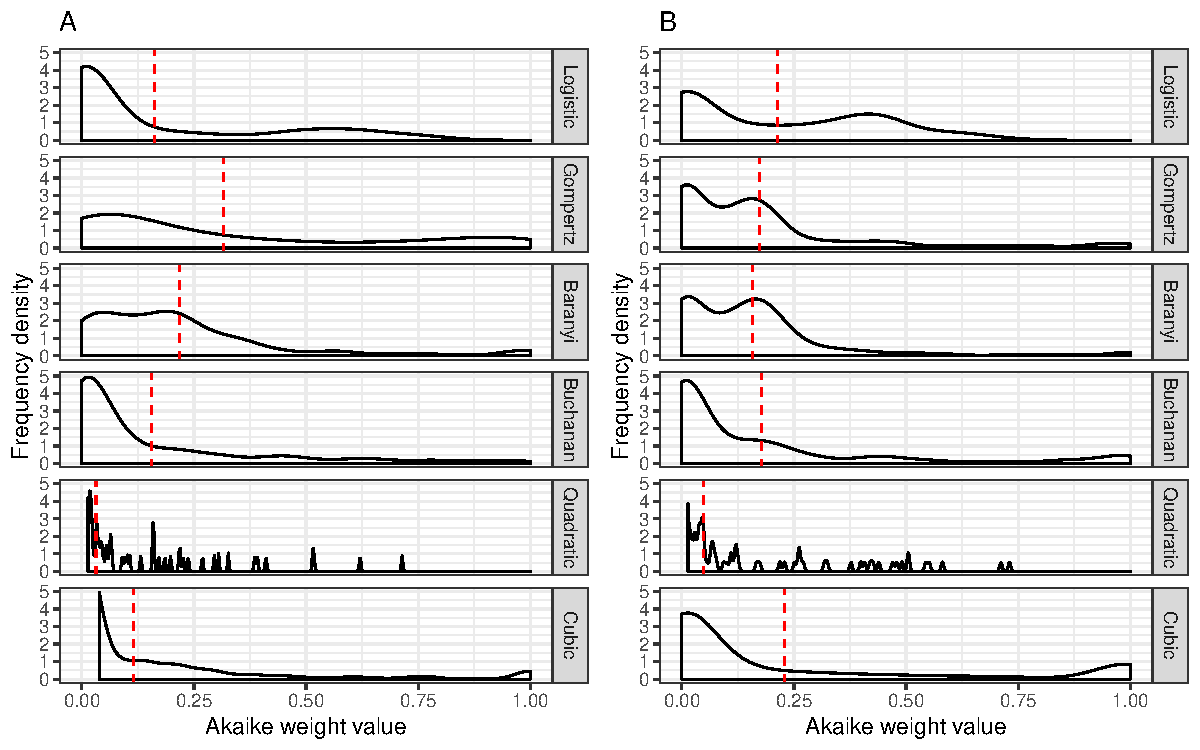
\includegraphics[height=3.5in]{../results/Aw_distributions.pdf}
        \caption{Gaussian Kernel Density Estimates for Akaike weights in logarithmic (A) and linear (B) space for each model. We see that in logarithmic space, the Gompertz model has strongest support, with the Logistic model have highly variable support due to its inability to model $t_{lag}$. In linear space, poor lag phase modelling is less strongly penalised, so the Logistic model gains the most support. }
        \label{fig:AWdist}
        \end{figure}
        
        

        
        \subsection{Logistic fit is poor when t\textsubscript{lag} is high}
                
        Notably, the Logistic model is the best model second most frequently despite its mean AIC and BIC scores placing fourth best - implying great variability in its performance. We can see this variability in its A\textsubscript{w} distribution, with high probability density near zero but a relative high density in the 0.5 to 0.75 interval (Figure \ref{AWdist}.  This can be explained by the absence of a lag phase in the model: the Logistic model fits poorly when a lag phase is present, but fits well when it is absent without incurring the AIC/BIC penalty for a fourth parameter. This is evident in the increasing proportion of points in the lag phase as the ranking of the logistic model gets worse (Figure \ref{fig:logistic_tlag} A). More explicitly, the difference in AIC between the Logistic and Gompertz model increases with proportion of data points in the lag phase (Figure \ref{fig:logistic_tlag} B). This relationship is strongly significant, with a linear regression estimating an increase in $\Delta_{\text{Logistic - Gompertz}}$ of 6.9 for every increase in lag phase proportion of 0.1, with a standard error of 0.47.
        
                \begin{figure}[H]
        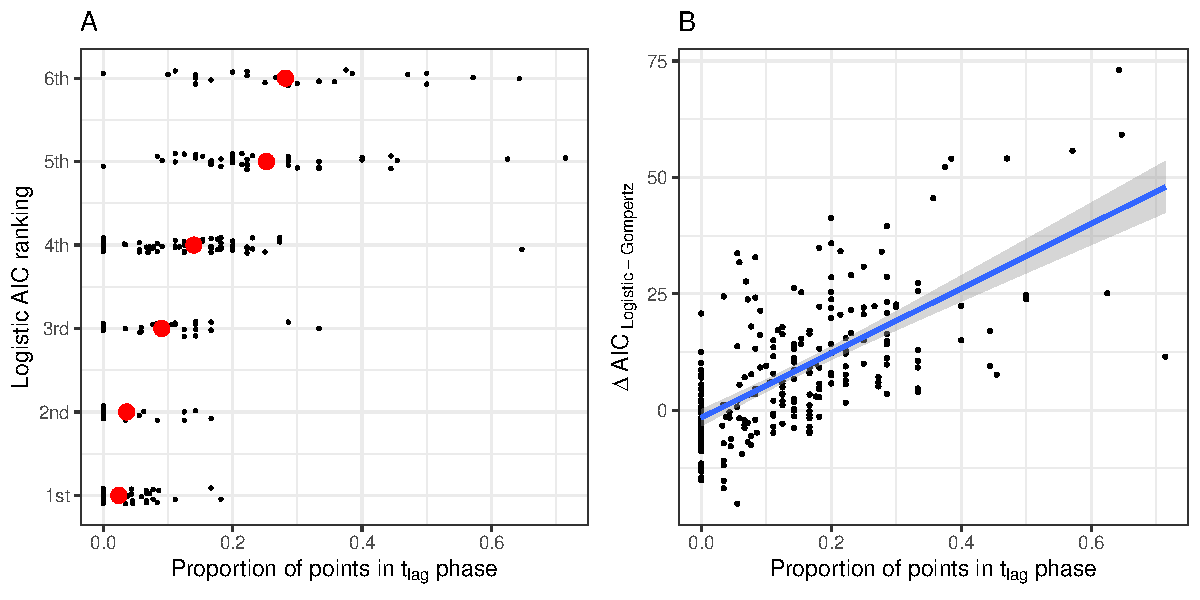
\includegraphics[width=\linewidth]{../results/tlag_vs_logistic.pdf}
        \caption{(A) is a plot of proportion of points in the lag phase, against the ranking of the Logistic model by AIC. We see that an increasing proportion of points in the lag phase is associated with a poorer ranking - with the mean proportion for each ranking shown by the red circle. (B) shows the difference in AIC score between the Gompertz and Logistic model against this proportion, with a statistically significant slope observed.}
        \label{fig:logistic_tlag}
        \end{figure}        
        
        \subsection{Temperature affects $\mu_{max}$ and $t_{lag}$}
        
         I ran a linear mixed model to determine the effect of temperature on $\mu_{max}$ and $t_{lag}$ across the entire data set, including species and medium as random effects. Temperature was included as a categorical variable as it is unlikely that the response to temperature is linear across the entire temperature range. From this, estimates for $\log(\mu_{max})$ and $t_{lag}$ values were be made for each temperature, shown in Figure \ref{fig:params_temp}. It is clear that the logarithm of the maximum rate of bacterial growth increases with temperature, approximately linearly across much of the temperature range, indicating an Arrhenius type thermal response. $t_{lag}$ decreases with temperature, quickly levelling off at around 10\degree C. 

         \begin{figure}[H]
        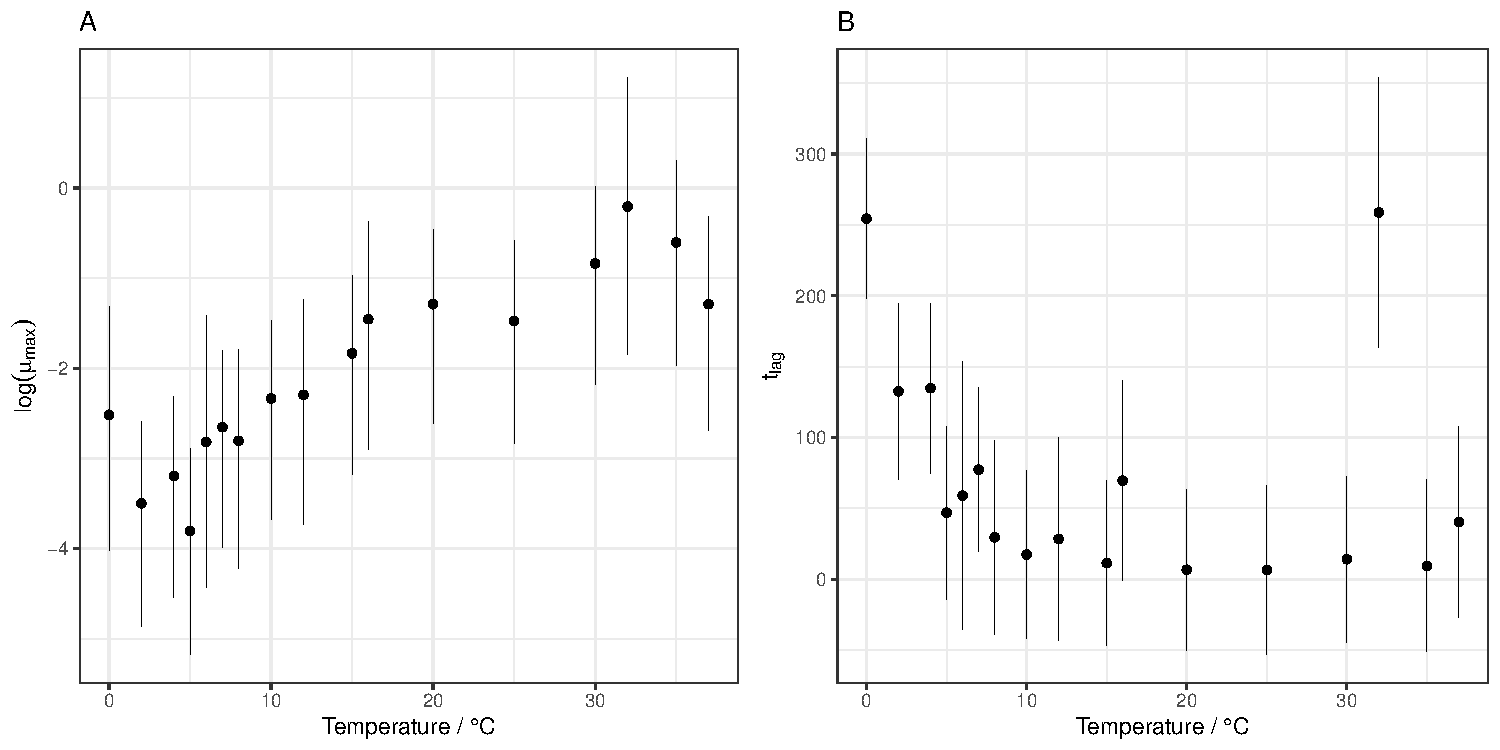
\includegraphics[width=\linewidth]{../results/tlags.pdf}
        \caption{(A) shows the relationship between $\mu_{max}$ and temperature, as estimated by a linear mixed model with temperature as a categorical variable. Vertical lines indicate the 95\% CI. $\mu_{max}$ increases steadily with temperature over the observed range. Similarly, (A) shows the relationship between $t_{lag}$ and temperature. We see that below 10\degree C, $t_{lag}$ increases rapidly as temperature decreases.   }
        \label{fig:params_temp}
        \end{figure}  



\subsection{Logistic model fits better at higher temperatures}

The decrease in $t_{lag}$ with temperature implies that the Logistic model, which has better fit with smaller $t_{lag}$, should have better fit with increasing temperature. Indeed, Figure \ref{fig:logistic_temp}A shows that $\Delta_{\text{Logistic - Gompertz}}$  decreases with increasing temperature. A linear regression suggests a decrease in $\Delta_{\text{Logistic - Gompertz}}$ of 3.30 for every 10\degree C, with standard error of 0.8.

        \begin{figure}[H]
        \centering
        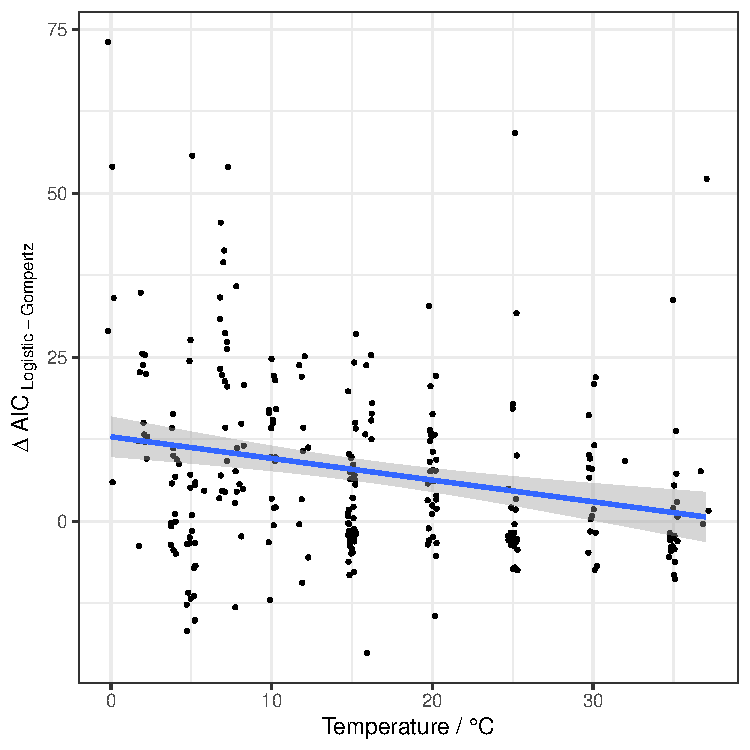
\includegraphics[width=4in]{../results/logistic_vs_gompertz_temp.pdf}
        \caption{$\Delta_{\text{Logistic - Gompertz}}$ is seen to decrease by 3.30 for every 10\degree C, indicating an improvement in the fit of the Logistic model relative to the Gompertz model as temperature increases.}
        \label{fig:logistic_temp}
        \end{figure}  

\subsection{Model choice biases parameter estimates}

Tables \ref{tab:tlag_biases} and \ref{tab:rmax_biases} show the mean pairwise differences in $t_{lag}$ and $\mu_{max}$ for the 4-parameter models. The Buchanan model results in the lowest $t_{lag}$ and lowest $\mu_{max}$ values. This is because the model assumes that population growth remains exactly at zero until $t = t_{lag}$, rather than smoothly transitioning to $\mu_{max}$ before this intercept. This means that Buchanan model fits must decrease $t_{lag}$ to capture the first part of the growth phase, consequently lowering $t_{lag}$ and $\mu_{max}$ values (Figure \ref{sup:fit_difference}).

\begin{table}[H]
\centering
\begin{tabular}{l|lll}
         & Gompertz                                        & Baranyi                                         & Buchanan                 \\ \hline
Gompertz & \cellcolor[HTML]{9B9B9B}                        & -5.21 = - 9.8\%                                           & 4.23 = 8.0\%                     \\
Baranyi  & \cellcolor[HTML]{9B9B9B}{\color[HTML]{9B9B9B} } & \cellcolor[HTML]{9B9B9B}{\color[HTML]{9B9B9B} } & 9.44 = 17.8\%                     \\
Buchanan & \cellcolor[HTML]{9B9B9B}{\color[HTML]{9B9B9B} } & \cellcolor[HTML]{9B9B9B}                        & \cellcolor[HTML]{9B9B9B}
\end{tabular}
\caption{Mean pairwise differences in $t_{lag}$ estimates for all models, and as proportions of the Akaike weighted mean $t_{lag}$ value. The value in $(i, j) = t_{lag}^i - t_{lag}^j$. The Buchanan model produces lower $t_{lag}$ estimates than either the Baranyi or the Gompertz models. All values are significant at the 5\% level.}
\label{tab:tlag_biases}
\end{table}


\begin{table}[H]
\centering
\begin{tabular}{l|lll}
         & Gompertz                                        & Baranyi                                         & Buchanan                 \\ \hline
Gompertz & \cellcolor[HTML]{9B9B9B}                        & -0.025 = -5.4\%                                           & 0.11 = 23.4\%                     \\
Baranyi  & \cellcolor[HTML]{9B9B9B}{\color[HTML]{9B9B9B} } & \cellcolor[HTML]{9B9B9B}{\color[HTML]{9B9B9B} } & 0.14 = 29.3\%                     \\
Buchanan & \cellcolor[HTML]{9B9B9B}{\color[HTML]{9B9B9B} } & \cellcolor[HTML]{9B9B9B}                        & \cellcolor[HTML]{9B9B9B}
\end{tabular}
\caption{Mean pairwise differences in $\mu_{max}$ estimates for all models, and as proportions of the Akaike weighted mean $t\mu{max}$ value. The value in $(i, j) = \mu_{max}^i - \mu_{max}^j$. The Buchanan model produces lower $\mu_{max}$ estimates than either the Baranyi or the Gompertz models. All values are significant at the 5\% level.}
\label{tab:rmax_biases}
\end{table}

\subsection{Model fitting in linear space fails to resolve the lag phase}
As discussed below, fitting the models to minimise linear RSS reduces the penalty for mischaracterising growth at small population sizes. The Logistic model is therefore favoured when fitting in linear space, despite its lack of a lag phase: it has the highest mean Akaike weight (Figure \ref{AWdist} B), is most frequently the best model, and has the lowest mean ranking (Figure \ref{sup:frequency_bar_linear} and Table \ref{suptable:meanAICBIClinear}). Further, the weakened penalisation of the lag phase means that the relationship between Logistic model fit and proportion of points in the lag phase is much weaker (Figure \ref{sup:logistic_temp_linear}), and the relationship with temperature becomes smaller and loses significance (Figure \ref{sup:logistic_temp_linear}). Finally, a paired t-test showed that fitting in linear space was associated with a reduction in the $t_{lag}$ parameter of 6.11 relative to logarithmic space, although with a 95\% CI extending from 0.53 to 11.70.



\section{Discussion}
\subsection{Mechanistic modelling is limited in its resolution between biological hypotheses}
The results are unequivocal about the importance of a lag phase for modelling microbial growth in logarithmic space, with the four-parameter models having the most support by Akaike weights, AICs, and BICs. Further, the fit of the Logistic model worsens with increasing lag phase duration. However, the difference in mean AIC between the Gompertz and Baranyi model is negligible, so no concrete mechanistic statements can be made - especially given that the Gompertz model is only mechanistic to the extent that it models the three canonical phases of the growth curve. Indeed, it has been argued that mechanistic modelling of this sort cannot strongly discern between biological hypotheses, which should be confirmed by direct observation or experimentation rather that argumentation about the cause of differences in model fit \cite{MicrobialGrowth}. Indeed, direct observation of the process of microbial growth can also provide us with estimates of parameters such as $t_{lag}$ and $\mu_{max}$ which currently have caveats in their interpretation, by directly counting and timing cell divisions. However, for parameter estimation and prediction in its current form, I propose that the Baranyi model is a stronger choice:

\begin{enumerate}
\item{Consistency: }
The Baranyi model is a more consistently good fit, achieving a marginally lower AIC despite rarely being the best fitting model. This implies that the Baranyi model can be deployed ore broadly and reliably than the Gompertz model, and that parameter estimates are likely to be more consistent.

\item{Truly mechanistic: }
The Baranyi model has the advantage that it was formulated entirely with microbial growth in mind, giving it a more mechanistic basis in microbial growth modelling, and therefore more interpretable parameters. The full Baranyi model also has extra curvature parameters $\nu$ and $m$, which alter the transition into and out of the exponential phase. As more data becomes available, these parameters can be estimated to form a more detailed understanding of the mechanisms behind microbial growth. Similarly, the Baranyi model's capacity to make predictions with non homogenous environmental conditions in its differential equation form makes it a much more flexible tool for growth modelling. 

 \end{enumerate}

\subsection{Lowering temperature can significantly impede microbial growth}

I find that $\log(\mu_{max})$ increases roughly linearly with temperature, corresponding to an exponential increase in $\mu_{max}$. Similarly, I find that $t_{lag}$ decreases rapidly with increasing temperature, such that the advantage of lower temperatures is almost entirely lost by 10 \degree C. Clearly, minimising the temperature of food storage can have a dramatic effect in decreasing microbial load - and conversely, increasing the temperature can result in growth orders of magnitude faster, with perhaps even brief exposure to higher temperatures able to spoil food. It will therefore be important to see how microbial growth patterns respond to temperatures that vary over time, which the Baranyi model will be very helpful in studying.

\subsection{Parameter biases necessitate caution in meta-analyses}

There is a clear hierarchy in the magnitude of parameter estimates from the three models. The Buchanan model produces the lowest $t_{lag}$ and $\mu_{max}$ estimates, with the Baranyi producing the highest, and Gompetz producing intermediate values. The magnitude of the differences between the Buchanan and Baranyi model reach 29\% of the Akaike weighted estimate for $\mu_{max}$, and 17\% for $t_{lag}$. These are extremely significant differences, so great care, probably involving reevaluation of raw data sets, is needed to ensure that parameter estimates from different sources are meaningfully compared, such that these biases are not interpreted as biological effects. A simulation study could be used to determine which model, or combination of models, produces the most reliable parameter estimate. Datasets produced by a variety of simulation mechanisms, with known 'true parameters' could be produced for a range of generative processes, and used to test how robust each of the models is to deviations from their mechanistic assumptions, and to noise in the data.

\subsection{Fitting in logarithmic space is required to estimate relevant parameters}
When fitting in linear space, the logistic model is most supported. This is a strong remit to recommend that logarithmic space should be used, as the success of the Logistic model demonstrates that linear space fitting only weakly enforces accurate modelling of the lag phase. As linear space fitting is concerned with modelling absolute, rather than relative, population size, mischaracterisation of the early growth phase is not strongly penalised. The ability to describe the lag phase as the early stage of population growth also leads to systematically lower $t_{lag}$ estimates when fitting in linear space. Fitting in logarithmic space is therefore strongly recommended for food preservation work, where early growth curve behaviour is of centrally interest as food is often spoiled before $N_{max}$ is reached \cite{MicrobialGrowth}.

As such, this study has demonstrated that the choice of space and model in microbial growth modelling can have profound effects both on parameter estimates, and may even even conceal findings. Further work examining the reliability of the various models to violations of their assumptions is needed to devise strategies that can provide the most accurate parameter estimates, which will allow increasingly quantitative approaches to food preservation.


\end{linenumbers}

\section{Supplementary Material}
\beginsupplement

        \begin{figure}[H]
        \includegraphics[width=\linewidth]{../results/compare_log_lin_fit.pdf}
        \captionsetup{format=hang}
        \caption{Comparison of: (A) fitting and evaluating modelling in log space. (B) fitting model in log space, evaluating fit in linear space. (C) fitting and evaluating model in linear space. \newline When the models are fit and evaluated in log space, it is clear that the Gompertz model has a better fit. However, if evaluation is done in linear space of these fits, the logistic model appears to have a better fit. This is shown to be invalid, as fitting the models in linear space demonstrates that the Gompertz model can in fact achieve better fits in both spaces.  }
        \label{sup:compare_least_squares}
        \end{figure}
        
        
        \begin{figure}[H]
        \centering
        \includegraphics[width=3.5in]{../results/rolling_reg.pdf}
        \caption{Rolling regression was used to produce starting parameters. The regression line with the greatest gradient was selected, with its gradient used as $\mu_{max}$, and its intercept with $N = \min(N)$ used as $t_{lag}$ }
        \label{sup:rolling_regression}
        \end{figure}  
        
        
         \begin{figure}[H]
        \includegraphics[width=\linewidth]{../results/removed_ids.pdf}
        \caption{The 64 datasets with the lowest maximum R\textsuperscript{2}. Those which were manually removed are highlighted with a red border.}
        \label{sup:removed_ids}
        \end{figure}
        
         \begin{figure}[H]
        \includegraphics[width=3.5in]{../results/constraint_demo.pdf}
        \centering
        \caption{If there are too few points in the growth phase, $\mu_{max}$ and $t{lag}$ will not be well constrained. Here, we can see that there are infinitely many solutions that can fit equally well to the data as there is only one point in the growth phase. }
        \label{sup:constraint}
        \end{figure}  


         \begin{figure}[H]
         \centering
        \includegraphics[height=4.5in]{../results/model_fits_linear.pdf}
        \caption{Demonstration of model fits in linear space. Out of 287 data sets, all fits were successful apart from a single fit of the Buchanan model, to a dataset which was removed anyway.}
        \label{sup:model_fits_linear}
        \end{figure}

         \begin{figure}[H]
        \includegraphics[width=4in]{../results/fit_difference.pdf}
        \centering
        \caption{The Buchanan and Gompertz models are fit to the same hypothetical growth data, which results in smaller $t_{lag}$ and $\mu_{max}$ estimates from the Buchanan model in order to capture the start of the growth phase. By contrast, there is some growth before $t = t_{lag}$ in the Gompertz model.}
        \label{sup:fit_difference}
        \end{figure} 
        
        
         \begin{figure}[H]
        \includegraphics[width=4in]{../results/best_fit_frequency_bar_linear.pdf}
        \centering
        \caption{Plots showing rankings of models in linear space. (A) shows the number of times each model is the best fitting model for a dataset. (B) shows the number of times each model is the second best fitting model for a dataset. (C) shows the mean ranking for each model. (D) shows the number of times each model is the best fitting model for a dataset if we do not consider the Gompertz and Buchanan models.  In linear space, the logistic model performs better than it does in log space, as less emphasis is put on the lag phase.}
        \label{sup:frequency_bar_linear}
        \end{figure} 
        
\begin{table}[H]
\centering
\begin{tabular}{l|llllll}
       & Logistic & Gompertz & Baranyi & Buchanan & Quadratic & Cubic \\ \hline
AIC & 62.3    & 61.8    & 61.3   & 65.5    & 76.3     & 67.7 \\
BIC & 63.8    & 63.8    & 63.3   & 67.5    & 77.8     & 69.7 \\
$A_w$ & 0.213     & 0.174    & 0.158   & 0.178     & 0.0493     &   0.229

\end{tabular}
\caption{Mean AIC, BIC, and Akaike weight values for each model fitted in linear space}
\label{suptable:meanAICBIClinear}
\end{table}




        
        \begin{figure}[H]
        \includegraphics[width=5in]{../results/tlag_vs_logistic_linear.pdf}
        \centering
        \caption{(A) is a plot of proportion of points in the lag phase, against the ranking of the Logistic model by AIC in linear space. (B) shows the difference in AIC score between the Gompertz and Logistic model against this proportion, In both cases, the relationship between Logistic model performance and $t_{lag}$ is much weaker than in log space. The difference in AIC between Logistic and Gompertz decreases by 2.4 for every increase in lag phase proportion by 0.1 (in contrast to 6.9 for log space)}
        \label{sup:tlag_logistic_linear}
        \end{figure} 
        
         \begin{figure}[H]
        \includegraphics[width=3in]{../results/logistic_vs_gompertz_temp_linear.pdf}
        \centering
        \caption{$\Delta_{\text{Logistic - Gompertz}}$ no longer has a statistically significant relationship with temperature when models are fit in linear space. This implies that the fit of the Logistic model does not become any weaker realtive to thegompertz model as temperature increases.}
        \label{sup:logistic_temp_linear}
        \end{figure} 
        
        \begin{figure}[H]
        \includegraphics[width=\linewidth]{../results/tlags_linear.pdf}
        \centering
        \caption{The broad patterns of $\mu_{max}$ and $t_{lag}$ are the same when model fitting is in linear space, but the confidence intervals are much broader.}
        \label{sup:params_linear}
        \end{figure} 
        
        
    \bibliographystyle{ieeetr}
    \bibliography{write_up}

\end{document}
}

\newcommand{\beginsupplement}{%
        \setcounter{table}{0}
        \renewcommand{\thetable}{S\arabic{table}}%
        \setcounter{figure}{0}
        \renewcommand{\thefigure}{S\arabic{figure}}%
     }







\begin{document}

    \begin{titlepage}
	\centering
	\includegraphics[width=0.5\textwidth]{../data/imperial.png}\par\vspace{1cm}
	\vspace{2cm}
	{\scshape\Large\bfseries Comparison of Methodologies to Fit Microbial Population Growth Models\par}
	\vspace{2cm}
	{\Large Sam Turner\par}
	\vspace{0.5cm}
	{\Large March 2020 \par}
	\vspace{0.5cm}
	{\Large\itshape Computational Method in Ecology and Evolution MSc\par}
	\vspace{0.5cm}
	 \wordcount words 
	\vfill

	\vfill
    
    \newpage
    \end{titlepage}
    
    \begin{abstract}
    The modelling of microbial growth is vital for developing food preservation measures to decrease food waste. By fitting a range of mechanistic and phenomenological models to a large dataset of 305 growth curves, I demonstrate that temperature has a major impact on microbial population dynamics. I also show that model fitting in log space increases the resolution of parameter estimates relative to linear space model fitting, and that different models with equivalent parameterisations can produce systematically biased parameter estimates. This results in recommendations for model fitting, and in particular how to carry out meta analyses where parameter values must be compared between sources.
\end{abstract}

\begin{linenumbers}
    \section{Introduction}
    
    There is great interest in modelling the growth of microbial populations, such that the biology of microbial growth and its response to external variables can be understood \cite{zwitmodelling}. Through this modelling, food shelf life can be predicted, and preservation methods can be optimised. In this project, I aim to answer four questions:    
      


\begin{enumerate}
  \item Which models best describe microbial population growth, and how does this vary with temperature?
  \item How does choice of model affects parameter estimates?
  \item What are the qualitative patterns of how temperature affects microbial growth?
  \item Does the choice to fit models in linear or log space affect results?
  \end{enumerate}


I aimed to answer these questions by fitting a range of mechanistic and phenomenological models to a large dataset of 305 digitised growth curves. The mechanistic models each attempt to describe the shape of the bacterial growth curve with a mathematical relationship representing a real hypothesis about the dynamics of the microbial population \cite{Buchanan}, and therefore can be parameterised with meaningful biological quantities. This is in contrast to the phenomenological models, which are simply mathematical functions that we attempt to fit to the data, and can be used as a neutral comparison for the mechanistic models. By comparing the fit of the mechanistic models to each other, and to the phenomenological models, we can determine which underlying biological hypothesis has the best support from the data - and how this support varies with temperature.

I also examine how temperature affects the growth rate and lag time of bacterial populations, the dynamics of which play a central role in food spoilage. It is also important to determine whether the parameter estimates from various mechanistic models with analogous parameterisations vary significantly, as this may invalidate comparison of parameter values from different sources in meta-analyses.

\subsection*{The Mechanistic Models}

The mechanistic models can be split into three four-parameter models, and the three-parameter logistic model. The four-parameter models split the bacterial growth curve into a lag phase, exponential growth phase, and stationary phase, with the three-parameter logistic model discarding the lag phase.

\paragraph*{Logistic}
The logistic model \cite{logisticVel1, logisticVel2} assumes that the microbial population immediately starts growing exponentially, with its growth rate falling towards zero as the population size approaches a carrying capacity. This is described by the logistic differential equation:

\[ \frac{\mathrm d N}{\mathrm d x} =  \mu_{max}N(1-N)  \]

Which has solutions:

\[ N_t =   \frac{N_0  N_{max} e^{\mu t}}{N_{max} + N_0 (e^{\mu t} - 1)} \]


\subsubsection{Four-parameter models}

The four-parameter models parameterise the sigmoidal growth curve with minimum and maximum population sizes, maximum growth rate, and a time lag before the population starts growing - defined as the intercept between the tangent to the curve at the point of inflection, and the line $N = N_0$ (Figure \ref{fig:parameter_variation_demo} ). As such, the rate of growth and length of the lag phase can be independently varied (Figure \ref{fig:4_param_demo} )

        \begin{figure}[H]
        \centering
        \includegraphics[width=4in]{../results/4_param_demo.pdf}
        \caption{Illustation of $\mu_{max}$ and $t_{lag}$ parameters. $\mu_{max}$ is the maximum gradient of the growth curve, and $t_{lag}$ is the intercept between this tangent line and the line $N = N_0$}
        \label{fig:4_param_demo}
        \end{figure}


        \begin{figure}[H]
        \includegraphics[width=\linewidth]{../results/tlag_rmax_demo.pdf}
        \caption{ $\mu_{max}$ (A) and $t_{lag}$ (B) parameters can be varied independently to control the rate of microbial growth, and the duration of the lag phase.}
        \label{fig:parameter_variation_demo}
        \end{figure}



\paragraph*{Buchanan}
The Buchanan model \cite{Buchanan} is the simplest implementation of this, assuming that the population has a growth rate of zero during the lag and stationary phases, with a period of exponential growth at a constant rate between this:

  \[
    log(N_t) = \begin{cases}{}
        N_0 & \quad \text{if } t\leq t_{lag}\\
        N_0 + \mu_{max} \cdot (t - t_{lag}) &  \quad \text{if } t_{lag}\leq t\leq t_{max}\\
        N_{max} &  \quad \text{if } t\geq t_{max}
        \end{cases}
  \]

\paragraph*{Gompertz}

The Gompertz model\cite{Gomp, zwitmodelling} similarly describes a sigmoidal growth curve, adding a gradual transition into and out of the exponential phase. The Gompertz model has long been popular for microbial population modelling, as it has empirically been found to fit well in a wide range of circumstances. However, it should be noted that its derivation does not have a mechanistic basis in population growth modelling \cite{EstBaranyi}, but rather in describing human mortality rates \cite{Gomp}. 

  \[log_{10}(N_t) = N_0 + (N_{max} - N_0)  e^{-e^{ \frac{\mu_{max} ~ \cdot ~ e  ~ \cdot ~ (t_{lag} - t)}{ (N_{max} - N_0) ~ \cdot ~ log(10)} + 1} }\]
  
  
\paragraph*{Baranyi}

The Baranyi model is an attempt to formulate a truly mechanistic model for microbial population growth \cite{BaranyiOriginal,, zwitmodelling}, explicitly modelling the internal physiological state and external environmental conditions of the cell. This mechanistic formulation produces a much more flexible and widely applicable model, which can be applied to model population growth curves in time-varying environmental conditions. Here,  we use a version of the model in which conditions are homogenous, with the curvature parameter into the exponential phase $\nu$ set to $\mu_{max}$, and curvature parameter out of the exponential phase $m$ set at an empirical estimate of 1:

\[ log_{10}(N_t) = N_{max} + log_{10}(\frac{-1 + e^{\mu_{max} \cdot  t} + e^{\mu_{max} \cdot t_{lag}  } }{ -1 + e^{\mu_{max} \cdot t}  + e^{\mu_{max} \cdot t_{lag}} \cdot 10^{N_{max}-N_0}}) \]


        \begin{figure}[h]
        \includegraphics[width=\linewidth]{../results/model_demo.pdf}
        \captionsetup{format=hang}
        \caption{Demonstration of the shape of the 4 mechanistic models, plotted in log space. The logistic model (A) immediately starts growing at its maximum growth rate, whilst the three four-parameter models (B) have growth phases that transition into the exponential phase}
        \label{fig:models_demo}
        \end{figure}

\subsection*{Phenomenological models}
As controls, I decided to fit quadratic and cubic polynomials to the data:
\paragraph*{Quadratic} $ N_t = at^2 + bt + c $
\paragraph*{Cubic} \quad \quad $ N_t = at^3 + bt^2 + ct + d $


   \section{Methods}
   
   \subsection{Data}
   
\paragraph{Data sources}
The provided microbial growth data contained 305 population size time series, digitised from graphs in 10 papers from the microbial growth literature. The data set contained time series from 47 different species, 18 media, and 17 temperatures, with population size measured in 4 different units. However, the data from one citation \cite{discarded} clearly had incorrect time values, with times extending to 13,000 hours. I removed the data from this citation as there was not a clear correct transformation to produce the correct times, with time values appeared to be have multiplied by around 20 relative to the original paper. This left 287 time series for analysis.

\paragraph{Log transformation}
As explained below, I decided to fit the model to $log_{10}(N)$ as well as to linear data. In 5 /287 data sets, there were negative population counts due to numerical error in growth curve digitization. One value of approximately -668, which was removed, whilst other values were greater that -10\textsuperscript{-2} - in these cases, I transformed increased population sizes for that time series by the minimum population size in the time series, discarding the minimum value of 0 before taking the logarithm.  

\paragraph{Time transformation}
I transformed each time series such that the first data point was at $t = 0$ for fitting the four-parameter models, as model fits were clearly suboptimal without this transformation. Since $t_{lag}$ directly transforms the curve along the t-axis, $t_{lag}$ could be adjusted back to obtain model parameters which fit the untransformed time series. 

\subsection{Model Fitting}
When fitting the models, I used a least squares approach, both to log\textsubscript{10} transformed data, and to the original linear data (Figure \ref{compare_least_squares}. This required reformulating the four-parameter models to predict linear population size, by exponentiating the right hand side of the function, and reformulating the logistic model to predict log population size, by taking the logarithm of the right hand side. As such, the parameters of the four-parameter models remained in log space, and the parameters of the Logistic model in linear space. 

Principally, the difference between fitting in linear space and log space is whether we are concerned with absolute values or relative values. Log space expands variation at small population sizes, and therefore more strongly highlights the lag phase. This makes estimation of t\textsubscript{lag} more robust, and means that models such as the logistic model are more strongly penalised for mischaracterising small population sizes early in the time series due to the absence of a lag phase. By contrast, in linear space model fit is strongly weighted towards large absolute population sizes. For food preservation purposes, this is undesirable, as the the lag phase is more interesting than behaviour near N\textsubscript{max}, as food is often spoiled long before this.  

As such, I decided to use parameter estimates from the log-fitted models for my main analysis (although linear fit results are presented in the Supplementary Figures), also choosing not to linearise residuals, as this resulted in non-sensical fits (demonstrated in Figure \ref{sup:compare_least_squares}). These fits can be explained by the fact that, in general:
\[log(f(x) ) \neq f(log(x))\]
This means that minimising errors in log space does not result in minimised errors in linear space, so evaluating fit in linear space would not capture the best possible fit for each model, (Figure \ref{sup:compare_least_squares}).

\subsubsection{Fitting linear models}

The two polynomial phenomenological models are linear in their parameters, so were fitted using Ordinary Least Squares with the lm() function in R \cite{R}.

\subsubsection{Fitting non-linear models}

The mechanistic models are non-linear, so most be fitted using an optimisation approach. The nlsLM function in the minpack.lm \cite{minpack} package uses the Levenberg-Marquardt algorithm to find parameter values for a specified model.  The optimiser requires initial values for the parameters, which are optimised to minimise RSS. If these initial values are far from the true optimal parameters, it is likely that the optimisation will not converge, or will converge to very suboptimal parameters. It is therefore important to  estimate reasonable starting values to provide to the optimiser.

\paragraph{Estimating parameter values}
For the logistic model, parameters are in linear space (even though RSS is minimised in log space), whereas for the four-parameter models, the parameters are in linear space. Therefore, the following parameter estimation method was carried out both on population size and log population size. 

N\textsubscript{min} and N\textsubscript{max} were set as the minimum and maximum observed population size respectively. $\mu_{max}$ and $t_{lag}$ estimates were determined using a rolling regression (Figure \ref{sup:rolling_regression}), which computed the regression line for every possible set of 5 adjacent data points. The regression line with the greatest gradient was selected, with the gradient taken as an estimate of $\mu_{max}$, and the $t$ value of the intercept between this selected regression line with the line $N = \min(N)$ taken as the $t_{lag}$ estimate . 


     

\paragraph{Multiple fit attempts}
Even with reasonably chosen parameter estimates, models often fail to converge, or converge to poorly fitting parameter values. In order to increase the proportion of models which fit, and to ensure that parameter values nearer the global optimum were found, I used a grid search to test a range of initial parameter values. I specified a range for each parameter in each model surrounding the estimated parameter value. For each parameter, I choose linearly spaced samples from this range, and tested every possible combination of these parameter values. For example, if I take 3 linearly spaced samples for each of $N_0$ and $N_{max}$, and 5 for $t_{lag}$ and $\mu_{max}$, I fit $3 \times 3 \times 5 \times 5 = 225$ models. From the model fits that converge, I select the model with the smallest RSS. If none of the models converge, I randomly sample parameter values with normally distributed noise around my parameter estimates until a model fits, or until there have been 1,000 failed attempts. 

Using this method, I was able to fit all 287 data sets for the Logistic, Gompertz, and Baranyi models in both linear space and log space. In linear space, there was one failed fit for the Buchanan model, and in log space there were two failed fits for the Buchanan model.


\subsection{Filtering}
Some data sets show no pattern of population growth, or have too few points in the growth phase to constrain the $mu_{max}$ and $t_{lag}$ parameters. The 64 data sets with the lowest maximum R\textsuperscript{2} value were visualised, of which 20 with no meaningful growth pattern were removed (Figure \ref{sup:removed_ids}). For analyses involving parameter estimates, I further filtered out datasets with less than 2 points in the growth phase (Figure \ref{sup:constraint}).  This involved counting the number of points that have a time value within the predicted exponential phase. The predicted exponential phase was determined using Akaike weighted parameter values. This removed a further 57 data sets, leaving 210 data sets for parameter estimate analysis.


\subsection{Model Selection}

Model fit was assessed using AIC \cite{AIC} and BIC \cite{BIC}. With the assumption of normally distributed errors, and simplification to remove constants, these are:
\[\text {AIC}  = 2k + n\log(RSS)\]
\[\text {BIC} = n\log{\frac{RSS}{n}} + k\log{n}\]

As these are dependent on the number of parameters of the model, they can be used for direct comparison of fit for models with differing numbers of parameters. For each data set, the model with the lowest AIC/BIC value was selected as the best fit model.


\subsection{Parameter Estimation}

Parameter estimation was performed using Akaike weights, which produce a single parameter estimate from a family of models \cite{ModelSelection}, weighted by the model’s $\Delta_{AIC}$ value:
With $\text{AIC}_{best}$ being the lowest observed AIC values for a dataset, $\Delta_{AIC}$ values are calculated with:
\[ \Delta_i = \text{AIC}_i - \text{AIC}_{best} \]

The Akaike weight for the $i^{th}$ model is then:
\[ w_i = \frac{e^{-\frac{1}{2}\Delta_i }} { \sum_{r = 1}^{r = R}  e^{- \frac{1}{2}\Delta_r }}\]

The Akaike weighted parameter estimate for $\theta$, with weights $w_i$ and individual model parameter estimates $\theta_i$ is:
\[\theta_w = \sum_{i = 1}^{i = I}\theta_i * w_i\]


\subsection{Statistical Analysis}

I ran linear regressions of $\Delta_{\text{Logistic - Gompertz}}$ against temperature, and $\Delta_{\text{Logistic - Gompertz}}$ against proportion of points in the lag phase. These were carried out using lm() in R \cite{R}, with their diagnostic plots examined to confirm the suitability of a linear model.

I ran a mixed effects model of $\mu{max}$ against temperature, and of $t_{lag}$ against temperature, with species and medium used as random effects in each case. Again, diagnostic plots were used to confirm that residuals were homogeneous across the fitted values.

I ran a paired t-test between the each pair of the four-parameter models to check for systematic differences in their parameter estimates. I check for normality of differences by plotting histograms of these differences.  

\subsection{Computing Tools}
\subsubsection{R 3.6.1 \cite{R}} Used for initial data preparation script, for model fitting, for analysis, and for figure preparation. I chose R for these tasks because the native data structures are natural tools for handling this type of data. The native support of vectorised operations also makes the code cleaner than it would be in Python. I chose to write my multi-start method to fit models over a range of initial parameter values in R because of the robustness and efficiency of non-linear least squares model fitting in the minpack.lm package.
\begin{itemize}
\item \textbf{minpack.lm \cite{minpack}:} Non-linear least squares model fitting using the more robust Levenberg-Marquardt algorithm.
\item \textbf{ggplot2 \cite{gg}:} To more easily create high quality graphics.
\item \textbf{dplyr \cite{dplyr}:} For some data wrangling tasks.
\item \textbf{lme4 \cite{lme4}:} For fitting linear mixed models.
\item \textbf{toOrdinal \cite{tO}:} For creating ordinal numbers for annotation.
\end{itemize}

\paragraph{Python 3.7.4 \cite{python}} Used for calculation of initial values.
\begin{itemize}
\item \textbf{pandas \cite{pd}:} For dataframes in python
\item \textbf{matplotlib \cite{plt}:} To create graphics in python
\item \textbf{scipy \cite{numpy}:} For linear model fitting in python
\item \textbf{numpy \cite{numpy}:} For efficient arrays in python
\end{itemize}

\LaTeX Used for compilation of write up.
\section{Results}

\subsection{Model fitting is highly successful}
The method of taking the best fitting model from a range of initial parameter values was very effective, with all models converging to every time series when those with no discernible growth pattern were removed, and only 3 unsuccessful fits otherwise (2293 / 2296 successful fits overall). The model fits were visually inspected, and found to describe the data well (Figure \ref{fig:model_fits} for log space fits, Figure \ref{sup:model_fits_linear} for linear space fits). For the reasons mentioned in the Model fitting section of Methods, I discuss the results obtained from fitting models in log space first, before presenting the results from linear space fits at the end of this section.

                \begin{figure}[H]
                \centering
        \includegraphics[height=4.5in]{../results/model_fits.pdf}
        \caption{Demonstration of model fits in log space. Out of 287 data sets, all fits were successful apart from two fits of the Buchanan model, to datasets which were removed anyway. }
        \label{fig:model_fits}
        \end{figure}

\subsection{Gompertz and Baranyi are best supported}

I found that the model which most frequently had the lowest AIC and BIC values was the Gompertz model, which was determined to be the best fit model in 91 of 267 cases with AIC, and 90 cases with BIC (Figure \ref{fig:bestbars} A). Although second most frequent best model is the Logistic model, this should not be interpreted as the Logistic model having the second most support from the data. From the means and distributions of AIC values (Figure \ref{fig:AICBICdist} and Table \ref{table:meanAICBIC}), we can see that the Baranyi model in fact has a slightly lower mean AIC score and slightly lower mean ranking than even the Gompertz model (Figure \ref{fig:bestbars} B and C), despite being the best fit model on only 35 occasions. This can be explained by the fact that the Baranyi model is  often the second best fitting model - on 131 out of 267 occasions, in fact. It therefore must be common that the Gompertz model is the best fitting model with the Baranyi model just behind in second, with many cases of the Baranyi model being first or second with the Gompertz performing much more poorly, such that its AIC and BIC become slightly worse than the Baranyi model's. Indeed, when we include the Baranyi model as the only 4 parameter model, it is the best fitting model on 130 occasions (Figure \ref{fig:bestbars} D)




        \begin{figure}[H]
        \includegraphics[width=\linewidth]{../results/best_fit_frequency_bar.pdf}
        \caption{Plots showing the rankings of models in log space. (A) shows the number of times each model is the best fitting model for a dataset. (B) shows the number of times each model is the second best fitting model for a dataset. (C) shows the mean ranking for each model. (D) shows the number of times each model is the best fitting model for a dataset if we do not consider the Gompertz and Buchanan models. }
        \label{fig:bestbars}
        \end{figure}
        
         \begin{table}[H]
\centering
\begin{tabular}{l|llllll}
       & Logistic & Gompertz & Baranyi & Buchanan & Quadratic & Cubic \\ \hline
AIC & -58.5    & -66.2    & -66.3   & -61.1    & -43.7     & -53.2 \\
BIC & -57.0    & -64.1    & -64.2   & -59.1    & -42.2     & -51.1
\end{tabular}
\caption{Mean AIC / BIC values for each model, fitted in log space.}
\label{table:meanAICBIC}
\end{table}


        \begin{figure}[H]
        \includegraphics[height=3.5in]{../results/AIC_BIC_distributions.pdf}
        \caption{Gaussian Kernel Density Estimates for AIC (A) and BIC (B) distributions for each model. We can see that the choice of AIC or BIC makes little difference.}
        \label{fig:AICBICdist}
        \end{figure}
        
        

        
        \subsection{Logistic fit is poor when t\textsubscript{lag} is high}
        
        It is notable that the Logistic model is the best model second most frequently, but that its mean AIC and BIC scores are only fourth best overall - which implies great variability in its performance. This can be explained by the absence of a lag phase in the model: when the data exhibits a lag phase, the Logistic model fits poorly, but when there is no lag phase, it is able to fit the data well without incurring the AIC/BIC penalty for a fourth parameter. This is evident in the increasing proportion of points in the lag phase as the ranking of the logistic model gets worse (Figure \ref{fig:logistic_tlag} A). More explicitly, we can see that the difference in AIC between the Logistic and Gompertz model increases with proportion of data points in the lag phase (Figure \ref{fig:logistic_tlag} B), indicating that the Gompertz model has an increasing advantage over the Logistic model as the lag phase increases in duration. This relationship is strongly significant, with a linear regression of $\Delta_{\text{Logistic - Gompertz}}$ against proportion of lag phase points produces an estimated increase in $\Delta_{\text{Logistic - Gompertz}}$ of 6.5 for every increase in lag phase proportion of 0.1, with a standard error of 0.49.
        
                \begin{figure}[H]
        \includegraphics[width=\linewidth]{../results/tlag_vs_logistic.pdf}
        \caption{(A) is a plot of proportion of points in the lag phase, against the ranking of the Logistic model by AIC. We see that an increasing proportion of points in the lag phase is associated with a poorer ranking - with the mean proportion for each ranking shown by the red circle. (B) shows the difference in AIC score between the Gompertz and Logistic model against this proportion, with a statistically significant slope observed.}
        \label{fig:logistic_tlag}
        \end{figure}        
        
        \subsection{Temperature affects $\mu_{max}$ and $t_{lag}$}
        
         I ran a linear mixed model to determine the effect of temperature on the $\mu_{max}$ and $t_{lag}$ parameters across the entire data set. Each of these models included species and medium as random effects, and temperature included as a categorical variable as it is unlikely that the response to temperature is linear across the entire temperature range. From this, estimates for $\log(\mu_{max})$ and $t_{lag}$ values could be made for each temperature, which are shown in Figure \ref{fig:params_temp}. It is clear that the log of the maximum rate of bacterial growth increases with temperature, approximately linearly across much of the temperature range, indicating an Arrhenius type functional response. $t_{lag}$ decreases with temperature, quickly levelling off at around 10\degree C. 

                \begin{figure}[H]
        \includegraphics[width=\linewidth]{../results/tlags.pdf}
        \caption{(A) shows the relationship between $\mu_{max}$ and temperature, as estimated by a linear mixed model with temperature as a categorical variable. Vertical lines indicate the 95\% CI. $\mu_{max}$ increases steadily with temperature over the observed range. Similarly, (A) shows the relationship between $t_{lag}$ and temperature. We see that below 10\degree C, $t_{lag}$ increases rapidly as temperature decreases.   }
        \label{fig:params_temp}
        \end{figure}  



\subsection{Logistic model fits better at higher temperatures}

The decrease in $t_{lag}$ with temperature implies that the Logistic model, which has better fit with smaller $t_{lag}$, should have better fit with increasing temperature. Indeed, we can see that this is the case in Figure \ref{fig:logistic_temp} A, which shows that $\Delta_{\text{Logistic - Gompertz}}$  decreases with increasing temperature - implying that the Logistic model gets better support relative to the Gompertz model at higher temperatures. A linear regression suggests a decrease in $\Delta_{\text{Logistic - Gompertz}}$ of 3.30 for every 10\degree C, with standard error of 0.8.

                \begin{figure}[H]
                \centering
        \includegraphics[width=4in]{../results/logistic_vs_gompertz_temp.pdf}
        \caption{$\Delta_{\text{Logistic - Gompertz}}$ is seen to decrease by 3.30 for every 10\degree C, indicating an improvement in the fit of the Logistic model relative to the Gompertz model as temperature increases.}
        \label{fig:logistic_temp}
        \end{figure}  

\subsection{Model choice biases parameter estimates}

Tables \ref{tab:tlag_biases} and \ref{tab:rmax_biases} show the mean pairwise differences in $t_{lag}$ and $\mu_{max}$ for the 4-parameter models. We can see that the Buchanan model results in the lowest $t_{lag}$ and lowest $\mu_{max}$ values. This can be explained by the fact that the model assumes that the population growth remains exactly at zero until $t = t_{lag}$, rather than smoothly transitioning to $\mu_{max}$ before this intercept. This means that Buchanan model fits must decrease $t_{lag}$ to capture the first part of the growth phase, consequently lowering $t_{lag}$ and $\mu_{max}$ values (Figure \ref{sup:fit_difference}).

\begin{table}[H]
\centering
\begin{tabular}{l|lll}
         & Gompertz                                        & Baranyi                                         & Buchanan                 \\ \hline
Gompertz & \cellcolor[HTML]{9B9B9B}                        & -5.21 = - 9.8\%                                           & 4.23 = 8.0\%                     \\
Baranyi  & \cellcolor[HTML]{9B9B9B}{\color[HTML]{9B9B9B} } & \cellcolor[HTML]{9B9B9B}{\color[HTML]{9B9B9B} } & 9.44 = 17.8\%                     \\
Buchanan & \cellcolor[HTML]{9B9B9B}{\color[HTML]{9B9B9B} } & \cellcolor[HTML]{9B9B9B}                        & \cellcolor[HTML]{9B9B9B}
\end{tabular}
\caption{Mean pairwise differences in $t_{lag}$ estimates for all models, and as proportions of the Akaike weighted mean $t_{lag}$ value. The value in $(i, j) = t_{lag}^i - t_{lag}^j$. The Buchanan model produces lower $t_{lag}$ estimates than either the Baranyi or the Gompertz models. All values are significant at the 5\% level.}
\label{tab:tlag_biases}
\end{table}


\begin{table}[H]
\centering
\begin{tabular}{l|lll}
         & Gompertz                                        & Baranyi                                         & Buchanan                 \\ \hline
Gompertz & \cellcolor[HTML]{9B9B9B}                        & -0.025 = -5.4\%                                           & 0.11 = 23.4\%                     \\
Baranyi  & \cellcolor[HTML]{9B9B9B}{\color[HTML]{9B9B9B} } & \cellcolor[HTML]{9B9B9B}{\color[HTML]{9B9B9B} } & 0.14 = 29.3\%                     \\
Buchanan & \cellcolor[HTML]{9B9B9B}{\color[HTML]{9B9B9B} } & \cellcolor[HTML]{9B9B9B}                        & \cellcolor[HTML]{9B9B9B}
\end{tabular}
\caption{Mean pairwise differences in $\mu_{max}$ estimates for all models, and as proportions of the Akaike weighted mean $t\mu{max}$ value. The value in $(i, j) = \mu_{max}^i - \mu_{max}^j$. The Buchanan model produces lower $\mu_{max}$ estimates than either the Baranyi or the Gompertz models. All values are significant at the 5\% level.}
\label{tab:rmax_biases}
\end{table}

\subsection{Model fitting in linear space fails to resolve these effects}
As explained in Methods, fitting linearised models to minimise linear RSS reduces the ability of the models to resolve the lag phase. As such, the Logistic model is favoured when fitting in linear space despite its lack of a lag phase. When minimising linear residuals, the Logistic model is most frequently the best model and has the lowest mean ranking (Figure \ref{sup:frequency_bar_linear} and Table \ref{suptable:meanAICBIClinear}). This weakened penalisation of the lag phase also means that the relationship between Logistic model fit and proportion of points in the lag phase is much weaker (Figure \ref{sup:logistic_temp_linear}), and the relationship with temperature becomes smaller and loses significance (Figure \ref{sup:logistic_temp_linear}).



\section{Discussion}
\subsection{The Baranyi model is recommended for microbial odelling}
The results are unequivocal about the importance of a lag phase for modelling microbial growth in log space, with the three four-parameter having the lowest AIC and BIC values, and the fit of the Logistic model worsening with increasing lag phase duration. Although I find that the Gompertz model is most frequently the best fitting model, the Baranyi model in fact has very slightly lower mean AIC and mean BIC. Whilst this cannot be directly translated into clear guidelines for which model should be preferred for microbial growth modelling, I propose that other advantages of the Baranyi model make it a preferable choice:

\begin{enumerate}


\item{Consistency}
The fact that the Baranyi model achieves lower AIC and BIC scores despite rarely having the best fit implies that it much more consistently fits the data well, and that the Gompertz more often has a poor fit. This implies that the Baranyi model can be deployed ore broadly and reliably than the Gompertz model.

\item{Truly mechanistic}
The Baranyi model has the advantage that it was formulated entirely with microbial growth in mind, giving it a true mechanistic basis in microbial growth modelling. The full Baranyi model also has extra curvature parameters $\nu$ and $m$, which alter the transition into and out of the exponential phase. As more data becomes available, these parameters can be estimated (rather than pre-set) to form a more detailed understanding of the mechanisms behind microbial growth. Similarly, the Baranyi model's capacity to make predictions with non homogenous environmental conditions with its differential equation form makes it a much more flexible tool for growth modelling. 

 \end{enumerate}

\subsection{Lowering temperature can dramatically increase the shelf life of food}

I find that $\log(\mu){max})$ increases roughly linearly with temperature, corresponding to an exponential increase in $\mu_{max}$  - which in turn describes the rate of an exponential growth. Similarly, I find that $t_{lag}$ decreases rapidly with increasing temperature, such that the advantage of lower temperatures is almost entirely lost by 10 \degree C. Clearly, minimising the temperature of food storage can have a dramatic effect in decreasing microbial load - and conversely, increasing the temperature can result in growth that is orders of magnitude faster, perhaps fast enough that even relatively brief exposure to higher temperatures could spoil food. It will therefore be important to see how microbial growth patterns respond to temperatures that vary over time, which the Baranyi model will be very helpful in studying.

\subsection{Parameter biases necessitate caution in meta-analyses}

There is a clear hierarchy in the magnitude of parameter estimates from the three models. The Buchanan model produces the lowest $t_{lag}$ and $\mu_{max}$ estimates, with the Baranyi producing the highest, and Gompetz producing intermediate values. The magnitude of the differences between the Buchanan and Baranyi model reach 29\% of the weighted estimate for $\mu_{max}$, and 17\% for $t_{lag}$. These are extremely significant differences, so great care, probably involving reevaluation of raw data sets, must be taken to ensure that parameter estimates from different sources are meaningfully compared. A simulation study could be used to determine which model, or combination of models, produces the most reliable parameter estimate. Datasets produced by a variety of simulation mechanisms, with known 'true parameters' could be produced for a range of generative processes, and used to test how robust each of the models is to deviations from their mechanistic assumptions, and to noise in the data.

\subsection{Fitting in log space is required for food spoilage studies}
Fitting in linear space allows the logistic model to become the most frequent best fitting model, and have the lowest mean ranking. This is a strong remit to recommend that model fitting should be carried out and evaluated in log space, as the improved ranking of the Logistic model in linear space fits demonstrates that fitting in this space only weakly enforces accurate modelling of the lag phase. For the purposes of food spoilage work, this is problematic, as maximisation of the lag phase is of central interest in preservation. It is also the case that four-parameter models cannot infer $t_{lag}$ and $\mu_{max}$ with as much confidence when fitted in linear space, as shown by the wider confidence intervals in Figure \ref{sup:params_linear} relative to Figure \ref{fig:params_temp} - because the beginning of the exponential phase is less well differentiated from the lag phase in linear space relative to log space. 


As such, this study has demonstrated that the choice of space and model used in microbial growth modelling can have profound effects both on the parameters estimated, and on the biological hypothesis that is given greatest support by the fitting results. Further work examining the reliability of the various models to violations of their assumptions is needed to devise strategies that can provide the most accurate parameter estimates, which will allow increasingly quantitative approaches to food preservation.

\end{linenumbers}

\section{Supplementary Material}
\beginsupplement

        \begin{figure}[H]
        \includegraphics[width=\linewidth]{../results/compare_log_lin_fit.pdf}
        \captionsetup{format=hang}
        \caption{Comparison of: (A) fitting and evaluating modelling in log space. (B) fitting model in log space, evaluating fit in linear space. (C) fitting and evaluating model in linear space. \newline When the models are fit and evaluated in log space, it is clear that the Gompertz model has a better fit. However, if evaluation is done in linear space of these fits, the logistic model appears to have a better fit. This is shown to be invalid, as fitting the models in linear space demonstrates that the Gompertz model can in fact achieve better fits in both spaces.  }
        \label{sup:compare_least_squares}
        \end{figure}
        
        
        \begin{figure}[H]
        \centering
        \includegraphics[width=3.5in]{../results/rolling_reg.pdf}
        \caption{Rolling regression was used to produce starting parameters. The regression line with the greatest gradient was selected, with its gradient used as $\mu_{max}$, and its intercept with $N = \min(N)$ used as $t_{lag}$ }
        \label{sup:rolling_regression}
        \end{figure}  
        
        
         \begin{figure}[H]
        \includegraphics[width=\linewidth]{../results/removed_ids.pdf}
        \caption{The 64 datasets with the lowest maximum R\textsuperscript{2}. Those which were manually removed are highlighted with a red border.}
        \label{sup:removed_ids}
        \end{figure}
        
                 \begin{figure}[H]
        \includegraphics[width=3.5in]{../results/constraint_demo.pdf}
        \centering
        \caption{If there are too few points in the growth phase, $\mu_{max}$ and $t{lag}$ will not be well constrained. Here, we can see that there are infinitely many solutions that can fit equally well to the data as there is only one point in the growth phase. }
        \label{sup:constraint}
        \end{figure}  


                \begin{figure}[H]
                \centering
        \includegraphics[height=4.5in]{../results/model_fits_linear.pdf}
        \caption{Demonstration of model fits in linear space. Out of 287 data sets, all fits were successful apart from a single fit of the Buchanan model, to a dataset which was removed anyway.}
        \label{sup:model_fits_linear}
        \end{figure}

         \begin{figure}[H]
        \includegraphics[width=4in]{../results/fit_difference.pdf}
        \centering
        \caption{The Buchanan and Gompertz models are fit to the same hypothetical growth data, which results in smaller $t_{lag}$ and $\mu_{max}$ estimates from the Buchanan model in order to capture the start of the growth phase. By contrast, there is some growth before $t = t_{lag}$ in the Gompertz model.}
        \label{sup:fit_difference}
        \end{figure} 
        
        
                \begin{figure}[H]
        \includegraphics[width=4in]{../results/best_fit_frequency_bar_linear.pdf}
        \centering
        \caption{Plots showing rankings of models in linear space. (A) shows the number of times each model is the best fitting model for a dataset. (B) shows the number of times each model is the second best fitting model for a dataset. (C) shows the mean ranking for each model. (D) shows the number of times each model is the best fitting model for a dataset if we do not consider the Gompertz and Buchanan models.  In linear space, the logistic model performs better than it does in log space, as less emphasis is put on the lag phase.}
        \label{sup:frequency_bar_linear}
        \end{figure} 
        
                        \begin{table}[H]
\centering
\begin{tabular}{l|llllll}
       & Logistic & Gompertz & Baranyi & Buchanan & Quadratic & Cubic \\ \hline
AIC & 62.3    & 61.8    & 61.3   & 65.5    & 76.3     & 67.7 \\
BIC & 63.8    & 63.8    & 63.3   & 67.5    & 77.8     & 69.7
\end{tabular}
\caption{Mean AIC / BIC values for each model fitted in linear space}
\label{suptable:meanAICBIClinear}
\end{table}




        
                        \begin{figure}[H]
        \includegraphics[width=4in]{../results/tlag_vs_logistic_linear.pdf}
        \centering
        \caption{(A) is a plot of proportion of points in the lag phase, against the ranking of the Logistic model by AIC in linear space. (B) shows the difference in AIC score between the Gompertz and Logistic model against this proportion, In both cases, the relationship between Logistic model performance and $t_{lag}$ is much weaker than in log space. The difference in AIC between Logistic and Gompertz decreasing by 2.2 for every increase in lag phase proportion by 0.1 (in contrast to 6.5 for log space)}
        \label{sup:tlag_logistic_linear}
        \end{figure} 
        
                                \begin{figure}[H]
        \includegraphics[width=4in]{../results/logistic_vs_gompertz_temp_linear.pdf}
        \centering
        \caption{$\Delta_{\text{Logistic - Gompertz}}$ no longer has a statistically significant relationship with temperature when models are fit in linear space. This implies that the fit of the Logistic model does not become any weaker realtive to thegompertz model as temperature increases.}
        \label{sup:logistic_temp_linear}
        \end{figure} 
        
                                        \begin{figure}[H]
        \includegraphics[width=\linewidth]{../results/tlags_linear.pdf}
        \centering
        \caption{The broad patterns of $\mu_{max}$ and $t_{lag}$ are the same when model fitting is in linear space, but the confidence intervals are much broader.}
        \label{sup:params_linear}
        \end{figure} 
        
        
    \bibliographystyle{plain}
    \bibliography{write_up}
        
\end{document}
